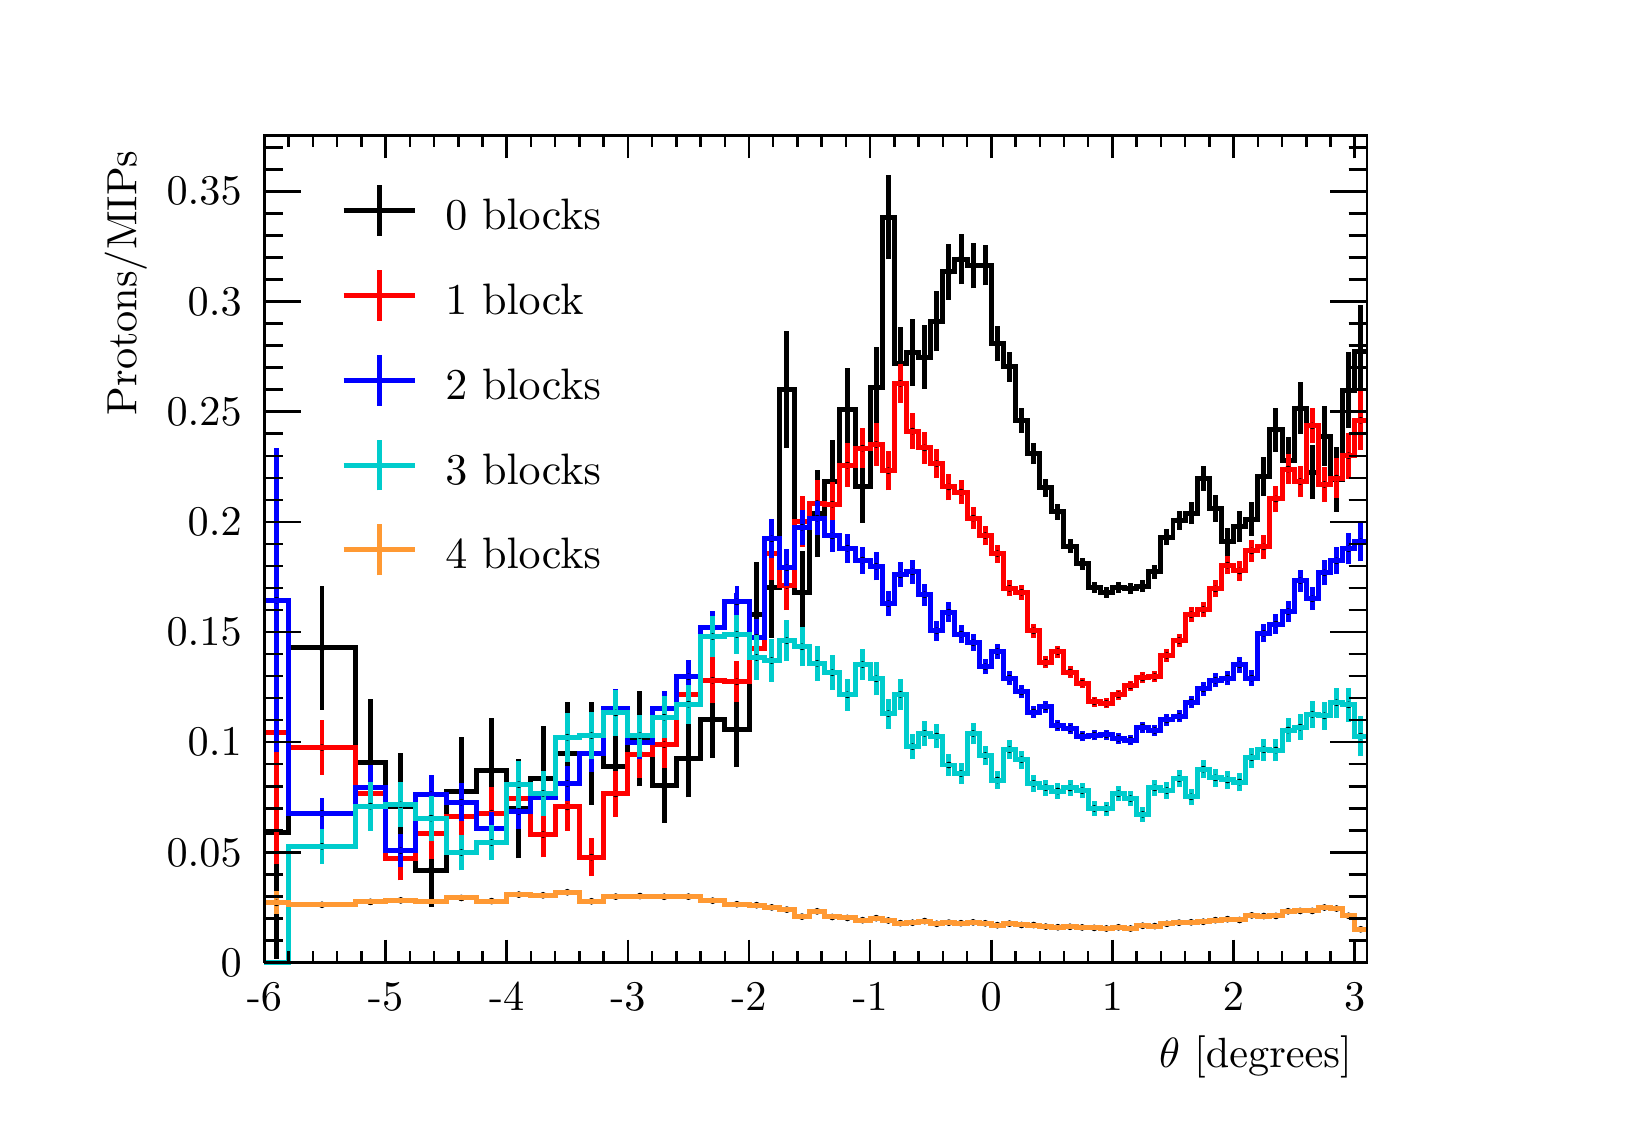
\begin{tikzpicture}
\pgfdeclareplotmark{cross} {
\pgfpathmoveto{\pgfpoint{-0.3\pgfplotmarksize}{\pgfplotmarksize}}
\pgfpathlineto{\pgfpoint{+0.3\pgfplotmarksize}{\pgfplotmarksize}}
\pgfpathlineto{\pgfpoint{+0.3\pgfplotmarksize}{0.3\pgfplotmarksize}}
\pgfpathlineto{\pgfpoint{+1\pgfplotmarksize}{0.3\pgfplotmarksize}}
\pgfpathlineto{\pgfpoint{+1\pgfplotmarksize}{-0.3\pgfplotmarksize}}
\pgfpathlineto{\pgfpoint{+0.3\pgfplotmarksize}{-0.3\pgfplotmarksize}}
\pgfpathlineto{\pgfpoint{+0.3\pgfplotmarksize}{-1.\pgfplotmarksize}}
\pgfpathlineto{\pgfpoint{-0.3\pgfplotmarksize}{-1.\pgfplotmarksize}}
\pgfpathlineto{\pgfpoint{-0.3\pgfplotmarksize}{-0.3\pgfplotmarksize}}
\pgfpathlineto{\pgfpoint{-1.\pgfplotmarksize}{-0.3\pgfplotmarksize}}
\pgfpathlineto{\pgfpoint{-1.\pgfplotmarksize}{0.3\pgfplotmarksize}}
\pgfpathlineto{\pgfpoint{-0.3\pgfplotmarksize}{0.3\pgfplotmarksize}}
\pgfpathclose
\pgfusepathqstroke
}
\pgfdeclareplotmark{cross*} {
\pgfpathmoveto{\pgfpoint{-0.3\pgfplotmarksize}{\pgfplotmarksize}}
\pgfpathlineto{\pgfpoint{+0.3\pgfplotmarksize}{\pgfplotmarksize}}
\pgfpathlineto{\pgfpoint{+0.3\pgfplotmarksize}{0.3\pgfplotmarksize}}
\pgfpathlineto{\pgfpoint{+1\pgfplotmarksize}{0.3\pgfplotmarksize}}
\pgfpathlineto{\pgfpoint{+1\pgfplotmarksize}{-0.3\pgfplotmarksize}}
\pgfpathlineto{\pgfpoint{+0.3\pgfplotmarksize}{-0.3\pgfplotmarksize}}
\pgfpathlineto{\pgfpoint{+0.3\pgfplotmarksize}{-1.\pgfplotmarksize}}
\pgfpathlineto{\pgfpoint{-0.3\pgfplotmarksize}{-1.\pgfplotmarksize}}
\pgfpathlineto{\pgfpoint{-0.3\pgfplotmarksize}{-0.3\pgfplotmarksize}}
\pgfpathlineto{\pgfpoint{-1.\pgfplotmarksize}{-0.3\pgfplotmarksize}}
\pgfpathlineto{\pgfpoint{-1.\pgfplotmarksize}{0.3\pgfplotmarksize}}
\pgfpathlineto{\pgfpoint{-0.3\pgfplotmarksize}{0.3\pgfplotmarksize}}
\pgfpathclose
\pgfusepathqfillstroke
}
\pgfdeclareplotmark{newstar} {
\pgfpathmoveto{\pgfqpoint{0pt}{\pgfplotmarksize}}
\pgfpathlineto{\pgfqpointpolar{44}{0.5\pgfplotmarksize}}
\pgfpathlineto{\pgfqpointpolar{18}{\pgfplotmarksize}}
\pgfpathlineto{\pgfqpointpolar{-20}{0.5\pgfplotmarksize}}
\pgfpathlineto{\pgfqpointpolar{-54}{\pgfplotmarksize}}
\pgfpathlineto{\pgfqpointpolar{-90}{0.5\pgfplotmarksize}}
\pgfpathlineto{\pgfqpointpolar{234}{\pgfplotmarksize}}
\pgfpathlineto{\pgfqpointpolar{198}{0.5\pgfplotmarksize}}
\pgfpathlineto{\pgfqpointpolar{162}{\pgfplotmarksize}}
\pgfpathlineto{\pgfqpointpolar{134}{0.5\pgfplotmarksize}}
\pgfpathclose
\pgfusepathqstroke
}
\pgfdeclareplotmark{newstar*} {
\pgfpathmoveto{\pgfqpoint{0pt}{\pgfplotmarksize}}
\pgfpathlineto{\pgfqpointpolar{44}{0.5\pgfplotmarksize}}
\pgfpathlineto{\pgfqpointpolar{18}{\pgfplotmarksize}}
\pgfpathlineto{\pgfqpointpolar{-20}{0.5\pgfplotmarksize}}
\pgfpathlineto{\pgfqpointpolar{-54}{\pgfplotmarksize}}
\pgfpathlineto{\pgfqpointpolar{-90}{0.5\pgfplotmarksize}}
\pgfpathlineto{\pgfqpointpolar{234}{\pgfplotmarksize}}
\pgfpathlineto{\pgfqpointpolar{198}{0.5\pgfplotmarksize}}
\pgfpathlineto{\pgfqpointpolar{162}{\pgfplotmarksize}}
\pgfpathlineto{\pgfqpointpolar{134}{0.5\pgfplotmarksize}}
\pgfpathclose
\pgfusepathqfillstroke
}
\definecolor{c}{rgb}{1,1,1};
\draw [color=c, fill=c] (0,0) rectangle (20,13.639);
\draw [color=c, fill=c] (3,1.77307) rectangle (17,12.2751);
\definecolor{c}{rgb}{0,0,0};
\draw [c,line width=0.9] (3,1.77307) -- (3,12.2751) -- (17,12.2751) -- (17,1.77307) -- (3,1.77307);
\definecolor{c}{rgb}{1,1,1};
\draw [color=c, fill=c] (3,1.77307) rectangle (17,12.2751);
\definecolor{c}{rgb}{0,0,0};
\draw [c,line width=0.9] (3,1.77307) -- (3,12.2751) -- (17,12.2751) -- (17,1.77307) -- (3,1.77307);
\draw [c,line width=0.9] (3,1.77307) -- (3.30769,1.77307) -- (3.30769,1.77307) -- (4.15385,1.77307) -- (4.15385,1.77307) -- (4.53846,1.77307) -- (4.53846,1.77307) -- (4.92308,1.77307) -- (4.92308,1.77307) -- (5.30769,1.77307) -- (5.30769,1.77307) --
 (5.69231,1.77307) -- (5.69231,1.77307) -- (6.07692,1.77307) -- (6.07692,1.77307) -- (6.38462,1.77307) -- (6.38462,1.77307) -- (6.69231,1.77307) -- (6.69231,1.77307) -- (7,1.77307) -- (7,1.77307) -- (7.30769,1.77307) -- (7.30769,1.77307) --
 (7.61538,1.77307) -- (7.61538,1.77307) -- (7.92308,1.77307) -- (7.92308,1.77307) -- (8.23077,1.77307) -- (8.23077,1.77307) -- (8.53846,1.77307) -- (8.53846,1.77307) -- (8.84615,1.77307) -- (8.84615,1.77307) -- (9.15385,1.77307) -- (9.15385,1.77307)
 -- (9.34615,1.77307) -- (9.34615,1.77307) -- (9.53846,1.77307) -- (9.53846,1.77307) -- (9.73077,1.77307) -- (9.73077,1.77307) -- (9.92308,1.77307) -- (9.92308,1.77307) -- (10.1154,1.77307) -- (10.1154,1.77307) -- (10.3077,1.77307) --
 (10.3077,1.77307) -- (10.5,1.77307) -- (10.5,1.77307) -- (10.6923,1.77307) -- (10.6923,1.77307) -- (10.8462,1.77307) -- (10.8462,1.77307) -- (11,1.77307) -- (11,1.77307) -- (11.1538,1.77307) -- (11.1538,1.77307) -- (11.3077,1.77307) --
 (11.3077,1.77307) -- (11.4615,1.77307) -- (11.4615,1.77307) -- (11.6154,1.77307) -- (11.6154,1.77307) -- (11.7692,1.77307) -- (11.7692,1.77307) -- (11.9231,1.77307) -- (11.9231,1.77307) -- (12.0769,1.77307) -- (12.0769,1.77307) -- (12.2308,1.77307)
 -- (12.2308,1.77307) -- (12.3846,1.77307) -- (12.3846,1.77307) -- (12.5385,1.77307) -- (12.5385,1.77307) -- (12.6923,1.77307) -- (12.6923,1.77307) -- (12.8462,1.77307) -- (12.8462,1.77307) -- (13,1.77307) -- (13,1.77307) -- (13.1538,1.77307) --
 (13.1538,1.77307) -- (13.3077,1.77307) -- (13.3077,1.77307) -- (13.4615,1.77307) -- (13.4615,1.77307) -- (13.6154,1.77307) -- (13.6154,1.77307) -- (13.7692,1.77307) -- (13.7692,1.77307) -- (13.9231,1.77307) -- (13.9231,1.77307) -- (14.0769,1.77307)
 -- (14.0769,1.77307) -- (14.2308,1.77307) -- (14.2308,1.77307) -- (14.3846,1.77307) -- (14.3846,1.77307) -- (14.5385,1.77307) -- (14.5385,1.77307) -- (14.6923,1.77307) -- (14.6923,1.77307) -- (14.8462,1.77307) -- (14.8462,1.77307) -- (15,1.77307) --
 (15,1.77307) -- (15.1538,1.77307) -- (15.1538,1.77307) -- (15.3077,1.77307) -- (15.3077,1.77307) -- (15.4615,1.77307) -- (15.4615,1.77307) -- (15.6154,1.77307) -- (15.6154,1.77307) -- (15.7692,1.77307) -- (15.7692,1.77307) -- (15.9231,1.77307) --
 (15.9231,1.77307) -- (16.0769,1.77307) -- (16.0769,1.77307) -- (16.2308,1.77307) -- (16.2308,1.77307) -- (16.3846,1.77307) -- (16.3846,1.77307) -- (16.5385,1.77307) -- (16.5385,1.77307) -- (16.6923,1.77307) -- (16.6923,1.77307) -- (16.8462,1.77307)
 -- (16.8462,1.77307) -- (17,1.77307);
\draw [c,line width=0.9] (3,1.77307) -- (17,1.77307);
\draw [c,line width=0.9] (3,2.05948) -- (3,1.77307);
\draw [c,line width=0.9] (3.30769,1.91628) -- (3.30769,1.77307);
\draw [c,line width=0.9] (3.61538,1.91628) -- (3.61538,1.77307);
\draw [c,line width=0.9] (3.92308,1.91628) -- (3.92308,1.77307);
\draw [c,line width=0.9] (4.23077,1.91628) -- (4.23077,1.77307);
\draw [c,line width=0.9] (4.53846,2.05948) -- (4.53846,1.77307);
\draw [c,line width=0.9] (4.84615,1.91628) -- (4.84615,1.77307);
\draw [c,line width=0.9] (5.15385,1.91628) -- (5.15385,1.77307);
\draw [c,line width=0.9] (5.46154,1.91628) -- (5.46154,1.77307);
\draw [c,line width=0.9] (5.76923,1.91628) -- (5.76923,1.77307);
\draw [c,line width=0.9] (6.07692,2.05948) -- (6.07692,1.77307);
\draw [c,line width=0.9] (6.38462,1.91628) -- (6.38462,1.77307);
\draw [c,line width=0.9] (6.69231,1.91628) -- (6.69231,1.77307);
\draw [c,line width=0.9] (7,1.91628) -- (7,1.77307);
\draw [c,line width=0.9] (7.30769,1.91628) -- (7.30769,1.77307);
\draw [c,line width=0.9] (7.61538,2.05948) -- (7.61538,1.77307);
\draw [c,line width=0.9] (7.92308,1.91628) -- (7.92308,1.77307);
\draw [c,line width=0.9] (8.23077,1.91628) -- (8.23077,1.77307);
\draw [c,line width=0.9] (8.53846,1.91628) -- (8.53846,1.77307);
\draw [c,line width=0.9] (8.84615,1.91628) -- (8.84615,1.77307);
\draw [c,line width=0.9] (9.15385,2.05948) -- (9.15385,1.77307);
\draw [c,line width=0.9] (9.46154,1.91628) -- (9.46154,1.77307);
\draw [c,line width=0.9] (9.76923,1.91628) -- (9.76923,1.77307);
\draw [c,line width=0.9] (10.0769,1.91628) -- (10.0769,1.77307);
\draw [c,line width=0.9] (10.3846,1.91628) -- (10.3846,1.77307);
\draw [c,line width=0.9] (10.6923,2.05948) -- (10.6923,1.77307);
\draw [c,line width=0.9] (11,1.91628) -- (11,1.77307);
\draw [c,line width=0.9] (11.3077,1.91628) -- (11.3077,1.77307);
\draw [c,line width=0.9] (11.6154,1.91628) -- (11.6154,1.77307);
\draw [c,line width=0.9] (11.9231,1.91628) -- (11.9231,1.77307);
\draw [c,line width=0.9] (12.2308,2.05948) -- (12.2308,1.77307);
\draw [c,line width=0.9] (12.5385,1.91628) -- (12.5385,1.77307);
\draw [c,line width=0.9] (12.8462,1.91628) -- (12.8462,1.77307);
\draw [c,line width=0.9] (13.1538,1.91628) -- (13.1538,1.77307);
\draw [c,line width=0.9] (13.4615,1.91628) -- (13.4615,1.77307);
\draw [c,line width=0.9] (13.7692,2.05948) -- (13.7692,1.77307);
\draw [c,line width=0.9] (14.0769,1.91628) -- (14.0769,1.77307);
\draw [c,line width=0.9] (14.3846,1.91628) -- (14.3846,1.77307);
\draw [c,line width=0.9] (14.6923,1.91628) -- (14.6923,1.77307);
\draw [c,line width=0.9] (15,1.91628) -- (15,1.77307);
\draw [c,line width=0.9] (15.3077,2.05948) -- (15.3077,1.77307);
\draw [c,line width=0.9] (15.6154,1.91628) -- (15.6154,1.77307);
\draw [c,line width=0.9] (15.9231,1.91628) -- (15.9231,1.77307);
\draw [c,line width=0.9] (16.2308,1.91628) -- (16.2308,1.77307);
\draw [c,line width=0.9] (16.5385,1.91628) -- (16.5385,1.77307);
\draw [c,line width=0.9] (16.8462,2.05948) -- (16.8462,1.77307);
\draw [c,line width=0.9] (16.8462,2.05948) -- (16.8462,1.77307);
\draw [anchor=base] (3,1.15931) node[scale=1.52731, color=c, rotate=0]{-6};
\draw [anchor=base] (4.53846,1.15931) node[scale=1.52731, color=c, rotate=0]{-5};
\draw [anchor=base] (6.07692,1.15931) node[scale=1.52731, color=c, rotate=0]{-4};
\draw [anchor=base] (7.61538,1.15931) node[scale=1.52731, color=c, rotate=0]{-3};
\draw [anchor=base] (9.15385,1.15931) node[scale=1.52731, color=c, rotate=0]{-2};
\draw [anchor=base] (10.6923,1.15931) node[scale=1.52731, color=c, rotate=0]{-1};
\draw [anchor=base] (12.2308,1.15931) node[scale=1.52731, color=c, rotate=0]{0};
\draw [anchor=base] (13.7692,1.15931) node[scale=1.52731, color=c, rotate=0]{1};
\draw [anchor=base] (15.3077,1.15931) node[scale=1.52731, color=c, rotate=0]{2};
\draw [anchor=base] (16.8462,1.15931) node[scale=1.52731, color=c, rotate=0]{3};
\draw [anchor= east] (17,0.572837) node[scale=1.52731, color=c, rotate=0]{$\theta$ [degrees]};
\draw [c,line width=0.9] (3,12.2751) -- (17,12.2751);
\draw [c,line width=0.9] (3,11.9887) -- (3,12.2751);
\draw [c,line width=0.9] (3.30769,12.1319) -- (3.30769,12.2751);
\draw [c,line width=0.9] (3.61538,12.1319) -- (3.61538,12.2751);
\draw [c,line width=0.9] (3.92308,12.1319) -- (3.92308,12.2751);
\draw [c,line width=0.9] (4.23077,12.1319) -- (4.23077,12.2751);
\draw [c,line width=0.9] (4.53846,11.9887) -- (4.53846,12.2751);
\draw [c,line width=0.9] (4.84615,12.1319) -- (4.84615,12.2751);
\draw [c,line width=0.9] (5.15385,12.1319) -- (5.15385,12.2751);
\draw [c,line width=0.9] (5.46154,12.1319) -- (5.46154,12.2751);
\draw [c,line width=0.9] (5.76923,12.1319) -- (5.76923,12.2751);
\draw [c,line width=0.9] (6.07692,11.9887) -- (6.07692,12.2751);
\draw [c,line width=0.9] (6.38462,12.1319) -- (6.38462,12.2751);
\draw [c,line width=0.9] (6.69231,12.1319) -- (6.69231,12.2751);
\draw [c,line width=0.9] (7,12.1319) -- (7,12.2751);
\draw [c,line width=0.9] (7.30769,12.1319) -- (7.30769,12.2751);
\draw [c,line width=0.9] (7.61538,11.9887) -- (7.61538,12.2751);
\draw [c,line width=0.9] (7.92308,12.1319) -- (7.92308,12.2751);
\draw [c,line width=0.9] (8.23077,12.1319) -- (8.23077,12.2751);
\draw [c,line width=0.9] (8.53846,12.1319) -- (8.53846,12.2751);
\draw [c,line width=0.9] (8.84615,12.1319) -- (8.84615,12.2751);
\draw [c,line width=0.9] (9.15385,11.9887) -- (9.15385,12.2751);
\draw [c,line width=0.9] (9.46154,12.1319) -- (9.46154,12.2751);
\draw [c,line width=0.9] (9.76923,12.1319) -- (9.76923,12.2751);
\draw [c,line width=0.9] (10.0769,12.1319) -- (10.0769,12.2751);
\draw [c,line width=0.9] (10.3846,12.1319) -- (10.3846,12.2751);
\draw [c,line width=0.9] (10.6923,11.9887) -- (10.6923,12.2751);
\draw [c,line width=0.9] (11,12.1319) -- (11,12.2751);
\draw [c,line width=0.9] (11.3077,12.1319) -- (11.3077,12.2751);
\draw [c,line width=0.9] (11.6154,12.1319) -- (11.6154,12.2751);
\draw [c,line width=0.9] (11.9231,12.1319) -- (11.9231,12.2751);
\draw [c,line width=0.9] (12.2308,11.9887) -- (12.2308,12.2751);
\draw [c,line width=0.9] (12.5385,12.1319) -- (12.5385,12.2751);
\draw [c,line width=0.9] (12.8462,12.1319) -- (12.8462,12.2751);
\draw [c,line width=0.9] (13.1538,12.1319) -- (13.1538,12.2751);
\draw [c,line width=0.9] (13.4615,12.1319) -- (13.4615,12.2751);
\draw [c,line width=0.9] (13.7692,11.9887) -- (13.7692,12.2751);
\draw [c,line width=0.9] (14.0769,12.1319) -- (14.0769,12.2751);
\draw [c,line width=0.9] (14.3846,12.1319) -- (14.3846,12.2751);
\draw [c,line width=0.9] (14.6923,12.1319) -- (14.6923,12.2751);
\draw [c,line width=0.9] (15,12.1319) -- (15,12.2751);
\draw [c,line width=0.9] (15.3077,11.9887) -- (15.3077,12.2751);
\draw [c,line width=0.9] (15.6154,12.1319) -- (15.6154,12.2751);
\draw [c,line width=0.9] (15.9231,12.1319) -- (15.9231,12.2751);
\draw [c,line width=0.9] (16.2308,12.1319) -- (16.2308,12.2751);
\draw [c,line width=0.9] (16.5385,12.1319) -- (16.5385,12.2751);
\draw [c,line width=0.9] (16.8462,11.9887) -- (16.8462,12.2751);
\draw [c,line width=0.9] (16.8462,11.9887) -- (16.8462,12.2751);
\draw [c,line width=0.9] (3,1.77307) -- (3,12.2751);
\draw [c,line width=0.9] (3.462,1.77307) -- (3,1.77307);
\draw [c,line width=0.9] (3.231,2.05289) -- (3,2.05289);
\draw [c,line width=0.9] (3.231,2.33272) -- (3,2.33272);
\draw [c,line width=0.9] (3.231,2.61255) -- (3,2.61255);
\draw [c,line width=0.9] (3.231,2.89237) -- (3,2.89237);
\draw [c,line width=0.9] (3.462,3.1722) -- (3,3.1722);
\draw [c,line width=0.9] (3.231,3.45203) -- (3,3.45203);
\draw [c,line width=0.9] (3.231,3.73185) -- (3,3.73185);
\draw [c,line width=0.9] (3.231,4.01168) -- (3,4.01168);
\draw [c,line width=0.9] (3.231,4.29151) -- (3,4.29151);
\draw [c,line width=0.9] (3.462,4.57133) -- (3,4.57133);
\draw [c,line width=0.9] (3.231,4.85116) -- (3,4.85116);
\draw [c,line width=0.9] (3.231,5.13099) -- (3,5.13099);
\draw [c,line width=0.9] (3.231,5.41081) -- (3,5.41081);
\draw [c,line width=0.9] (3.231,5.69064) -- (3,5.69064);
\draw [c,line width=0.9] (3.462,5.97047) -- (3,5.97047);
\draw [c,line width=0.9] (3.231,6.25029) -- (3,6.25029);
\draw [c,line width=0.9] (3.231,6.53012) -- (3,6.53012);
\draw [c,line width=0.9] (3.231,6.80995) -- (3,6.80995);
\draw [c,line width=0.9] (3.231,7.08977) -- (3,7.08977);
\draw [c,line width=0.9] (3.462,7.3696) -- (3,7.3696);
\draw [c,line width=0.9] (3.231,7.64943) -- (3,7.64943);
\draw [c,line width=0.9] (3.231,7.92925) -- (3,7.92925);
\draw [c,line width=0.9] (3.231,8.20908) -- (3,8.20908);
\draw [c,line width=0.9] (3.231,8.48891) -- (3,8.48891);
\draw [c,line width=0.9] (3.462,8.76873) -- (3,8.76873);
\draw [c,line width=0.9] (3.231,9.04856) -- (3,9.04856);
\draw [c,line width=0.9] (3.231,9.32839) -- (3,9.32839);
\draw [c,line width=0.9] (3.231,9.60821) -- (3,9.60821);
\draw [c,line width=0.9] (3.231,9.88804) -- (3,9.88804);
\draw [c,line width=0.9] (3.462,10.1679) -- (3,10.1679);
\draw [c,line width=0.9] (3.231,10.4477) -- (3,10.4477);
\draw [c,line width=0.9] (3.231,10.7275) -- (3,10.7275);
\draw [c,line width=0.9] (3.231,11.0073) -- (3,11.0073);
\draw [c,line width=0.9] (3.231,11.2872) -- (3,11.2872);
\draw [c,line width=0.9] (3.462,11.567) -- (3,11.567);
\draw [c,line width=0.9] (3.462,11.567) -- (3,11.567);
\draw [c,line width=0.9] (3.231,11.8468) -- (3,11.8468);
\draw [c,line width=0.9] (3.231,12.1267) -- (3,12.1267);
\draw [anchor= east] (2.9,1.77307) node[scale=1.52731, color=c, rotate=0]{0};
\draw [anchor= east] (2.9,3.1722) node[scale=1.52731, color=c, rotate=0]{0.05};
\draw [anchor= east] (2.9,4.57133) node[scale=1.52731, color=c, rotate=0]{0.1};
\draw [anchor= east] (2.9,5.97047) node[scale=1.52731, color=c, rotate=0]{0.15};
\draw [anchor= east] (2.9,7.3696) node[scale=1.52731, color=c, rotate=0]{0.2};
\draw [anchor= east] (2.9,8.76873) node[scale=1.52731, color=c, rotate=0]{0.25};
\draw [anchor= east] (2.9,10.1679) node[scale=1.52731, color=c, rotate=0]{0.3};
\draw [anchor= east] (2.9,11.567) node[scale=1.52731, color=c, rotate=0]{0.35};
\draw [anchor= east] (1.24,12.2751) node[scale=1.52731, color=c, rotate=90]{  Protons/MIPs};
\draw [c,line width=0.9] (17,1.77307) -- (17,12.2751);
\draw [c,line width=0.9] (16.538,1.77307) -- (17,1.77307);
\draw [c,line width=0.9] (16.769,2.05289) -- (17,2.05289);
\draw [c,line width=0.9] (16.769,2.33272) -- (17,2.33272);
\draw [c,line width=0.9] (16.769,2.61255) -- (17,2.61255);
\draw [c,line width=0.9] (16.769,2.89237) -- (17,2.89237);
\draw [c,line width=0.9] (16.538,3.1722) -- (17,3.1722);
\draw [c,line width=0.9] (16.769,3.45203) -- (17,3.45203);
\draw [c,line width=0.9] (16.769,3.73185) -- (17,3.73185);
\draw [c,line width=0.9] (16.769,4.01168) -- (17,4.01168);
\draw [c,line width=0.9] (16.769,4.29151) -- (17,4.29151);
\draw [c,line width=0.9] (16.538,4.57133) -- (17,4.57133);
\draw [c,line width=0.9] (16.769,4.85116) -- (17,4.85116);
\draw [c,line width=0.9] (16.769,5.13099) -- (17,5.13099);
\draw [c,line width=0.9] (16.769,5.41081) -- (17,5.41081);
\draw [c,line width=0.9] (16.769,5.69064) -- (17,5.69064);
\draw [c,line width=0.9] (16.538,5.97047) -- (17,5.97047);
\draw [c,line width=0.9] (16.769,6.25029) -- (17,6.25029);
\draw [c,line width=0.9] (16.769,6.53012) -- (17,6.53012);
\draw [c,line width=0.9] (16.769,6.80995) -- (17,6.80995);
\draw [c,line width=0.9] (16.769,7.08977) -- (17,7.08977);
\draw [c,line width=0.9] (16.538,7.3696) -- (17,7.3696);
\draw [c,line width=0.9] (16.769,7.64943) -- (17,7.64943);
\draw [c,line width=0.9] (16.769,7.92925) -- (17,7.92925);
\draw [c,line width=0.9] (16.769,8.20908) -- (17,8.20908);
\draw [c,line width=0.9] (16.769,8.48891) -- (17,8.48891);
\draw [c,line width=0.9] (16.538,8.76873) -- (17,8.76873);
\draw [c,line width=0.9] (16.769,9.04856) -- (17,9.04856);
\draw [c,line width=0.9] (16.769,9.32839) -- (17,9.32839);
\draw [c,line width=0.9] (16.769,9.60821) -- (17,9.60821);
\draw [c,line width=0.9] (16.769,9.88804) -- (17,9.88804);
\draw [c,line width=0.9] (16.538,10.1679) -- (17,10.1679);
\draw [c,line width=0.9] (16.769,10.4477) -- (17,10.4477);
\draw [c,line width=0.9] (16.769,10.7275) -- (17,10.7275);
\draw [c,line width=0.9] (16.769,11.0073) -- (17,11.0073);
\draw [c,line width=0.9] (16.769,11.2872) -- (17,11.2872);
\draw [c,line width=0.9] (16.538,11.567) -- (17,11.567);
\draw [c,line width=0.9] (16.538,11.567) -- (17,11.567);
\draw [c,line width=0.9] (16.769,11.8468) -- (17,11.8468);
\draw [c,line width=0.9] (16.769,12.1267) -- (17,12.1267);
\draw [c,line width=1.8] (3.15385,1.82211) -- (3.15385,3.41911);
\draw [c,line width=1.8] (3.15385,3.41911) -- (3.15385,5.0161);
\foreach \P in {(3.15385,3.41911)}{\draw[mark options={color=c,fill=c},mark size=2.402402pt,mark=*,mark size=1pt] plot coordinates {\P};}
\draw [c,line width=1.8] (3.73077,4.98149) -- (3.73077,5.77059);
\draw [c,line width=1.8] (3.73077,5.77059) -- (3.73077,6.55969);
\foreach \P in {(3.73077,5.77059)}{\draw[mark options={color=c,fill=c},mark size=2.402402pt,mark=*,mark size=1pt] plot coordinates {\P};}
\draw [c,line width=1.8] (4.34615,3.5084) -- (4.34615,4.31694);
\draw [c,line width=1.8] (4.34615,4.31694) -- (4.34615,5.12549);
\foreach \P in {(4.34615,4.31694)}{\draw[mark options={color=c,fill=c},mark size=2.402402pt,mark=*,mark size=1pt] plot coordinates {\P};}
\draw [c,line width=1.8] (4.73077,3.07893) -- (4.73077,3.75414);
\draw [c,line width=1.8] (4.73077,3.75414) -- (4.73077,4.42935);
\foreach \P in {(4.73077,3.75414)}{\draw[mark options={color=c,fill=c},mark size=2.402402pt,mark=*,mark size=1pt] plot coordinates {\P};}
\draw [c,line width=1.8] (5.11538,2.47797) -- (5.11538,2.94716);
\draw [c,line width=1.8] (5.11538,2.94716) -- (5.11538,3.41635);
\foreach \P in {(5.11538,2.94716)}{\draw[mark options={color=c,fill=c},mark size=2.402402pt,mark=*,mark size=1pt] plot coordinates {\P};}
\draw [c,line width=1.8] (5.5,3.24904) -- (5.5,3.94413);
\draw [c,line width=1.8] (5.5,3.94413) -- (5.5,4.63923);
\foreach \P in {(5.5,3.94413)}{\draw[mark options={color=c,fill=c},mark size=2.402402pt,mark=*,mark size=1pt] plot coordinates {\P};}
\draw [c,line width=1.8] (5.88462,3.53511) -- (5.88462,4.20634);
\draw [c,line width=1.8] (5.88462,4.20634) -- (5.88462,4.87758);
\foreach \P in {(5.88462,4.20634)}{\draw[mark options={color=c,fill=c},mark size=2.402402pt,mark=*,mark size=1pt] plot coordinates {\P};}
\draw [c,line width=1.8] (6.23077,3.09766) -- (6.23077,3.72534);
\draw [c,line width=1.8] (6.23077,3.72534) -- (6.23077,4.35303);
\foreach \P in {(6.23077,3.72534)}{\draw[mark options={color=c,fill=c},mark size=2.402402pt,mark=*,mark size=1pt] plot coordinates {\P};}
\draw [c,line width=1.8] (6.53846,3.43175) -- (6.53846,4.10495);
\draw [c,line width=1.8] (6.53846,4.10495) -- (6.53846,4.77816);
\foreach \P in {(6.53846,4.10495)}{\draw[mark options={color=c,fill=c},mark size=2.402402pt,mark=*,mark size=1pt] plot coordinates {\P};}
\draw [c,line width=1.8] (6.84615,3.77705) -- (6.84615,4.42965);
\draw [c,line width=1.8] (6.84615,4.42965) -- (6.84615,5.08224);
\foreach \P in {(6.84615,4.42965)}{\draw[mark options={color=c,fill=c},mark size=2.402402pt,mark=*,mark size=1pt] plot coordinates {\P};}
\draw [c,line width=1.8] (7.15385,3.77705) -- (7.15385,4.42965);
\draw [c,line width=1.8] (7.15385,4.42965) -- (7.15385,5.08224);
\foreach \P in {(7.15385,4.42965)}{\draw[mark options={color=c,fill=c},mark size=2.402402pt,mark=*,mark size=1pt] plot coordinates {\P};}
\draw [c,line width=1.8] (7.46154,3.68708) -- (7.46154,4.26367);
\draw [c,line width=1.8] (7.46154,4.26367) -- (7.46154,4.84026);
\foreach \P in {(7.46154,4.26367)}{\draw[mark options={color=c,fill=c},mark size=2.402402pt,mark=*,mark size=1pt] plot coordinates {\P};}
\draw [c,line width=1.8] (7.76923,4.01178) -- (7.76923,4.61395);
\draw [c,line width=1.8] (7.76923,4.61395) -- (7.76923,5.21612);
\foreach \P in {(7.76923,4.61395)}{\draw[mark options={color=c,fill=c},mark size=2.402402pt,mark=*,mark size=1pt] plot coordinates {\P};}
\draw [c,line width=1.8] (8.07692,3.54651) -- (8.07692,4.01595);
\draw [c,line width=1.8] (8.07692,4.01595) -- (8.07692,4.48539);
\foreach \P in {(8.07692,4.01595)}{\draw[mark options={color=c,fill=c},mark size=2.402402pt,mark=*,mark size=1pt] plot coordinates {\P};}
\draw [c,line width=1.8] (8.38461,3.8704) -- (8.38461,4.36405);
\draw [c,line width=1.8] (8.38461,4.36405) -- (8.38461,4.85771);
\foreach \P in {(8.38461,4.36405)}{\draw[mark options={color=c,fill=c},mark size=2.402402pt,mark=*,mark size=1pt] plot coordinates {\P};}
\draw [c,line width=1.8] (8.69231,4.37658) -- (8.69231,4.85449);
\draw [c,line width=1.8] (8.69231,4.85449) -- (8.69231,5.3324);
\foreach \P in {(8.69231,4.85449)}{\draw[mark options={color=c,fill=c},mark size=2.402402pt,mark=*,mark size=1pt] plot coordinates {\P};}
\draw [c,line width=1.8] (9,4.2563) -- (9,4.73696);
\draw [c,line width=1.8] (9,4.73696) -- (9,5.21762);
\foreach \P in {(9,4.73696)}{\draw[mark options={color=c,fill=c},mark size=2.402402pt,mark=*,mark size=1pt] plot coordinates {\P};}
\draw [c,line width=1.8] (9.25,5.53021) -- (9.25,6.19768);
\draw [c,line width=1.8] (9.25,6.19768) -- (9.25,6.86514);
\foreach \P in {(9.25,6.19768)}{\draw[mark options={color=c,fill=c},mark size=2.402402pt,mark=*,mark size=1pt] plot coordinates {\P};}
\draw [c,line width=1.8] (9.44231,5.9002) -- (9.44231,6.54048);
\draw [c,line width=1.8] (9.44231,6.54048) -- (9.44231,7.18077);
\foreach \P in {(9.44231,6.54048)}{\draw[mark options={color=c,fill=c},mark size=2.402402pt,mark=*,mark size=1pt] plot coordinates {\P};}
\draw [c,line width=1.8] (9.63461,8.30763) -- (9.63461,9.05061);
\draw [c,line width=1.8] (9.63461,9.05061) -- (9.63461,9.79359);
\foreach \P in {(9.63461,9.05061)}{\draw[mark options={color=c,fill=c},mark size=2.402402pt,mark=*,mark size=1pt] plot coordinates {\P};}
\draw [c,line width=1.8] (9.82692,5.94121) -- (9.82692,6.473);
\draw [c,line width=1.8] (9.82692,6.473) -- (9.82692,7.00478);
\foreach \P in {(9.82692,6.473)}{\draw[mark options={color=c,fill=c},mark size=2.402402pt,mark=*,mark size=1pt] plot coordinates {\P};}
\draw [c,line width=1.8] (10.0192,6.92282) -- (10.0192,7.47827);
\draw [c,line width=1.8] (10.0192,7.47827) -- (10.0192,8.03372);
\foreach \P in {(10.0192,7.47827)}{\draw[mark options={color=c,fill=c},mark size=2.402402pt,mark=*,mark size=1pt] plot coordinates {\P};}
\draw [c,line width=1.8] (10.2115,7.34742) -- (10.2115,7.87945);
\draw [c,line width=1.8] (10.2115,7.87945) -- (10.2115,8.41148);
\foreach \P in {(10.2115,7.87945)}{\draw[mark options={color=c,fill=c},mark size=2.402402pt,mark=*,mark size=1pt] plot coordinates {\P};}
\draw [c,line width=1.8] (10.4038,8.26812) -- (10.4038,8.79513);
\draw [c,line width=1.8] (10.4038,8.79513) -- (10.4038,9.32215);
\foreach \P in {(10.4038,8.79513)}{\draw[mark options={color=c,fill=c},mark size=2.402402pt,mark=*,mark size=1pt] plot coordinates {\P};}
\draw [c,line width=1.8] (10.5962,7.35913) -- (10.5962,7.8128);
\draw [c,line width=1.8] (10.5962,7.8128) -- (10.5962,8.26647);
\foreach \P in {(10.5962,7.8128)}{\draw[mark options={color=c,fill=c},mark size=2.402402pt,mark=*,mark size=1pt] plot coordinates {\P};}
\draw [c,line width=1.8] (10.7692,8.57136) -- (10.7692,9.07912);
\draw [c,line width=1.8] (10.7692,9.07912) -- (10.7692,9.58688);
\foreach \P in {(10.7692,9.07912)}{\draw[mark options={color=c,fill=c},mark size=2.402402pt,mark=*,mark size=1pt] plot coordinates {\P};}
\draw [c,line width=1.8] (10.9231,10.702) -- (10.9231,11.2385);
\draw [c,line width=1.8] (10.9231,11.2385) -- (10.9231,11.775);
\foreach \P in {(10.9231,11.2385)}{\draw[mark options={color=c,fill=c},mark size=2.402402pt,mark=*,mark size=1pt] plot coordinates {\P};}
\draw [c,line width=1.8] (11.0769,8.92018) -- (11.0769,9.38038);
\draw [c,line width=1.8] (11.0769,9.38038) -- (11.0769,9.84057);
\foreach \P in {(11.0769,9.38038)}{\draw[mark options={color=c,fill=c},mark size=2.402402pt,mark=*,mark size=1pt] plot coordinates {\P};}
\draw [c,line width=1.8] (11.2308,9.09999) -- (11.2308,9.52459);
\draw [c,line width=1.8] (11.2308,9.52459) -- (11.2308,9.94918);
\foreach \P in {(11.2308,9.52459)}{\draw[mark options={color=c,fill=c},mark size=2.402402pt,mark=*,mark size=1pt] plot coordinates {\P};}
\draw [c,line width=1.8] (11.3846,9.06099) -- (11.3846,9.46252);
\draw [c,line width=1.8] (11.3846,9.46252) -- (11.3846,9.86404);
\foreach \P in {(11.3846,9.46252)}{\draw[mark options={color=c,fill=c},mark size=2.402402pt,mark=*,mark size=1pt] plot coordinates {\P};}
\draw [c,line width=1.8] (11.5385,9.53396) -- (11.5385,9.91671);
\draw [c,line width=1.8] (11.5385,9.91671) -- (11.5385,10.2995);
\foreach \P in {(11.5385,9.91671)}{\draw[mark options={color=c,fill=c},mark size=2.402402pt,mark=*,mark size=1pt] plot coordinates {\P};}
\draw [c,line width=1.8] (11.6923,10.1909) -- (11.6923,10.5434);
\draw [c,line width=1.8] (11.6923,10.5434) -- (11.6923,10.896);
\foreach \P in {(11.6923,10.5434)}{\draw[mark options={color=c,fill=c},mark size=2.402402pt,mark=*,mark size=1pt] plot coordinates {\P};}
\draw [c,line width=1.8] (11.8462,10.3843) -- (11.8462,10.707);
\draw [c,line width=1.8] (11.8462,10.707) -- (11.8462,11.0296);
\foreach \P in {(11.8462,10.707)}{\draw[mark options={color=c,fill=c},mark size=2.402402pt,mark=*,mark size=1pt] plot coordinates {\P};}
\draw [c,line width=1.8] (12,10.3355) -- (12,10.625);
\draw [c,line width=1.8] (12,10.625) -- (12,10.9146);
\foreach \P in {(12,10.625)}{\draw[mark options={color=c,fill=c},mark size=2.402402pt,mark=*,mark size=1pt] plot coordinates {\P};}
\draw [c,line width=1.8] (12.1538,10.3727) -- (12.1538,10.6278);
\draw [c,line width=1.8] (12.1538,10.6278) -- (12.1538,10.8828);
\foreach \P in {(12.1538,10.6278)}{\draw[mark options={color=c,fill=c},mark size=2.402402pt,mark=*,mark size=1pt] plot coordinates {\P};}
\draw [c,line width=1.8] (12.3077,9.40941) -- (12.3077,9.63297);
\draw [c,line width=1.8] (12.3077,9.63297) -- (12.3077,9.85653);
\foreach \P in {(12.3077,9.63297)}{\draw[mark options={color=c,fill=c},mark size=2.402402pt,mark=*,mark size=1pt] plot coordinates {\P};}
\draw [c,line width=1.8] (12.4615,9.14774) -- (12.4615,9.34012);
\draw [c,line width=1.8] (12.4615,9.34012) -- (12.4615,9.53249);
\foreach \P in {(12.4615,9.34012)}{\draw[mark options={color=c,fill=c},mark size=2.402402pt,mark=*,mark size=1pt] plot coordinates {\P};}
\draw [c,line width=1.8] (12.6154,8.50404) -- (12.6154,8.66245);
\draw [c,line width=1.8] (12.6154,8.66245) -- (12.6154,8.82085);
\foreach \P in {(12.6154,8.66245)}{\draw[mark options={color=c,fill=c},mark size=2.402402pt,mark=*,mark size=1pt] plot coordinates {\P};}
\draw [c,line width=1.8] (12.7692,8.10435) -- (12.7692,8.2387);
\draw [c,line width=1.8] (12.7692,8.2387) -- (12.7692,8.37306);
\foreach \P in {(12.7692,8.2387)}{\draw[mark options={color=c,fill=c},mark size=2.402402pt,mark=*,mark size=1pt] plot coordinates {\P};}
\draw [c,line width=1.8] (12.9231,7.68928) -- (12.9231,7.80332);
\draw [c,line width=1.8] (12.9231,7.80332) -- (12.9231,7.91735);
\foreach \P in {(12.9231,7.80332)}{\draw[mark options={color=c,fill=c},mark size=2.402402pt,mark=*,mark size=1pt] plot coordinates {\P};}
\draw [c,line width=1.8] (13.0769,7.39569) -- (13.0769,7.49512);
\draw [c,line width=1.8] (13.0769,7.49512) -- (13.0769,7.59454);
\foreach \P in {(13.0769,7.49512)}{\draw[mark options={color=c,fill=c},mark size=2.402402pt,mark=*,mark size=1pt] plot coordinates {\P};}
\draw [c,line width=1.8] (13.2308,6.97329) -- (13.2308,7.06043);
\draw [c,line width=1.8] (13.2308,7.06043) -- (13.2308,7.14758);
\foreach \P in {(13.2308,7.06043)}{\draw[mark options={color=c,fill=c},mark size=2.402402pt,mark=*,mark size=1pt] plot coordinates {\P};}
\draw [c,line width=1.8] (13.3846,6.7589) -- (13.3846,6.83628);
\draw [c,line width=1.8] (13.3846,6.83628) -- (13.3846,6.91366);
\foreach \P in {(13.3846,6.83628)}{\draw[mark options={color=c,fill=c},mark size=2.402402pt,mark=*,mark size=1pt] plot coordinates {\P};}
\draw [c,line width=1.8] (13.5385,6.46938) -- (13.5385,6.53954);
\draw [c,line width=1.8] (13.5385,6.53954) -- (13.5385,6.60971);
\foreach \P in {(13.5385,6.53954)}{\draw[mark options={color=c,fill=c},mark size=2.402402pt,mark=*,mark size=1pt] plot coordinates {\P};}
\draw [c,line width=1.8] (13.6923,6.40391) -- (13.6923,6.47146);
\draw [c,line width=1.8] (13.6923,6.47146) -- (13.6923,6.539);
\foreach \P in {(13.6923,6.47146)}{\draw[mark options={color=c,fill=c},mark size=2.402402pt,mark=*,mark size=1pt] plot coordinates {\P};}
\draw [c,line width=1.8] (13.8462,6.47055) -- (13.8462,6.53894);
\draw [c,line width=1.8] (13.8462,6.53894) -- (13.8462,6.60733);
\foreach \P in {(13.8462,6.53894)}{\draw[mark options={color=c,fill=c},mark size=2.402402pt,mark=*,mark size=1pt] plot coordinates {\P};}
\draw [c,line width=1.8] (14,6.45026) -- (14,6.52192);
\draw [c,line width=1.8] (14,6.52192) -- (14,6.59357);
\foreach \P in {(14,6.52192)}{\draw[mark options={color=c,fill=c},mark size=2.402402pt,mark=*,mark size=1pt] plot coordinates {\P};}
\draw [c,line width=1.8] (14.1538,6.47551) -- (14.1538,6.55327);
\draw [c,line width=1.8] (14.1538,6.55327) -- (14.1538,6.63103);
\foreach \P in {(14.1538,6.55327)}{\draw[mark options={color=c,fill=c},mark size=2.402402pt,mark=*,mark size=1pt] plot coordinates {\P};}
\draw [c,line width=1.8] (14.3077,6.64793) -- (14.3077,6.73649);
\draw [c,line width=1.8] (14.3077,6.73649) -- (14.3077,6.82506);
\foreach \P in {(14.3077,6.73649)}{\draw[mark options={color=c,fill=c},mark size=2.402402pt,mark=*,mark size=1pt] plot coordinates {\P};}
\draw [c,line width=1.8] (14.4615,7.07039) -- (14.4615,7.1755);
\draw [c,line width=1.8] (14.4615,7.1755) -- (14.4615,7.28061);
\foreach \P in {(14.4615,7.1755)}{\draw[mark options={color=c,fill=c},mark size=2.402402pt,mark=*,mark size=1pt] plot coordinates {\P};}
\draw [c,line width=1.8] (14.6154,7.27076) -- (14.6154,7.39177);
\draw [c,line width=1.8] (14.6154,7.39177) -- (14.6154,7.51279);
\foreach \P in {(14.6154,7.39177)}{\draw[mark options={color=c,fill=c},mark size=2.402402pt,mark=*,mark size=1pt] plot coordinates {\P};}
\draw [c,line width=1.8] (14.7692,7.34057) -- (14.7692,7.47851);
\draw [c,line width=1.8] (14.7692,7.47851) -- (14.7692,7.61646);
\foreach \P in {(14.7692,7.47851)}{\draw[mark options={color=c,fill=c},mark size=2.402402pt,mark=*,mark size=1pt] plot coordinates {\P};}
\draw [c,line width=1.8] (14.9231,7.76493) -- (14.9231,7.92186);
\draw [c,line width=1.8] (14.9231,7.92186) -- (14.9231,8.07879);
\foreach \P in {(14.9231,7.92186)}{\draw[mark options={color=c,fill=c},mark size=2.402402pt,mark=*,mark size=1pt] plot coordinates {\P};}
\draw [c,line width=1.8] (15.0769,7.36896) -- (15.0769,7.53787);
\draw [c,line width=1.8] (15.0769,7.53787) -- (15.0769,7.70678);
\foreach \P in {(15.0769,7.53787)}{\draw[mark options={color=c,fill=c},mark size=2.402402pt,mark=*,mark size=1pt] plot coordinates {\P};}
\draw [c,line width=1.8] (15.2308,6.94021) -- (15.2308,7.11766);
\draw [c,line width=1.8] (15.2308,7.11766) -- (15.2308,7.29511);
\foreach \P in {(15.2308,7.11766)}{\draw[mark options={color=c,fill=c},mark size=2.402402pt,mark=*,mark size=1pt] plot coordinates {\P};}
\draw [c,line width=1.8] (15.3846,7.11146) -- (15.3846,7.31065);
\draw [c,line width=1.8] (15.3846,7.31065) -- (15.3846,7.50984);
\foreach \P in {(15.3846,7.31065)}{\draw[mark options={color=c,fill=c},mark size=2.402402pt,mark=*,mark size=1pt] plot coordinates {\P};}
\draw [c,line width=1.8] (15.5385,7.18993) -- (15.5385,7.40435);
\draw [c,line width=1.8] (15.5385,7.40435) -- (15.5385,7.61877);
\foreach \P in {(15.5385,7.40435)}{\draw[mark options={color=c,fill=c},mark size=2.402402pt,mark=*,mark size=1pt] plot coordinates {\P};}
\draw [c,line width=1.8] (15.6923,7.69841) -- (15.6923,7.94405);
\draw [c,line width=1.8] (15.6923,7.94405) -- (15.6923,8.18969);
\foreach \P in {(15.6923,7.94405)}{\draw[mark options={color=c,fill=c},mark size=2.402402pt,mark=*,mark size=1pt] plot coordinates {\P};}
\draw [c,line width=1.8] (15.8462,8.2613) -- (15.8462,8.53778);
\draw [c,line width=1.8] (15.8462,8.53778) -- (15.8462,8.81425);
\foreach \P in {(15.8462,8.53778)}{\draw[mark options={color=c,fill=c},mark size=2.402402pt,mark=*,mark size=1pt] plot coordinates {\P};}
\draw [c,line width=1.8] (16,7.85164) -- (16,8.14729);
\draw [c,line width=1.8] (16,8.14729) -- (16,8.44294);
\foreach \P in {(16,8.14729)}{\draw[mark options={color=c,fill=c},mark size=2.402402pt,mark=*,mark size=1pt] plot coordinates {\P};}
\draw [c,line width=1.8] (16.1538,8.48633) -- (16.1538,8.81479);
\draw [c,line width=1.8] (16.1538,8.81479) -- (16.1538,9.14325);
\foreach \P in {(16.1538,8.81479)}{\draw[mark options={color=c,fill=c},mark size=2.402402pt,mark=*,mark size=1pt] plot coordinates {\P};}
\draw [c,line width=1.8] (16.3077,7.65829) -- (16.3077,7.99945);
\draw [c,line width=1.8] (16.3077,7.99945) -- (16.3077,8.34061);
\foreach \P in {(16.3077,7.99945)}{\draw[mark options={color=c,fill=c},mark size=2.402402pt,mark=*,mark size=1pt] plot coordinates {\P};}
\draw [c,line width=1.8] (16.4615,8.08155) -- (16.4615,8.45969);
\draw [c,line width=1.8] (16.4615,8.45969) -- (16.4615,8.83783);
\foreach \P in {(16.4615,8.45969)}{\draw[mark options={color=c,fill=c},mark size=2.402402pt,mark=*,mark size=1pt] plot coordinates {\P};}
\draw [c,line width=1.8] (16.6154,7.49771) -- (16.6154,7.90625);
\draw [c,line width=1.8] (16.6154,7.90625) -- (16.6154,8.31479);
\foreach \P in {(16.6154,7.90625)}{\draw[mark options={color=c,fill=c},mark size=2.402402pt,mark=*,mark size=1pt] plot coordinates {\P};}
\draw [c,line width=1.8] (16.7692,8.55682) -- (16.7692,9.04073);
\draw [c,line width=1.8] (16.7692,9.04073) -- (16.7692,9.52463);
\foreach \P in {(16.7692,9.04073)}{\draw[mark options={color=c,fill=c},mark size=2.402402pt,mark=*,mark size=1pt] plot coordinates {\P};}
\draw [c,line width=1.8] (16.9231,8.93468) -- (16.9231,9.5319);
\draw [c,line width=1.8] (16.9231,9.5319) -- (16.9231,10.1291);
\foreach \P in {(16.9231,9.5319)}{\draw[mark options={color=c,fill=c},mark size=2.402402pt,mark=*,mark size=1pt] plot coordinates {\P};}
\draw [c,line width=1.8] (3,3.41911) -- (3.30769,3.41911) -- (3.30769,5.77059) -- (4.15385,5.77059) -- (4.15385,4.31694) -- (4.53846,4.31694) -- (4.53846,3.75414) -- (4.92308,3.75414) -- (4.92308,2.94716) -- (5.30769,2.94716) -- (5.30769,3.94413) --
 (5.69231,3.94413) -- (5.69231,4.20634) -- (6.07692,4.20634) -- (6.07692,3.72534) -- (6.38462,3.72534) -- (6.38462,4.10495) -- (6.69231,4.10495) -- (6.69231,4.42965) -- (7,4.42965) -- (7,4.42965) -- (7.30769,4.42965) -- (7.30769,4.26367) --
 (7.61538,4.26367) -- (7.61538,4.61395) -- (7.92308,4.61395) -- (7.92308,4.01595) -- (8.23077,4.01595) -- (8.23077,4.36405) -- (8.53846,4.36405) -- (8.53846,4.85449) -- (8.84615,4.85449) -- (8.84615,4.73696) -- (9.15385,4.73696) -- (9.15385,6.19768)
 -- (9.34615,6.19768) -- (9.34615,6.54048) -- (9.53846,6.54048) -- (9.53846,9.05061) -- (9.73077,9.05061) -- (9.73077,6.473) -- (9.92308,6.473) -- (9.92308,7.47827) -- (10.1154,7.47827) -- (10.1154,7.87945) -- (10.3077,7.87945) -- (10.3077,8.79513)
 -- (10.5,8.79513) -- (10.5,7.8128) -- (10.6923,7.8128) -- (10.6923,9.07912) -- (10.8462,9.07912) -- (10.8462,11.2385) -- (11,11.2385) -- (11,9.38038) -- (11.1538,9.38038) -- (11.1538,9.52459) -- (11.3077,9.52459) -- (11.3077,9.46252) --
 (11.4615,9.46252) -- (11.4615,9.91671) -- (11.6154,9.91671) -- (11.6154,10.5434) -- (11.7692,10.5434) -- (11.7692,10.707) -- (11.9231,10.707) -- (11.9231,10.625) -- (12.0769,10.625) -- (12.0769,10.6278) -- (12.2308,10.6278) -- (12.2308,9.63297) --
 (12.3846,9.63297) -- (12.3846,9.34012) -- (12.5385,9.34012) -- (12.5385,8.66245) -- (12.6923,8.66245) -- (12.6923,8.2387) -- (12.8462,8.2387) -- (12.8462,7.80332) -- (13,7.80332) -- (13,7.49512) -- (13.1538,7.49512) -- (13.1538,7.06043) --
 (13.3077,7.06043) -- (13.3077,6.83628) -- (13.4615,6.83628) -- (13.4615,6.53954) -- (13.6154,6.53954) -- (13.6154,6.47146) -- (13.7692,6.47146) -- (13.7692,6.53894) -- (13.9231,6.53894) -- (13.9231,6.52192) -- (14.0769,6.52192) -- (14.0769,6.55327)
 -- (14.2308,6.55327) -- (14.2308,6.73649) -- (14.3846,6.73649) -- (14.3846,7.1755) -- (14.5385,7.1755) -- (14.5385,7.39177) -- (14.6923,7.39177) -- (14.6923,7.47851) -- (14.8462,7.47851) -- (14.8462,7.92186) -- (15,7.92186) -- (15,7.53787) --
 (15.1538,7.53787) -- (15.1538,7.11766) -- (15.3077,7.11766) -- (15.3077,7.31065) -- (15.4615,7.31065) -- (15.4615,7.40435) -- (15.6154,7.40435) -- (15.6154,7.94405) -- (15.7692,7.94405) -- (15.7692,8.53778) -- (15.9231,8.53778) -- (15.9231,8.14729)
 -- (16.0769,8.14729) -- (16.0769,8.81479) -- (16.2308,8.81479) -- (16.2308,7.99945) -- (16.3846,7.99945) -- (16.3846,8.45969) -- (16.5385,8.45969) -- (16.5385,7.90625) -- (16.6923,7.90625) -- (16.6923,9.04073) -- (16.8462,9.04073) --
 (16.8462,9.5319) -- (17,9.5319);
\definecolor{c}{rgb}{1,0,0};
\draw [c,line width=1.8] (3.15385,3.01897) -- (3.15385,4.69533);
\draw [c,line width=1.8] (3.15385,4.69533) -- (3.15385,6.3717);
\definecolor{c}{rgb}{0,0,0};
\foreach \P in {(3.15385,4.69533)}{\draw[mark options={color=c,fill=c},mark size=2.402402pt,mark=*,mark size=1pt] plot coordinates {\P};}
\definecolor{c}{rgb}{1,0,0};
\draw [c,line width=1.8] (3.73077,4.15602) -- (3.73077,4.5033);
\draw [c,line width=1.8] (3.73077,4.5033) -- (3.73077,4.85059);
\definecolor{c}{rgb}{0,0,0};
\foreach \P in {(3.73077,4.5033)}{\draw[mark options={color=c,fill=c},mark size=2.402402pt,mark=*,mark size=1pt] plot coordinates {\P};}
\definecolor{c}{rgb}{1,0,0};
\draw [c,line width=1.8] (4.34615,3.5692) -- (4.34615,3.92217);
\draw [c,line width=1.8] (4.34615,3.92217) -- (4.34615,4.27514);
\definecolor{c}{rgb}{0,0,0};
\foreach \P in {(4.34615,3.92217)}{\draw[mark options={color=c,fill=c},mark size=2.402402pt,mark=*,mark size=1pt] plot coordinates {\P};}
\definecolor{c}{rgb}{1,0,0};
\draw [c,line width=1.8] (4.73077,2.8168) -- (4.73077,3.09583);
\draw [c,line width=1.8] (4.73077,3.09583) -- (4.73077,3.37486);
\definecolor{c}{rgb}{0,0,0};
\foreach \P in {(4.73077,3.09583)}{\draw[mark options={color=c,fill=c},mark size=2.402402pt,mark=*,mark size=1pt] plot coordinates {\P};}
\definecolor{c}{rgb}{1,0,0};
\draw [c,line width=1.8] (5.11538,3.08425) -- (5.11538,3.40645);
\draw [c,line width=1.8] (5.11538,3.40645) -- (5.11538,3.72865);
\definecolor{c}{rgb}{0,0,0};
\foreach \P in {(5.11538,3.40645)}{\draw[mark options={color=c,fill=c},mark size=2.402402pt,mark=*,mark size=1pt] plot coordinates {\P};}
\definecolor{c}{rgb}{1,0,0};
\draw [c,line width=1.8] (5.5,3.3103) -- (5.5,3.63009);
\draw [c,line width=1.8] (5.5,3.63009) -- (5.5,3.94989);
\definecolor{c}{rgb}{0,0,0};
\foreach \P in {(5.5,3.63009)}{\draw[mark options={color=c,fill=c},mark size=2.402402pt,mark=*,mark size=1pt] plot coordinates {\P};}
\definecolor{c}{rgb}{1,0,0};
\draw [c,line width=1.8] (5.88462,3.33666) -- (5.88462,3.67016);
\draw [c,line width=1.8] (5.88462,3.67016) -- (5.88462,4.00365);
\definecolor{c}{rgb}{0,0,0};
\foreach \P in {(5.88462,3.67016)}{\draw[mark options={color=c,fill=c},mark size=2.402402pt,mark=*,mark size=1pt] plot coordinates {\P};}
\definecolor{c}{rgb}{1,0,0};
\draw [c,line width=1.8] (6.23077,3.51982) -- (6.23077,3.85362);
\draw [c,line width=1.8] (6.23077,3.85362) -- (6.23077,4.18741);
\definecolor{c}{rgb}{0,0,0};
\foreach \P in {(6.23077,3.85362)}{\draw[mark options={color=c,fill=c},mark size=2.402402pt,mark=*,mark size=1pt] plot coordinates {\P};}
\definecolor{c}{rgb}{1,0,0};
\draw [c,line width=1.8] (6.53846,3.10745) -- (6.53846,3.39853);
\draw [c,line width=1.8] (6.53846,3.39853) -- (6.53846,3.6896);
\definecolor{c}{rgb}{0,0,0};
\foreach \P in {(6.53846,3.39853)}{\draw[mark options={color=c,fill=c},mark size=2.402402pt,mark=*,mark size=1pt] plot coordinates {\P};}
\definecolor{c}{rgb}{1,0,0};
\draw [c,line width=1.8] (6.84615,3.44809) -- (6.84615,3.74997);
\draw [c,line width=1.8] (6.84615,3.74997) -- (6.84615,4.05185);
\definecolor{c}{rgb}{0,0,0};
\foreach \P in {(6.84615,3.74997)}{\draw[mark options={color=c,fill=c},mark size=2.402402pt,mark=*,mark size=1pt] plot coordinates {\P};}
\definecolor{c}{rgb}{1,0,0};
\draw [c,line width=1.8] (7.15385,2.87181) -- (7.15385,3.11127);
\draw [c,line width=1.8] (7.15385,3.11127) -- (7.15385,3.35074);
\definecolor{c}{rgb}{0,0,0};
\foreach \P in {(7.15385,3.11127)}{\draw[mark options={color=c,fill=c},mark size=2.402402pt,mark=*,mark size=1pt] plot coordinates {\P};}
\definecolor{c}{rgb}{1,0,0};
\draw [c,line width=1.8] (7.46154,3.6239) -- (7.46154,3.91445);
\draw [c,line width=1.8] (7.46154,3.91445) -- (7.46154,4.20501);
\definecolor{c}{rgb}{0,0,0};
\foreach \P in {(7.46154,3.91445)}{\draw[mark options={color=c,fill=c},mark size=2.402402pt,mark=*,mark size=1pt] plot coordinates {\P};}
\definecolor{c}{rgb}{1,0,0};
\draw [c,line width=1.8] (7.76923,4.11691) -- (7.76923,4.41969);
\draw [c,line width=1.8] (7.76923,4.41969) -- (7.76923,4.72246);
\definecolor{c}{rgb}{0,0,0};
\foreach \P in {(7.76923,4.41969)}{\draw[mark options={color=c,fill=c},mark size=2.402402pt,mark=*,mark size=1pt] plot coordinates {\P};}
\definecolor{c}{rgb}{1,0,0};
\draw [c,line width=1.8] (8.07692,4.24813) -- (8.07692,4.54081);
\draw [c,line width=1.8] (8.07692,4.54081) -- (8.07692,4.83349);
\definecolor{c}{rgb}{0,0,0};
\foreach \P in {(8.07692,4.54081)}{\draw[mark options={color=c,fill=c},mark size=2.402402pt,mark=*,mark size=1pt] plot coordinates {\P};}
\definecolor{c}{rgb}{1,0,0};
\draw [c,line width=1.8] (8.38461,4.86838) -- (8.38461,5.17747);
\draw [c,line width=1.8] (8.38461,5.17747) -- (8.38461,5.48655);
\definecolor{c}{rgb}{0,0,0};
\foreach \P in {(8.38461,5.17747)}{\draw[mark options={color=c,fill=c},mark size=2.402402pt,mark=*,mark size=1pt] plot coordinates {\P};}
\definecolor{c}{rgb}{1,0,0};
\draw [c,line width=1.8] (8.69231,5.06417) -- (8.69231,5.35784);
\draw [c,line width=1.8] (8.69231,5.35784) -- (8.69231,5.6515);
\definecolor{c}{rgb}{0,0,0};
\foreach \P in {(8.69231,5.35784)}{\draw[mark options={color=c,fill=c},mark size=2.402402pt,mark=*,mark size=1pt] plot coordinates {\P};}
\definecolor{c}{rgb}{1,0,0};
\draw [c,line width=1.8] (9,5.08135) -- (9,5.33938);
\draw [c,line width=1.8] (9,5.33938) -- (9,5.59742);
\definecolor{c}{rgb}{0,0,0};
\foreach \P in {(9,5.33938)}{\draw[mark options={color=c,fill=c},mark size=2.402402pt,mark=*,mark size=1pt] plot coordinates {\P};}
\definecolor{c}{rgb}{1,0,0};
\draw [c,line width=1.8] (9.25,5.44465) -- (9.25,5.76733);
\draw [c,line width=1.8] (9.25,5.76733) -- (9.25,6.09);
\definecolor{c}{rgb}{0,0,0};
\foreach \P in {(9.25,5.76733)}{\draw[mark options={color=c,fill=c},mark size=2.402402pt,mark=*,mark size=1pt] plot coordinates {\P};}
\definecolor{c}{rgb}{1,0,0};
\draw [c,line width=1.8] (9.44231,6.62832) -- (9.44231,6.97145);
\draw [c,line width=1.8] (9.44231,6.97145) -- (9.44231,7.31458);
\definecolor{c}{rgb}{0,0,0};
\foreach \P in {(9.44231,6.97145)}{\draw[mark options={color=c,fill=c},mark size=2.402402pt,mark=*,mark size=1pt] plot coordinates {\P};}
\definecolor{c}{rgb}{1,0,0};
\draw [c,line width=1.8] (9.63461,6.24741) -- (9.63461,6.56229);
\draw [c,line width=1.8] (9.63461,6.56229) -- (9.63461,6.87717);
\definecolor{c}{rgb}{0,0,0};
\foreach \P in {(9.63461,6.56229)}{\draw[mark options={color=c,fill=c},mark size=2.402402pt,mark=*,mark size=1pt] plot coordinates {\P};}
\definecolor{c}{rgb}{1,0,0};
\draw [c,line width=1.8] (9.82692,7.0507) -- (9.82692,7.375);
\draw [c,line width=1.8] (9.82692,7.375) -- (9.82692,7.69929);
\definecolor{c}{rgb}{0,0,0};
\foreach \P in {(9.82692,7.375)}{\draw[mark options={color=c,fill=c},mark size=2.402402pt,mark=*,mark size=1pt] plot coordinates {\P};}
\definecolor{c}{rgb}{1,0,0};
\draw [c,line width=1.8] (10.0192,7.30378) -- (10.0192,7.60376);
\draw [c,line width=1.8] (10.0192,7.60376) -- (10.0192,7.90375);
\definecolor{c}{rgb}{0,0,0};
\foreach \P in {(10.0192,7.60376)}{\draw[mark options={color=c,fill=c},mark size=2.402402pt,mark=*,mark size=1pt] plot coordinates {\P};}
\definecolor{c}{rgb}{1,0,0};
\draw [c,line width=1.8] (10.2115,7.31265) -- (10.2115,7.59345);
\draw [c,line width=1.8] (10.2115,7.59345) -- (10.2115,7.87424);
\definecolor{c}{rgb}{0,0,0};
\foreach \P in {(10.2115,7.59345)}{\draw[mark options={color=c,fill=c},mark size=2.402402pt,mark=*,mark size=1pt] plot coordinates {\P};}
\definecolor{c}{rgb}{1,0,0};
\draw [c,line width=1.8] (10.4038,7.8129) -- (10.4038,8.08973);
\draw [c,line width=1.8] (10.4038,8.08973) -- (10.4038,8.36656);
\definecolor{c}{rgb}{0,0,0};
\foreach \P in {(10.4038,8.08973)}{\draw[mark options={color=c,fill=c},mark size=2.402402pt,mark=*,mark size=1pt] plot coordinates {\P};}
\definecolor{c}{rgb}{1,0,0};
\draw [c,line width=1.8] (10.5962,8.05132) -- (10.5962,8.30577);
\draw [c,line width=1.8] (10.5962,8.30577) -- (10.5962,8.56021);
\definecolor{c}{rgb}{0,0,0};
\foreach \P in {(10.5962,8.30577)}{\draw[mark options={color=c,fill=c},mark size=2.402402pt,mark=*,mark size=1pt] plot coordinates {\P};}
\definecolor{c}{rgb}{1,0,0};
\draw [c,line width=1.8] (10.7692,8.08319) -- (10.7692,8.35213);
\draw [c,line width=1.8] (10.7692,8.35213) -- (10.7692,8.62106);
\definecolor{c}{rgb}{0,0,0};
\foreach \P in {(10.7692,8.35213)}{\draw[mark options={color=c,fill=c},mark size=2.402402pt,mark=*,mark size=1pt] plot coordinates {\P};}
\definecolor{c}{rgb}{1,0,0};
\draw [c,line width=1.8] (10.9231,7.77012) -- (10.9231,8.01985);
\draw [c,line width=1.8] (10.9231,8.01985) -- (10.9231,8.26957);
\definecolor{c}{rgb}{0,0,0};
\foreach \P in {(10.9231,8.01985)}{\draw[mark options={color=c,fill=c},mark size=2.402402pt,mark=*,mark size=1pt] plot coordinates {\P};}
\definecolor{c}{rgb}{1,0,0};
\draw [c,line width=1.8] (11.0769,8.87818) -- (11.0769,9.12829);
\draw [c,line width=1.8] (11.0769,9.12829) -- (11.0769,9.37841);
\definecolor{c}{rgb}{0,0,0};
\foreach \P in {(11.0769,9.12829)}{\draw[mark options={color=c,fill=c},mark size=2.402402pt,mark=*,mark size=1pt] plot coordinates {\P};}
\definecolor{c}{rgb}{1,0,0};
\draw [c,line width=1.8] (11.2308,8.29789) -- (11.2308,8.5228);
\draw [c,line width=1.8] (11.2308,8.5228) -- (11.2308,8.7477);
\definecolor{c}{rgb}{0,0,0};
\foreach \P in {(11.2308,8.5228)}{\draw[mark options={color=c,fill=c},mark size=2.402402pt,mark=*,mark size=1pt] plot coordinates {\P};}
\definecolor{c}{rgb}{1,0,0};
\draw [c,line width=1.8] (11.3846,8.10524) -- (11.3846,8.3087);
\draw [c,line width=1.8] (11.3846,8.3087) -- (11.3846,8.51215);
\definecolor{c}{rgb}{0,0,0};
\foreach \P in {(11.3846,8.3087)}{\draw[mark options={color=c,fill=c},mark size=2.402402pt,mark=*,mark size=1pt] plot coordinates {\P};}
\definecolor{c}{rgb}{1,0,0};
\draw [c,line width=1.8] (11.5385,7.92573) -- (11.5385,8.10988);
\draw [c,line width=1.8] (11.5385,8.10988) -- (11.5385,8.29403);
\definecolor{c}{rgb}{0,0,0};
\foreach \P in {(11.5385,8.10988)}{\draw[mark options={color=c,fill=c},mark size=2.402402pt,mark=*,mark size=1pt] plot coordinates {\P};}
\definecolor{c}{rgb}{1,0,0};
\draw [c,line width=1.8] (11.6923,7.64363) -- (11.6923,7.81289);
\draw [c,line width=1.8] (11.6923,7.81289) -- (11.6923,7.98214);
\definecolor{c}{rgb}{0,0,0};
\foreach \P in {(11.6923,7.81289)}{\draw[mark options={color=c,fill=c},mark size=2.402402pt,mark=*,mark size=1pt] plot coordinates {\P};}
\definecolor{c}{rgb}{1,0,0};
\draw [c,line width=1.8] (11.8462,7.59219) -- (11.8462,7.74767);
\draw [c,line width=1.8] (11.8462,7.74767) -- (11.8462,7.90315);
\definecolor{c}{rgb}{0,0,0};
\foreach \P in {(11.8462,7.74767)}{\draw[mark options={color=c,fill=c},mark size=2.402402pt,mark=*,mark size=1pt] plot coordinates {\P};}
\definecolor{c}{rgb}{1,0,0};
\draw [c,line width=1.8] (12,7.27845) -- (12,7.4172);
\draw [c,line width=1.8] (12,7.4172) -- (12,7.55595);
\definecolor{c}{rgb}{0,0,0};
\foreach \P in {(12,7.4172)}{\draw[mark options={color=c,fill=c},mark size=2.402402pt,mark=*,mark size=1pt] plot coordinates {\P};}
\definecolor{c}{rgb}{1,0,0};
\draw [c,line width=1.8] (12.1538,7.07102) -- (12.1538,7.19592);
\draw [c,line width=1.8] (12.1538,7.19592) -- (12.1538,7.32083);
\definecolor{c}{rgb}{0,0,0};
\foreach \P in {(12.1538,7.19592)}{\draw[mark options={color=c,fill=c},mark size=2.402402pt,mark=*,mark size=1pt] plot coordinates {\P};}
\definecolor{c}{rgb}{1,0,0};
\draw [c,line width=1.8] (12.3077,6.8523) -- (12.3077,6.96706);
\draw [c,line width=1.8] (12.3077,6.96706) -- (12.3077,7.08181);
\definecolor{c}{rgb}{0,0,0};
\foreach \P in {(12.3077,6.96706)}{\draw[mark options={color=c,fill=c},mark size=2.402402pt,mark=*,mark size=1pt] plot coordinates {\P};}
\definecolor{c}{rgb}{1,0,0};
\draw [c,line width=1.8] (12.4615,6.42243) -- (12.4615,6.5248);
\draw [c,line width=1.8] (12.4615,6.5248) -- (12.4615,6.62717);
\definecolor{c}{rgb}{0,0,0};
\foreach \P in {(12.4615,6.5248)}{\draw[mark options={color=c,fill=c},mark size=2.402402pt,mark=*,mark size=1pt] plot coordinates {\P};}
\definecolor{c}{rgb}{1,0,0};
\draw [c,line width=1.8] (12.6154,6.3795) -- (12.6154,6.47512);
\draw [c,line width=1.8] (12.6154,6.47512) -- (12.6154,6.57073);
\definecolor{c}{rgb}{0,0,0};
\foreach \P in {(12.6154,6.47512)}{\draw[mark options={color=c,fill=c},mark size=2.402402pt,mark=*,mark size=1pt] plot coordinates {\P};}
\definecolor{c}{rgb}{1,0,0};
\draw [c,line width=1.8] (12.7692,5.90012) -- (12.7692,5.98613);
\draw [c,line width=1.8] (12.7692,5.98613) -- (12.7692,6.07213);
\definecolor{c}{rgb}{0,0,0};
\foreach \P in {(12.7692,5.98613)}{\draw[mark options={color=c,fill=c},mark size=2.402402pt,mark=*,mark size=1pt] plot coordinates {\P};}
\definecolor{c}{rgb}{1,0,0};
\draw [c,line width=1.8] (12.9231,5.50802) -- (12.9231,5.58566);
\draw [c,line width=1.8] (12.9231,5.58566) -- (12.9231,5.66331);
\definecolor{c}{rgb}{0,0,0};
\foreach \P in {(12.9231,5.58566)}{\draw[mark options={color=c,fill=c},mark size=2.402402pt,mark=*,mark size=1pt] plot coordinates {\P};}
\definecolor{c}{rgb}{1,0,0};
\draw [c,line width=1.8] (13.0769,5.64646) -- (13.0769,5.72263);
\draw [c,line width=1.8] (13.0769,5.72263) -- (13.0769,5.79879);
\definecolor{c}{rgb}{0,0,0};
\foreach \P in {(13.0769,5.72263)}{\draw[mark options={color=c,fill=c},mark size=2.402402pt,mark=*,mark size=1pt] plot coordinates {\P};}
\definecolor{c}{rgb}{1,0,0};
\draw [c,line width=1.8] (13.2308,5.39115) -- (13.2308,5.46218);
\draw [c,line width=1.8] (13.2308,5.46218) -- (13.2308,5.53322);
\definecolor{c}{rgb}{0,0,0};
\foreach \P in {(13.2308,5.46218)}{\draw[mark options={color=c,fill=c},mark size=2.402402pt,mark=*,mark size=1pt] plot coordinates {\P};}
\definecolor{c}{rgb}{1,0,0};
\draw [c,line width=1.8] (13.3846,5.25436) -- (13.3846,5.32198);
\draw [c,line width=1.8] (13.3846,5.32198) -- (13.3846,5.3896);
\definecolor{c}{rgb}{0,0,0};
\foreach \P in {(13.3846,5.32198)}{\draw[mark options={color=c,fill=c},mark size=2.402402pt,mark=*,mark size=1pt] plot coordinates {\P};}
\definecolor{c}{rgb}{1,0,0};
\draw [c,line width=1.8] (13.5385,5.02071) -- (13.5385,5.0851);
\draw [c,line width=1.8] (13.5385,5.0851) -- (13.5385,5.1495);
\definecolor{c}{rgb}{0,0,0};
\foreach \P in {(13.5385,5.0851)}{\draw[mark options={color=c,fill=c},mark size=2.402402pt,mark=*,mark size=1pt] plot coordinates {\P};}
\definecolor{c}{rgb}{1,0,0};
\draw [c,line width=1.8] (13.6923,5.00186) -- (13.6923,5.06518);
\draw [c,line width=1.8] (13.6923,5.06518) -- (13.6923,5.1285);
\definecolor{c}{rgb}{0,0,0};
\foreach \P in {(13.6923,5.06518)}{\draw[mark options={color=c,fill=c},mark size=2.402402pt,mark=*,mark size=1pt] plot coordinates {\P};}
\definecolor{c}{rgb}{1,0,0};
\draw [c,line width=1.8] (13.8462,5.10904) -- (13.8462,5.17445);
\draw [c,line width=1.8] (13.8462,5.17445) -- (13.8462,5.23987);
\definecolor{c}{rgb}{0,0,0};
\foreach \P in {(13.8462,5.17445)}{\draw[mark options={color=c,fill=c},mark size=2.402402pt,mark=*,mark size=1pt] plot coordinates {\P};}
\definecolor{c}{rgb}{1,0,0};
\draw [c,line width=1.8] (14,5.21958) -- (14,5.28668);
\draw [c,line width=1.8] (14,5.28668) -- (14,5.35378);
\definecolor{c}{rgb}{0,0,0};
\foreach \P in {(14,5.28668)}{\draw[mark options={color=c,fill=c},mark size=2.402402pt,mark=*,mark size=1pt] plot coordinates {\P};}
\definecolor{c}{rgb}{1,0,0};
\draw [c,line width=1.8] (14.1538,5.31791) -- (14.1538,5.38816);
\draw [c,line width=1.8] (14.1538,5.38816) -- (14.1538,5.45841);
\definecolor{c}{rgb}{0,0,0};
\foreach \P in {(14.1538,5.38816)}{\draw[mark options={color=c,fill=c},mark size=2.402402pt,mark=*,mark size=1pt] plot coordinates {\P};}
\definecolor{c}{rgb}{1,0,0};
\draw [c,line width=1.8] (14.3077,5.33216) -- (14.3077,5.4051);
\draw [c,line width=1.8] (14.3077,5.4051) -- (14.3077,5.47804);
\definecolor{c}{rgb}{0,0,0};
\foreach \P in {(14.3077,5.4051)}{\draw[mark options={color=c,fill=c},mark size=2.402402pt,mark=*,mark size=1pt] plot coordinates {\P};}
\definecolor{c}{rgb}{1,0,0};
\draw [c,line width=1.8] (14.4615,5.59363) -- (14.4615,5.67246);
\draw [c,line width=1.8] (14.4615,5.67246) -- (14.4615,5.75128);
\definecolor{c}{rgb}{0,0,0};
\foreach \P in {(14.4615,5.67246)}{\draw[mark options={color=c,fill=c},mark size=2.402402pt,mark=*,mark size=1pt] plot coordinates {\P};}
\definecolor{c}{rgb}{1,0,0};
\draw [c,line width=1.8] (14.6154,5.77734) -- (14.6154,5.86228);
\draw [c,line width=1.8] (14.6154,5.86228) -- (14.6154,5.94722);
\definecolor{c}{rgb}{0,0,0};
\foreach \P in {(14.6154,5.86228)}{\draw[mark options={color=c,fill=c},mark size=2.402402pt,mark=*,mark size=1pt] plot coordinates {\P};}
\definecolor{c}{rgb}{1,0,0};
\draw [c,line width=1.8] (14.7692,6.09767) -- (14.7692,6.19066);
\draw [c,line width=1.8] (14.7692,6.19066) -- (14.7692,6.28365);
\definecolor{c}{rgb}{0,0,0};
\foreach \P in {(14.7692,6.19066)}{\draw[mark options={color=c,fill=c},mark size=2.402402pt,mark=*,mark size=1pt] plot coordinates {\P};}
\definecolor{c}{rgb}{1,0,0};
\draw [c,line width=1.8] (14.9231,6.15799) -- (14.9231,6.25687);
\draw [c,line width=1.8] (14.9231,6.25687) -- (14.9231,6.35576);
\definecolor{c}{rgb}{0,0,0};
\foreach \P in {(14.9231,6.25687)}{\draw[mark options={color=c,fill=c},mark size=2.402402pt,mark=*,mark size=1pt] plot coordinates {\P};}
\definecolor{c}{rgb}{1,0,0};
\draw [c,line width=1.8] (15.0769,6.41021) -- (15.0769,6.51831);
\draw [c,line width=1.8] (15.0769,6.51831) -- (15.0769,6.62641);
\definecolor{c}{rgb}{0,0,0};
\foreach \P in {(15.0769,6.51831)}{\draw[mark options={color=c,fill=c},mark size=2.402402pt,mark=*,mark size=1pt] plot coordinates {\P};}
\definecolor{c}{rgb}{1,0,0};
\draw [c,line width=1.8] (15.2308,6.70131) -- (15.2308,6.81932);
\draw [c,line width=1.8] (15.2308,6.81932) -- (15.2308,6.93734);
\definecolor{c}{rgb}{0,0,0};
\foreach \P in {(15.2308,6.81932)}{\draw[mark options={color=c,fill=c},mark size=2.402402pt,mark=*,mark size=1pt] plot coordinates {\P};}
\definecolor{c}{rgb}{1,0,0};
\draw [c,line width=1.8] (15.3846,6.62016) -- (15.3846,6.74602);
\draw [c,line width=1.8] (15.3846,6.74602) -- (15.3846,6.87187);
\definecolor{c}{rgb}{0,0,0};
\foreach \P in {(15.3846,6.74602)}{\draw[mark options={color=c,fill=c},mark size=2.402402pt,mark=*,mark size=1pt] plot coordinates {\P};}
\definecolor{c}{rgb}{1,0,0};
\draw [c,line width=1.8] (15.5385,6.86099) -- (15.5385,7.00096);
\draw [c,line width=1.8] (15.5385,7.00096) -- (15.5385,7.14093);
\definecolor{c}{rgb}{0,0,0};
\foreach \P in {(15.5385,7.00096)}{\draw[mark options={color=c,fill=c},mark size=2.402402pt,mark=*,mark size=1pt] plot coordinates {\P};}
\definecolor{c}{rgb}{1,0,0};
\draw [c,line width=1.8] (15.6923,6.90157) -- (15.6923,7.0517);
\draw [c,line width=1.8] (15.6923,7.0517) -- (15.6923,7.20183);
\definecolor{c}{rgb}{0,0,0};
\foreach \P in {(15.6923,7.0517)}{\draw[mark options={color=c,fill=c},mark size=2.402402pt,mark=*,mark size=1pt] plot coordinates {\P};}
\definecolor{c}{rgb}{1,0,0};
\draw [c,line width=1.8] (15.8462,7.49077) -- (15.8462,7.66036);
\draw [c,line width=1.8] (15.8462,7.66036) -- (15.8462,7.82995);
\definecolor{c}{rgb}{0,0,0};
\foreach \P in {(15.8462,7.66036)}{\draw[mark options={color=c,fill=c},mark size=2.402402pt,mark=*,mark size=1pt] plot coordinates {\P};}
\definecolor{c}{rgb}{1,0,0};
\draw [c,line width=1.8] (16,7.85271) -- (16,8.04055);
\draw [c,line width=1.8] (16,8.04055) -- (16,8.22838);
\definecolor{c}{rgb}{0,0,0};
\foreach \P in {(16,8.04055)}{\draw[mark options={color=c,fill=c},mark size=2.402402pt,mark=*,mark size=1pt] plot coordinates {\P};}
\definecolor{c}{rgb}{1,0,0};
\draw [c,line width=1.8] (16.1538,7.68474) -- (16.1538,7.88148);
\draw [c,line width=1.8] (16.1538,7.88148) -- (16.1538,8.07823);
\definecolor{c}{rgb}{0,0,0};
\foreach \P in {(16.1538,7.88148)}{\draw[mark options={color=c,fill=c},mark size=2.402402pt,mark=*,mark size=1pt] plot coordinates {\P};}
\definecolor{c}{rgb}{1,0,0};
\draw [c,line width=1.8] (16.3077,8.36735) -- (16.3077,8.58841);
\draw [c,line width=1.8] (16.3077,8.58841) -- (16.3077,8.80947);
\definecolor{c}{rgb}{0,0,0};
\foreach \P in {(16.3077,8.58841)}{\draw[mark options={color=c,fill=c},mark size=2.402402pt,mark=*,mark size=1pt] plot coordinates {\P};}
\definecolor{c}{rgb}{1,0,0};
\draw [c,line width=1.8] (16.4615,7.61909) -- (16.4615,7.84466);
\draw [c,line width=1.8] (16.4615,7.84466) -- (16.4615,8.07023);
\definecolor{c}{rgb}{0,0,0};
\foreach \P in {(16.4615,7.84466)}{\draw[mark options={color=c,fill=c},mark size=2.402402pt,mark=*,mark size=1pt] plot coordinates {\P};}
\definecolor{c}{rgb}{1,0,0};
\draw [c,line width=1.8] (16.6154,7.67708) -- (16.6154,7.92577);
\draw [c,line width=1.8] (16.6154,7.92577) -- (16.6154,8.17445);
\definecolor{c}{rgb}{0,0,0};
\foreach \P in {(16.6154,7.92577)}{\draw[mark options={color=c,fill=c},mark size=2.402402pt,mark=*,mark size=1pt] plot coordinates {\P};}
\definecolor{c}{rgb}{1,0,0};
\draw [c,line width=1.8] (16.7692,7.91865) -- (16.7692,8.20997);
\draw [c,line width=1.8] (16.7692,8.20997) -- (16.7692,8.5013);
\definecolor{c}{rgb}{0,0,0};
\foreach \P in {(16.7692,8.20997)}{\draw[mark options={color=c,fill=c},mark size=2.402402pt,mark=*,mark size=1pt] plot coordinates {\P};}
\definecolor{c}{rgb}{1,0,0};
\draw [c,line width=1.8] (16.9231,8.28423) -- (16.9231,8.65947);
\draw [c,line width=1.8] (16.9231,8.65947) -- (16.9231,9.03471);
\definecolor{c}{rgb}{0,0,0};
\foreach \P in {(16.9231,8.65947)}{\draw[mark options={color=c,fill=c},mark size=2.402402pt,mark=*,mark size=1pt] plot coordinates {\P};}
\definecolor{c}{rgb}{1,0,0};
\draw [c,line width=1.8] (3,4.69533) -- (3.30769,4.69533) -- (3.30769,4.5033) -- (4.15385,4.5033) -- (4.15385,3.92217) -- (4.53846,3.92217) -- (4.53846,3.09583) -- (4.92308,3.09583) -- (4.92308,3.40645) -- (5.30769,3.40645) -- (5.30769,3.63009) --
 (5.69231,3.63009) -- (5.69231,3.67016) -- (6.07692,3.67016) -- (6.07692,3.85362) -- (6.38462,3.85362) -- (6.38462,3.39853) -- (6.69231,3.39853) -- (6.69231,3.74997) -- (7,3.74997) -- (7,3.11127) -- (7.30769,3.11127) -- (7.30769,3.91445) --
 (7.61538,3.91445) -- (7.61538,4.41969) -- (7.92308,4.41969) -- (7.92308,4.54081) -- (8.23077,4.54081) -- (8.23077,5.17747) -- (8.53846,5.17747) -- (8.53846,5.35784) -- (8.84615,5.35784) -- (8.84615,5.33938) -- (9.15385,5.33938) -- (9.15385,5.76733)
 -- (9.34615,5.76733) -- (9.34615,6.97145) -- (9.53846,6.97145) -- (9.53846,6.56229) -- (9.73077,6.56229) -- (9.73077,7.375) -- (9.92308,7.375) -- (9.92308,7.60376) -- (10.1154,7.60376) -- (10.1154,7.59345) -- (10.3077,7.59345) -- (10.3077,8.08973)
 -- (10.5,8.08973) -- (10.5,8.30577) -- (10.6923,8.30577) -- (10.6923,8.35213) -- (10.8462,8.35213) -- (10.8462,8.01985) -- (11,8.01985) -- (11,9.12829) -- (11.1538,9.12829) -- (11.1538,8.5228) -- (11.3077,8.5228) -- (11.3077,8.3087) --
 (11.4615,8.3087) -- (11.4615,8.10988) -- (11.6154,8.10988) -- (11.6154,7.81289) -- (11.7692,7.81289) -- (11.7692,7.74767) -- (11.9231,7.74767) -- (11.9231,7.4172) -- (12.0769,7.4172) -- (12.0769,7.19592) -- (12.2308,7.19592) -- (12.2308,6.96706) --
 (12.3846,6.96706) -- (12.3846,6.5248) -- (12.5385,6.5248) -- (12.5385,6.47512) -- (12.6923,6.47512) -- (12.6923,5.98613) -- (12.8462,5.98613) -- (12.8462,5.58566) -- (13,5.58566) -- (13,5.72263) -- (13.1538,5.72263) -- (13.1538,5.46218) --
 (13.3077,5.46218) -- (13.3077,5.32198) -- (13.4615,5.32198) -- (13.4615,5.0851) -- (13.6154,5.0851) -- (13.6154,5.06518) -- (13.7692,5.06518) -- (13.7692,5.17445) -- (13.9231,5.17445) -- (13.9231,5.28668) -- (14.0769,5.28668) -- (14.0769,5.38816) --
 (14.2308,5.38816) -- (14.2308,5.4051) -- (14.3846,5.4051) -- (14.3846,5.67246) -- (14.5385,5.67246) -- (14.5385,5.86228) -- (14.6923,5.86228) -- (14.6923,6.19066) -- (14.8462,6.19066) -- (14.8462,6.25687) -- (15,6.25687) -- (15,6.51831) --
 (15.1538,6.51831) -- (15.1538,6.81932) -- (15.3077,6.81932) -- (15.3077,6.74602) -- (15.4615,6.74602) -- (15.4615,7.00096) -- (15.6154,7.00096) -- (15.6154,7.0517) -- (15.7692,7.0517) -- (15.7692,7.66036) -- (15.9231,7.66036) -- (15.9231,8.04055) --
 (16.0769,8.04055) -- (16.0769,7.88148) -- (16.2308,7.88148) -- (16.2308,8.58841) -- (16.3846,8.58841) -- (16.3846,7.84466) -- (16.5385,7.84466) -- (16.5385,7.92577) -- (16.6923,7.92577) -- (16.6923,8.20997) -- (16.8462,8.20997) -- (16.8462,8.65947)
 -- (17,8.65947);
\definecolor{c}{rgb}{0,0,1};
\draw [c,line width=1.8] (3.15385,4.44918) -- (3.15385,6.37542);
\draw [c,line width=1.8] (3.15385,6.37542) -- (3.15385,8.30166);
\definecolor{c}{rgb}{0,0,0};
\foreach \P in {(3.15385,6.37542)}{\draw[mark options={color=c,fill=c},mark size=2.402402pt,mark=*,mark size=1pt] plot coordinates {\P};}
\definecolor{c}{rgb}{0,0,1};
\draw [c,line width=1.8] (3.73077,3.47078) -- (3.73077,3.66844);
\draw [c,line width=1.8] (3.73077,3.66844) -- (3.73077,3.86611);
\definecolor{c}{rgb}{0,0,0};
\foreach \P in {(3.73077,3.66844)}{\draw[mark options={color=c,fill=c},mark size=2.402402pt,mark=*,mark size=1pt] plot coordinates {\P};}
\definecolor{c}{rgb}{0,0,1};
\draw [c,line width=1.8] (4.34615,3.72155) -- (4.34615,3.99928);
\draw [c,line width=1.8] (4.34615,3.99928) -- (4.34615,4.277);
\definecolor{c}{rgb}{0,0,0};
\foreach \P in {(4.34615,3.99928)}{\draw[mark options={color=c,fill=c},mark size=2.402402pt,mark=*,mark size=1pt] plot coordinates {\P};}
\definecolor{c}{rgb}{0,0,1};
\draw [c,line width=1.8] (4.73077,2.98724) -- (4.73077,3.19456);
\draw [c,line width=1.8] (4.73077,3.19456) -- (4.73077,3.40187);
\definecolor{c}{rgb}{0,0,0};
\foreach \P in {(4.73077,3.19456)}{\draw[mark options={color=c,fill=c},mark size=2.402402pt,mark=*,mark size=1pt] plot coordinates {\P};}
\definecolor{c}{rgb}{0,0,1};
\draw [c,line width=1.8] (5.11538,3.65132) -- (5.11538,3.90414);
\draw [c,line width=1.8] (5.11538,3.90414) -- (5.11538,4.15695);
\definecolor{c}{rgb}{0,0,0};
\foreach \P in {(5.11538,3.90414)}{\draw[mark options={color=c,fill=c},mark size=2.402402pt,mark=*,mark size=1pt] plot coordinates {\P};}
\definecolor{c}{rgb}{0,0,1};
\draw [c,line width=1.8] (5.5,3.57014) -- (5.5,3.80947);
\draw [c,line width=1.8] (5.5,3.80947) -- (5.5,4.04881);
\definecolor{c}{rgb}{0,0,0};
\foreach \P in {(5.5,3.80947)}{\draw[mark options={color=c,fill=c},mark size=2.402402pt,mark=*,mark size=1pt] plot coordinates {\P};}
\definecolor{c}{rgb}{0,0,1};
\draw [c,line width=1.8] (5.88462,3.2652) -- (5.88462,3.47472);
\draw [c,line width=1.8] (5.88462,3.47472) -- (5.88462,3.68424);
\definecolor{c}{rgb}{0,0,0};
\foreach \P in {(5.88462,3.47472)}{\draw[mark options={color=c,fill=c},mark size=2.402402pt,mark=*,mark size=1pt] plot coordinates {\P};}
\definecolor{c}{rgb}{0,0,1};
\draw [c,line width=1.8] (6.23077,3.46755) -- (6.23077,3.69284);
\draw [c,line width=1.8] (6.23077,3.69284) -- (6.23077,3.91813);
\definecolor{c}{rgb}{0,0,0};
\foreach \P in {(6.23077,3.69284)}{\draw[mark options={color=c,fill=c},mark size=2.402402pt,mark=*,mark size=1pt] plot coordinates {\P};}
\definecolor{c}{rgb}{0,0,1};
\draw [c,line width=1.8] (6.53846,3.64395) -- (6.53846,3.87149);
\draw [c,line width=1.8] (6.53846,3.87149) -- (6.53846,4.09903);
\definecolor{c}{rgb}{0,0,0};
\foreach \P in {(6.53846,3.87149)}{\draw[mark options={color=c,fill=c},mark size=2.402402pt,mark=*,mark size=1pt] plot coordinates {\P};}
\definecolor{c}{rgb}{0,0,1};
\draw [c,line width=1.8] (6.84615,3.82296) -- (6.84615,4.0471);
\draw [c,line width=1.8] (6.84615,4.0471) -- (6.84615,4.27124);
\definecolor{c}{rgb}{0,0,0};
\foreach \P in {(6.84615,4.0471)}{\draw[mark options={color=c,fill=c},mark size=2.402402pt,mark=*,mark size=1pt] plot coordinates {\P};}
\definecolor{c}{rgb}{0,0,1};
\draw [c,line width=1.8] (7.15385,4.19472) -- (7.15385,4.43268);
\draw [c,line width=1.8] (7.15385,4.43268) -- (7.15385,4.67063);
\definecolor{c}{rgb}{0,0,0};
\foreach \P in {(7.15385,4.43268)}{\draw[mark options={color=c,fill=c},mark size=2.402402pt,mark=*,mark size=1pt] plot coordinates {\P};}
\definecolor{c}{rgb}{0,0,1};
\draw [c,line width=1.8] (7.46154,4.74411) -- (7.46154,4.99465);
\draw [c,line width=1.8] (7.46154,4.99465) -- (7.46154,5.24519);
\definecolor{c}{rgb}{0,0,0};
\foreach \P in {(7.46154,4.99465)}{\draw[mark options={color=c,fill=c},mark size=2.402402pt,mark=*,mark size=1pt] plot coordinates {\P};}
\definecolor{c}{rgb}{0,0,1};
\draw [c,line width=1.8] (7.76923,4.35567) -- (7.76923,4.56899);
\draw [c,line width=1.8] (7.76923,4.56899) -- (7.76923,4.78232);
\definecolor{c}{rgb}{0,0,0};
\foreach \P in {(7.76923,4.56899)}{\draw[mark options={color=c,fill=c},mark size=2.402402pt,mark=*,mark size=1pt] plot coordinates {\P};}
\definecolor{c}{rgb}{0,0,1};
\draw [c,line width=1.8] (8.07692,4.79358) -- (8.07692,5.00533);
\draw [c,line width=1.8] (8.07692,5.00533) -- (8.07692,5.21707);
\definecolor{c}{rgb}{0,0,0};
\foreach \P in {(8.07692,5.00533)}{\draw[mark options={color=c,fill=c},mark size=2.402402pt,mark=*,mark size=1pt] plot coordinates {\P};}
\definecolor{c}{rgb}{0,0,1};
\draw [c,line width=1.8] (8.38461,5.19142) -- (8.38461,5.40263);
\draw [c,line width=1.8] (8.38461,5.40263) -- (8.38461,5.61384);
\definecolor{c}{rgb}{0,0,0};
\foreach \P in {(8.38461,5.40263)}{\draw[mark options={color=c,fill=c},mark size=2.402402pt,mark=*,mark size=1pt] plot coordinates {\P};}
\definecolor{c}{rgb}{0,0,1};
\draw [c,line width=1.8] (8.69231,5.80956) -- (8.69231,6.02347);
\draw [c,line width=1.8] (8.69231,6.02347) -- (8.69231,6.23739);
\definecolor{c}{rgb}{0,0,0};
\foreach \P in {(8.69231,6.02347)}{\draw[mark options={color=c,fill=c},mark size=2.402402pt,mark=*,mark size=1pt] plot coordinates {\P};}
\definecolor{c}{rgb}{0,0,1};
\draw [c,line width=1.8] (9,6.14655) -- (9,6.35297);
\draw [c,line width=1.8] (9,6.35297) -- (9,6.55938);
\definecolor{c}{rgb}{0,0,0};
\foreach \P in {(9,6.35297)}{\draw[mark options={color=c,fill=c},mark size=2.402402pt,mark=*,mark size=1pt] plot coordinates {\P};}
\definecolor{c}{rgb}{0,0,1};
\draw [c,line width=1.8] (9.25,5.67305) -- (9.25,5.90311);
\draw [c,line width=1.8] (9.25,5.90311) -- (9.25,6.13317);
\definecolor{c}{rgb}{0,0,0};
\foreach \P in {(9.25,5.90311)}{\draw[mark options={color=c,fill=c},mark size=2.402402pt,mark=*,mark size=1pt] plot coordinates {\P};}
\definecolor{c}{rgb}{0,0,1};
\draw [c,line width=1.8] (9.44231,6.90806) -- (9.44231,7.15497);
\draw [c,line width=1.8] (9.44231,7.15497) -- (9.44231,7.40188);
\definecolor{c}{rgb}{0,0,0};
\foreach \P in {(9.44231,7.15497)}{\draw[mark options={color=c,fill=c},mark size=2.402402pt,mark=*,mark size=1pt] plot coordinates {\P};}
\definecolor{c}{rgb}{0,0,1};
\draw [c,line width=1.8] (9.63461,6.55483) -- (9.63461,6.78712);
\draw [c,line width=1.8] (9.63461,6.78712) -- (9.63461,7.0194);
\definecolor{c}{rgb}{0,0,0};
\foreach \P in {(9.63461,6.78712)}{\draw[mark options={color=c,fill=c},mark size=2.402402pt,mark=*,mark size=1pt] plot coordinates {\P};}
\definecolor{c}{rgb}{0,0,1};
\draw [c,line width=1.8] (9.82692,7.07403) -- (9.82692,7.30038);
\draw [c,line width=1.8] (9.82692,7.30038) -- (9.82692,7.52673);
\definecolor{c}{rgb}{0,0,0};
\foreach \P in {(9.82692,7.30038)}{\draw[mark options={color=c,fill=c},mark size=2.402402pt,mark=*,mark size=1pt] plot coordinates {\P};}
\definecolor{c}{rgb}{0,0,1};
\draw [c,line width=1.8] (10.0192,7.20077) -- (10.0192,7.41677);
\draw [c,line width=1.8] (10.0192,7.41677) -- (10.0192,7.63277);
\definecolor{c}{rgb}{0,0,0};
\foreach \P in {(10.0192,7.41677)}{\draw[mark options={color=c,fill=c},mark size=2.402402pt,mark=*,mark size=1pt] plot coordinates {\P};}
\definecolor{c}{rgb}{0,0,1};
\draw [c,line width=1.8] (10.2115,6.99077) -- (10.2115,7.19047);
\draw [c,line width=1.8] (10.2115,7.19047) -- (10.2115,7.39017);
\definecolor{c}{rgb}{0,0,0};
\foreach \P in {(10.2115,7.19047)}{\draw[mark options={color=c,fill=c},mark size=2.402402pt,mark=*,mark size=1pt] plot coordinates {\P};}
\definecolor{c}{rgb}{0,0,1};
\draw [c,line width=1.8] (10.4038,6.85159) -- (10.4038,7.03457);
\draw [c,line width=1.8] (10.4038,7.03457) -- (10.4038,7.21756);
\definecolor{c}{rgb}{0,0,0};
\foreach \P in {(10.4038,7.03457)}{\draw[mark options={color=c,fill=c},mark size=2.402402pt,mark=*,mark size=1pt] plot coordinates {\P};}
\definecolor{c}{rgb}{0,0,1};
\draw [c,line width=1.8] (10.5962,6.71352) -- (10.5962,6.88507);
\draw [c,line width=1.8] (10.5962,6.88507) -- (10.5962,7.05661);
\definecolor{c}{rgb}{0,0,0};
\foreach \P in {(10.5962,6.88507)}{\draw[mark options={color=c,fill=c},mark size=2.402402pt,mark=*,mark size=1pt] plot coordinates {\P};}
\definecolor{c}{rgb}{0,0,1};
\draw [c,line width=1.8] (10.7692,6.62627) -- (10.7692,6.80538);
\draw [c,line width=1.8] (10.7692,6.80538) -- (10.7692,6.98449);
\definecolor{c}{rgb}{0,0,0};
\foreach \P in {(10.7692,6.80538)}{\draw[mark options={color=c,fill=c},mark size=2.402402pt,mark=*,mark size=1pt] plot coordinates {\P};}
\definecolor{c}{rgb}{0,0,1};
\draw [c,line width=1.8] (10.9231,6.17118) -- (10.9231,6.33205);
\draw [c,line width=1.8] (10.9231,6.33205) -- (10.9231,6.49293);
\definecolor{c}{rgb}{0,0,0};
\foreach \P in {(10.9231,6.33205)}{\draw[mark options={color=c,fill=c},mark size=2.402402pt,mark=*,mark size=1pt] plot coordinates {\P};}
\definecolor{c}{rgb}{0,0,1};
\draw [c,line width=1.8] (11.0769,6.5362) -- (11.0769,6.69621);
\draw [c,line width=1.8] (11.0769,6.69621) -- (11.0769,6.85622);
\definecolor{c}{rgb}{0,0,0};
\foreach \P in {(11.0769,6.69621)}{\draw[mark options={color=c,fill=c},mark size=2.402402pt,mark=*,mark size=1pt] plot coordinates {\P};}
\definecolor{c}{rgb}{0,0,1};
\draw [c,line width=1.8] (11.2308,6.58294) -- (11.2308,6.73472);
\draw [c,line width=1.8] (11.2308,6.73472) -- (11.2308,6.8865);
\definecolor{c}{rgb}{0,0,0};
\foreach \P in {(11.2308,6.73472)}{\draw[mark options={color=c,fill=c},mark size=2.402402pt,mark=*,mark size=1pt] plot coordinates {\P};}
\definecolor{c}{rgb}{0,0,1};
\draw [c,line width=1.8] (11.3846,6.30282) -- (11.3846,6.44404);
\draw [c,line width=1.8] (11.3846,6.44404) -- (11.3846,6.58525);
\definecolor{c}{rgb}{0,0,0};
\foreach \P in {(11.3846,6.44404)}{\draw[mark options={color=c,fill=c},mark size=2.402402pt,mark=*,mark size=1pt] plot coordinates {\P};}
\definecolor{c}{rgb}{0,0,1};
\draw [c,line width=1.8] (11.5385,5.85898) -- (11.5385,5.98677);
\draw [c,line width=1.8] (11.5385,5.98677) -- (11.5385,6.11455);
\definecolor{c}{rgb}{0,0,0};
\foreach \P in {(11.5385,5.98677)}{\draw[mark options={color=c,fill=c},mark size=2.402402pt,mark=*,mark size=1pt] plot coordinates {\P};}
\definecolor{c}{rgb}{0,0,1};
\draw [c,line width=1.8] (11.6923,6.09954) -- (11.6923,6.22266);
\draw [c,line width=1.8] (11.6923,6.22266) -- (11.6923,6.34578);
\definecolor{c}{rgb}{0,0,0};
\foreach \P in {(11.6923,6.22266)}{\draw[mark options={color=c,fill=c},mark size=2.402402pt,mark=*,mark size=1pt] plot coordinates {\P};}
\definecolor{c}{rgb}{0,0,1};
\draw [c,line width=1.8] (11.8462,5.82968) -- (11.8462,5.94386);
\draw [c,line width=1.8] (11.8462,5.94386) -- (11.8462,6.05804);
\definecolor{c}{rgb}{0,0,0};
\foreach \P in {(11.8462,5.94386)}{\draw[mark options={color=c,fill=c},mark size=2.402402pt,mark=*,mark size=1pt] plot coordinates {\P};}
\definecolor{c}{rgb}{0,0,1};
\draw [c,line width=1.8] (12,5.72961) -- (12,5.8348);
\draw [c,line width=1.8] (12,5.8348) -- (12,5.94);
\definecolor{c}{rgb}{0,0,0};
\foreach \P in {(12,5.8348)}{\draw[mark options={color=c,fill=c},mark size=2.402402pt,mark=*,mark size=1pt] plot coordinates {\P};}
\definecolor{c}{rgb}{0,0,1};
\draw [c,line width=1.8] (12.1538,5.43297) -- (12.1538,5.52945);
\draw [c,line width=1.8] (12.1538,5.52945) -- (12.1538,5.62594);
\definecolor{c}{rgb}{0,0,0};
\foreach \P in {(12.1538,5.52945)}{\draw[mark options={color=c,fill=c},mark size=2.402402pt,mark=*,mark size=1pt] plot coordinates {\P};}
\definecolor{c}{rgb}{0,0,1};
\draw [c,line width=1.8] (12.3077,5.62954) -- (12.3077,5.72406);
\draw [c,line width=1.8] (12.3077,5.72406) -- (12.3077,5.81859);
\definecolor{c}{rgb}{0,0,0};
\foreach \P in {(12.3077,5.72406)}{\draw[mark options={color=c,fill=c},mark size=2.402402pt,mark=*,mark size=1pt] plot coordinates {\P};}
\definecolor{c}{rgb}{0,0,1};
\draw [c,line width=1.8] (12.4615,5.30016) -- (12.4615,5.38597);
\draw [c,line width=1.8] (12.4615,5.38597) -- (12.4615,5.47178);
\definecolor{c}{rgb}{0,0,0};
\foreach \P in {(12.4615,5.38597)}{\draw[mark options={color=c,fill=c},mark size=2.402402pt,mark=*,mark size=1pt] plot coordinates {\P};}
\definecolor{c}{rgb}{0,0,1};
\draw [c,line width=1.8] (12.6154,5.12884) -- (12.6154,5.21025);
\draw [c,line width=1.8] (12.6154,5.21025) -- (12.6154,5.29166);
\definecolor{c}{rgb}{0,0,0};
\foreach \P in {(12.6154,5.21025)}{\draw[mark options={color=c,fill=c},mark size=2.402402pt,mark=*,mark size=1pt] plot coordinates {\P};}
\definecolor{c}{rgb}{0,0,1};
\draw [c,line width=1.8] (12.7692,4.87938) -- (12.7692,4.95486);
\draw [c,line width=1.8] (12.7692,4.95486) -- (12.7692,5.03033);
\definecolor{c}{rgb}{0,0,0};
\foreach \P in {(12.7692,4.95486)}{\draw[mark options={color=c,fill=c},mark size=2.402402pt,mark=*,mark size=1pt] plot coordinates {\P};}
\definecolor{c}{rgb}{0,0,1};
\draw [c,line width=1.8] (12.9231,4.94474) -- (12.9231,5.02008);
\draw [c,line width=1.8] (12.9231,5.02008) -- (12.9231,5.09543);
\definecolor{c}{rgb}{0,0,0};
\foreach \P in {(12.9231,5.02008)}{\draw[mark options={color=c,fill=c},mark size=2.402402pt,mark=*,mark size=1pt] plot coordinates {\P};}
\definecolor{c}{rgb}{0,0,1};
\draw [c,line width=1.8] (13.0769,4.71071) -- (13.0769,4.78208);
\draw [c,line width=1.8] (13.0769,4.78208) -- (13.0769,4.85344);
\definecolor{c}{rgb}{0,0,0};
\foreach \P in {(13.0769,4.78208)}{\draw[mark options={color=c,fill=c},mark size=2.402402pt,mark=*,mark size=1pt] plot coordinates {\P};}
\definecolor{c}{rgb}{0,0,1};
\draw [c,line width=1.8] (13.2308,4.6753) -- (13.2308,4.74404);
\draw [c,line width=1.8] (13.2308,4.74404) -- (13.2308,4.81279);
\definecolor{c}{rgb}{0,0,0};
\foreach \P in {(13.2308,4.74404)}{\draw[mark options={color=c,fill=c},mark size=2.402402pt,mark=*,mark size=1pt] plot coordinates {\P};}
\definecolor{c}{rgb}{0,0,1};
\draw [c,line width=1.8] (13.3846,4.58319) -- (13.3846,4.64952);
\draw [c,line width=1.8] (13.3846,4.64952) -- (13.3846,4.71585);
\definecolor{c}{rgb}{0,0,0};
\foreach \P in {(13.3846,4.64952)}{\draw[mark options={color=c,fill=c},mark size=2.402402pt,mark=*,mark size=1pt] plot coordinates {\P};}
\definecolor{c}{rgb}{0,0,1};
\draw [c,line width=1.8] (13.5385,4.59333) -- (13.5385,4.65996);
\draw [c,line width=1.8] (13.5385,4.65996) -- (13.5385,4.7266);
\definecolor{c}{rgb}{0,0,0};
\foreach \P in {(13.5385,4.65996)}{\draw[mark options={color=c,fill=c},mark size=2.402402pt,mark=*,mark size=1pt] plot coordinates {\P};}
\definecolor{c}{rgb}{0,0,1};
\draw [c,line width=1.8] (13.6923,4.599) -- (13.6923,4.66522);
\draw [c,line width=1.8] (13.6923,4.66522) -- (13.6923,4.73143);
\definecolor{c}{rgb}{0,0,0};
\foreach \P in {(13.6923,4.66522)}{\draw[mark options={color=c,fill=c},mark size=2.402402pt,mark=*,mark size=1pt] plot coordinates {\P};}
\definecolor{c}{rgb}{0,0,1};
\draw [c,line width=1.8] (13.8462,4.55375) -- (13.8462,4.61911);
\draw [c,line width=1.8] (13.8462,4.61911) -- (13.8462,4.68447);
\definecolor{c}{rgb}{0,0,0};
\foreach \P in {(13.8462,4.61911)}{\draw[mark options={color=c,fill=c},mark size=2.402402pt,mark=*,mark size=1pt] plot coordinates {\P};}
\definecolor{c}{rgb}{0,0,1};
\draw [c,line width=1.8] (14,4.53201) -- (14,4.59844);
\draw [c,line width=1.8] (14,4.59844) -- (14,4.66488);
\definecolor{c}{rgb}{0,0,0};
\foreach \P in {(14,4.59844)}{\draw[mark options={color=c,fill=c},mark size=2.402402pt,mark=*,mark size=1pt] plot coordinates {\P};}
\definecolor{c}{rgb}{0,0,1};
\draw [c,line width=1.8] (14.1538,4.6941) -- (14.1538,4.76349);
\draw [c,line width=1.8] (14.1538,4.76349) -- (14.1538,4.83288);
\definecolor{c}{rgb}{0,0,0};
\foreach \P in {(14.1538,4.76349)}{\draw[mark options={color=c,fill=c},mark size=2.402402pt,mark=*,mark size=1pt] plot coordinates {\P};}
\definecolor{c}{rgb}{0,0,1};
\draw [c,line width=1.8] (14.3077,4.65023) -- (14.3077,4.72033);
\draw [c,line width=1.8] (14.3077,4.72033) -- (14.3077,4.79043);
\definecolor{c}{rgb}{0,0,0};
\foreach \P in {(14.3077,4.72033)}{\draw[mark options={color=c,fill=c},mark size=2.402402pt,mark=*,mark size=1pt] plot coordinates {\P};}
\definecolor{c}{rgb}{0,0,1};
\draw [c,line width=1.8] (14.4615,4.78038) -- (14.4615,4.85407);
\draw [c,line width=1.8] (14.4615,4.85407) -- (14.4615,4.92776);
\definecolor{c}{rgb}{0,0,0};
\foreach \P in {(14.4615,4.85407)}{\draw[mark options={color=c,fill=c},mark size=2.402402pt,mark=*,mark size=1pt] plot coordinates {\P};}
\definecolor{c}{rgb}{0,0,1};
\draw [c,line width=1.8] (14.6154,4.82199) -- (14.6154,4.89928);
\draw [c,line width=1.8] (14.6154,4.89928) -- (14.6154,4.97658);
\definecolor{c}{rgb}{0,0,0};
\foreach \P in {(14.6154,4.89928)}{\draw[mark options={color=c,fill=c},mark size=2.402402pt,mark=*,mark size=1pt] plot coordinates {\P};}
\definecolor{c}{rgb}{0,0,1};
\draw [c,line width=1.8] (14.7692,5.00058) -- (14.7692,5.08147);
\draw [c,line width=1.8] (14.7692,5.08147) -- (14.7692,5.16237);
\definecolor{c}{rgb}{0,0,0};
\foreach \P in {(14.7692,5.08147)}{\draw[mark options={color=c,fill=c},mark size=2.402402pt,mark=*,mark size=1pt] plot coordinates {\P};}
\definecolor{c}{rgb}{0,0,1};
\draw [c,line width=1.8] (14.9231,5.16115) -- (14.9231,5.24764);
\draw [c,line width=1.8] (14.9231,5.24764) -- (14.9231,5.33413);
\definecolor{c}{rgb}{0,0,0};
\foreach \P in {(14.9231,5.24764)}{\draw[mark options={color=c,fill=c},mark size=2.402402pt,mark=*,mark size=1pt] plot coordinates {\P};}
\definecolor{c}{rgb}{0,0,1};
\draw [c,line width=1.8] (15.0769,5.2677) -- (15.0769,5.35716);
\draw [c,line width=1.8] (15.0769,5.35716) -- (15.0769,5.44662);
\definecolor{c}{rgb}{0,0,0};
\foreach \P in {(15.0769,5.35716)}{\draw[mark options={color=c,fill=c},mark size=2.402402pt,mark=*,mark size=1pt] plot coordinates {\P};}
\definecolor{c}{rgb}{0,0,1};
\draw [c,line width=1.8] (15.2308,5.29226) -- (15.2308,5.3866);
\draw [c,line width=1.8] (15.2308,5.3866) -- (15.2308,5.48094);
\definecolor{c}{rgb}{0,0,0};
\foreach \P in {(15.2308,5.3866)}{\draw[mark options={color=c,fill=c},mark size=2.402402pt,mark=*,mark size=1pt] plot coordinates {\P};}
\definecolor{c}{rgb}{0,0,1};
\draw [c,line width=1.8] (15.3846,5.45571) -- (15.3846,5.55438);
\draw [c,line width=1.8] (15.3846,5.55438) -- (15.3846,5.65304);
\definecolor{c}{rgb}{0,0,0};
\foreach \P in {(15.3846,5.55438)}{\draw[mark options={color=c,fill=c},mark size=2.402402pt,mark=*,mark size=1pt] plot coordinates {\P};}
\definecolor{c}{rgb}{0,0,1};
\draw [c,line width=1.8] (15.5385,5.28403) -- (15.5385,5.38509);
\draw [c,line width=1.8] (15.5385,5.38509) -- (15.5385,5.48614);
\definecolor{c}{rgb}{0,0,0};
\foreach \P in {(15.5385,5.38509)}{\draw[mark options={color=c,fill=c},mark size=2.402402pt,mark=*,mark size=1pt] plot coordinates {\P};}
\definecolor{c}{rgb}{0,0,1};
\draw [c,line width=1.8] (15.6923,5.8394) -- (15.6923,5.95435);
\draw [c,line width=1.8] (15.6923,5.95435) -- (15.6923,6.0693);
\definecolor{c}{rgb}{0,0,0};
\foreach \P in {(15.6923,5.95435)}{\draw[mark options={color=c,fill=c},mark size=2.402402pt,mark=*,mark size=1pt] plot coordinates {\P};}
\definecolor{c}{rgb}{0,0,1};
\draw [c,line width=1.8] (15.8462,5.9487) -- (15.8462,6.07195);
\draw [c,line width=1.8] (15.8462,6.07195) -- (15.8462,6.1952);
\definecolor{c}{rgb}{0,0,0};
\foreach \P in {(15.8462,6.07195)}{\draw[mark options={color=c,fill=c},mark size=2.402402pt,mark=*,mark size=1pt] plot coordinates {\P};}
\definecolor{c}{rgb}{0,0,1};
\draw [c,line width=1.8] (16,6.10014) -- (16,6.23034);
\draw [c,line width=1.8] (16,6.23034) -- (16,6.36054);
\definecolor{c}{rgb}{0,0,0};
\foreach \P in {(16,6.23034)}{\draw[mark options={color=c,fill=c},mark size=2.402402pt,mark=*,mark size=1pt] plot coordinates {\P};}
\definecolor{c}{rgb}{0,0,1};
\draw [c,line width=1.8] (16.1538,6.48202) -- (16.1538,6.62282);
\draw [c,line width=1.8] (16.1538,6.62282) -- (16.1538,6.76363);
\definecolor{c}{rgb}{0,0,0};
\foreach \P in {(16.1538,6.62282)}{\draw[mark options={color=c,fill=c},mark size=2.402402pt,mark=*,mark size=1pt] plot coordinates {\P};}
\definecolor{c}{rgb}{0,0,1};
\draw [c,line width=1.8] (16.3077,6.24762) -- (16.3077,6.3924);
\draw [c,line width=1.8] (16.3077,6.3924) -- (16.3077,6.53718);
\definecolor{c}{rgb}{0,0,0};
\foreach \P in {(16.3077,6.3924)}{\draw[mark options={color=c,fill=c},mark size=2.402402pt,mark=*,mark size=1pt] plot coordinates {\P};}
\definecolor{c}{rgb}{0,0,1};
\draw [c,line width=1.8] (16.4615,6.56424) -- (16.4615,6.72309);
\draw [c,line width=1.8] (16.4615,6.72309) -- (16.4615,6.88193);
\definecolor{c}{rgb}{0,0,0};
\foreach \P in {(16.4615,6.72309)}{\draw[mark options={color=c,fill=c},mark size=2.402402pt,mark=*,mark size=1pt] plot coordinates {\P};}
\definecolor{c}{rgb}{0,0,1};
\draw [c,line width=1.8] (16.6154,6.70438) -- (16.6154,6.87496);
\draw [c,line width=1.8] (16.6154,6.87496) -- (16.6154,7.04553);
\definecolor{c}{rgb}{0,0,0};
\foreach \P in {(16.6154,6.87496)}{\draw[mark options={color=c,fill=c},mark size=2.402402pt,mark=*,mark size=1pt] plot coordinates {\P};}
\definecolor{c}{rgb}{0,0,1};
\draw [c,line width=1.8] (16.7692,6.83015) -- (16.7692,7.02797);
\draw [c,line width=1.8] (16.7692,7.02797) -- (16.7692,7.22579);
\definecolor{c}{rgb}{0,0,0};
\foreach \P in {(16.7692,7.02797)}{\draw[mark options={color=c,fill=c},mark size=2.402402pt,mark=*,mark size=1pt] plot coordinates {\P};}
\definecolor{c}{rgb}{0,0,1};
\draw [c,line width=1.8] (16.9231,6.86773) -- (16.9231,7.11748);
\draw [c,line width=1.8] (16.9231,7.11748) -- (16.9231,7.36724);
\definecolor{c}{rgb}{0,0,0};
\foreach \P in {(16.9231,7.11748)}{\draw[mark options={color=c,fill=c},mark size=2.402402pt,mark=*,mark size=1pt] plot coordinates {\P};}
\definecolor{c}{rgb}{0,0,1};
\draw [c,line width=1.8] (3,6.37542) -- (3.30769,6.37542) -- (3.30769,3.66844) -- (4.15385,3.66844) -- (4.15385,3.99928) -- (4.53846,3.99928) -- (4.53846,3.19456) -- (4.92308,3.19456) -- (4.92308,3.90414) -- (5.30769,3.90414) -- (5.30769,3.80947) --
 (5.69231,3.80947) -- (5.69231,3.47472) -- (6.07692,3.47472) -- (6.07692,3.69284) -- (6.38462,3.69284) -- (6.38462,3.87149) -- (6.69231,3.87149) -- (6.69231,4.0471) -- (7,4.0471) -- (7,4.43268) -- (7.30769,4.43268) -- (7.30769,4.99465) --
 (7.61538,4.99465) -- (7.61538,4.56899) -- (7.92308,4.56899) -- (7.92308,5.00533) -- (8.23077,5.00533) -- (8.23077,5.40263) -- (8.53846,5.40263) -- (8.53846,6.02347) -- (8.84615,6.02347) -- (8.84615,6.35297) -- (9.15385,6.35297) -- (9.15385,5.90311)
 -- (9.34615,5.90311) -- (9.34615,7.15497) -- (9.53846,7.15497) -- (9.53846,6.78712) -- (9.73077,6.78712) -- (9.73077,7.30038) -- (9.92308,7.30038) -- (9.92308,7.41677) -- (10.1154,7.41677) -- (10.1154,7.19047) -- (10.3077,7.19047) --
 (10.3077,7.03457) -- (10.5,7.03457) -- (10.5,6.88507) -- (10.6923,6.88507) -- (10.6923,6.80538) -- (10.8462,6.80538) -- (10.8462,6.33205) -- (11,6.33205) -- (11,6.69621) -- (11.1538,6.69621) -- (11.1538,6.73472) -- (11.3077,6.73472) --
 (11.3077,6.44404) -- (11.4615,6.44404) -- (11.4615,5.98677) -- (11.6154,5.98677) -- (11.6154,6.22266) -- (11.7692,6.22266) -- (11.7692,5.94386) -- (11.9231,5.94386) -- (11.9231,5.8348) -- (12.0769,5.8348) -- (12.0769,5.52945) -- (12.2308,5.52945) --
 (12.2308,5.72406) -- (12.3846,5.72406) -- (12.3846,5.38597) -- (12.5385,5.38597) -- (12.5385,5.21025) -- (12.6923,5.21025) -- (12.6923,4.95486) -- (12.8462,4.95486) -- (12.8462,5.02008) -- (13,5.02008) -- (13,4.78208) -- (13.1538,4.78208) --
 (13.1538,4.74404) -- (13.3077,4.74404) -- (13.3077,4.64952) -- (13.4615,4.64952) -- (13.4615,4.65996) -- (13.6154,4.65996) -- (13.6154,4.66522) -- (13.7692,4.66522) -- (13.7692,4.61911) -- (13.9231,4.61911) -- (13.9231,4.59844) -- (14.0769,4.59844)
 -- (14.0769,4.76349) -- (14.2308,4.76349) -- (14.2308,4.72033) -- (14.3846,4.72033) -- (14.3846,4.85407) -- (14.5385,4.85407) -- (14.5385,4.89928) -- (14.6923,4.89928) -- (14.6923,5.08147) -- (14.8462,5.08147) -- (14.8462,5.24764) -- (15,5.24764) --
 (15,5.35716) -- (15.1538,5.35716) -- (15.1538,5.3866) -- (15.3077,5.3866) -- (15.3077,5.55438) -- (15.4615,5.55438) -- (15.4615,5.38509) -- (15.6154,5.38509) -- (15.6154,5.95435) -- (15.7692,5.95435) -- (15.7692,6.07195) -- (15.9231,6.07195) --
 (15.9231,6.23034) -- (16.0769,6.23034) -- (16.0769,6.62282) -- (16.2308,6.62282) -- (16.2308,6.3924) -- (16.3846,6.3924) -- (16.3846,6.72309) -- (16.5385,6.72309) -- (16.5385,6.87496) -- (16.6923,6.87496) -- (16.6923,7.02797) -- (16.8462,7.02797) --
 (16.8462,7.11748) -- (17,7.11748);
\definecolor{c}{rgb}{0,0.8,0.8};
\draw [c,line width=1.8] (3.73077,3.02897) -- (3.73077,3.24878);
\draw [c,line width=1.8] (3.73077,3.24878) -- (3.73077,3.46859);
\definecolor{c}{rgb}{0,0,0};
\foreach \P in {(3.73077,3.24878)}{\draw[mark options={color=c,fill=c},mark size=2.402402pt,mark=*,mark size=1pt] plot coordinates {\P};}
\definecolor{c}{rgb}{0,0.8,0.8};
\draw [c,line width=1.8] (4.34615,3.44731) -- (4.34615,3.75897);
\draw [c,line width=1.8] (4.34615,3.75897) -- (4.34615,4.07063);
\definecolor{c}{rgb}{0,0,0};
\foreach \P in {(4.34615,3.75897)}{\draw[mark options={color=c,fill=c},mark size=2.402402pt,mark=*,mark size=1pt] plot coordinates {\P};}
\definecolor{c}{rgb}{0,0.8,0.8};
\draw [c,line width=1.8] (4.73077,3.48875) -- (4.73077,3.77607);
\draw [c,line width=1.8] (4.73077,3.77607) -- (4.73077,4.06338);
\definecolor{c}{rgb}{0,0,0};
\foreach \P in {(4.73077,3.77607)}{\draw[mark options={color=c,fill=c},mark size=2.402402pt,mark=*,mark size=1pt] plot coordinates {\P};}
\definecolor{c}{rgb}{0,0.8,0.8};
\draw [c,line width=1.8] (5.11538,3.32138) -- (5.11538,3.60713);
\draw [c,line width=1.8] (5.11538,3.60713) -- (5.11538,3.89287);
\definecolor{c}{rgb}{0,0,0};
\foreach \P in {(5.11538,3.60713)}{\draw[mark options={color=c,fill=c},mark size=2.402402pt,mark=*,mark size=1pt] plot coordinates {\P};}
\definecolor{c}{rgb}{0,0.8,0.8};
\draw [c,line width=1.8] (5.5,2.94346) -- (5.5,3.17059);
\draw [c,line width=1.8] (5.5,3.17059) -- (5.5,3.39771);
\definecolor{c}{rgb}{0,0,0};
\foreach \P in {(5.5,3.17059)}{\draw[mark options={color=c,fill=c},mark size=2.402402pt,mark=*,mark size=1pt] plot coordinates {\P};}
\definecolor{c}{rgb}{0,0.8,0.8};
\draw [c,line width=1.8] (5.88462,3.07499) -- (5.88462,3.29742);
\draw [c,line width=1.8] (5.88462,3.29742) -- (5.88462,3.51985);
\definecolor{c}{rgb}{0,0,0};
\foreach \P in {(5.88462,3.29742)}{\draw[mark options={color=c,fill=c},mark size=2.402402pt,mark=*,mark size=1pt] plot coordinates {\P};}
\definecolor{c}{rgb}{0,0.8,0.8};
\draw [c,line width=1.8] (6.23077,3.73374) -- (6.23077,4.03263);
\draw [c,line width=1.8] (6.23077,4.03263) -- (6.23077,4.33152);
\definecolor{c}{rgb}{0,0,0};
\foreach \P in {(6.23077,4.03263)}{\draw[mark options={color=c,fill=c},mark size=2.402402pt,mark=*,mark size=1pt] plot coordinates {\P};}
\definecolor{c}{rgb}{0,0.8,0.8};
\draw [c,line width=1.8] (6.53846,3.63522) -- (6.53846,3.92088);
\draw [c,line width=1.8] (6.53846,3.92088) -- (6.53846,4.20654);
\definecolor{c}{rgb}{0,0,0};
\foreach \P in {(6.53846,3.92088)}{\draw[mark options={color=c,fill=c},mark size=2.402402pt,mark=*,mark size=1pt] plot coordinates {\P};}
\definecolor{c}{rgb}{0,0.8,0.8};
\draw [c,line width=1.8] (6.84615,4.32111) -- (6.84615,4.63361);
\draw [c,line width=1.8] (6.84615,4.63361) -- (6.84615,4.94612);
\definecolor{c}{rgb}{0,0,0};
\foreach \P in {(6.84615,4.63361)}{\draw[mark options={color=c,fill=c},mark size=2.402402pt,mark=*,mark size=1pt] plot coordinates {\P};}
\definecolor{c}{rgb}{0,0.8,0.8};
\draw [c,line width=1.8] (7.15385,4.35513) -- (7.15385,4.65535);
\draw [c,line width=1.8] (7.15385,4.65535) -- (7.15385,4.95558);
\definecolor{c}{rgb}{0,0,0};
\foreach \P in {(7.15385,4.65535)}{\draw[mark options={color=c,fill=c},mark size=2.402402pt,mark=*,mark size=1pt] plot coordinates {\P};}
\definecolor{c}{rgb}{0,0.8,0.8};
\draw [c,line width=1.8] (7.46154,4.65282) -- (7.46154,4.94356);
\draw [c,line width=1.8] (7.46154,4.94356) -- (7.46154,5.2343);
\definecolor{c}{rgb}{0,0,0};
\foreach \P in {(7.46154,4.94356)}{\draw[mark options={color=c,fill=c},mark size=2.402402pt,mark=*,mark size=1pt] plot coordinates {\P};}
\definecolor{c}{rgb}{0,0.8,0.8};
\draw [c,line width=1.8] (7.76923,4.38886) -- (7.76923,4.65409);
\draw [c,line width=1.8] (7.76923,4.65409) -- (7.76923,4.91933);
\definecolor{c}{rgb}{0,0,0};
\foreach \P in {(7.76923,4.65409)}{\draw[mark options={color=c,fill=c},mark size=2.402402pt,mark=*,mark size=1pt] plot coordinates {\P};}
\definecolor{c}{rgb}{0,0.8,0.8};
\draw [c,line width=1.8] (8.07692,4.62313) -- (8.07692,4.88895);
\draw [c,line width=1.8] (8.07692,4.88895) -- (8.07692,5.15477);
\definecolor{c}{rgb}{0,0,0};
\foreach \P in {(8.07692,4.88895)}{\draw[mark options={color=c,fill=c},mark size=2.402402pt,mark=*,mark size=1pt] plot coordinates {\P};}
\definecolor{c}{rgb}{0,0.8,0.8};
\draw [c,line width=1.8] (8.38461,4.80482) -- (8.38461,5.054);
\draw [c,line width=1.8] (8.38461,5.054) -- (8.38461,5.30318);
\definecolor{c}{rgb}{0,0,0};
\foreach \P in {(8.38461,5.054)}{\draw[mark options={color=c,fill=c},mark size=2.402402pt,mark=*,mark size=1pt] plot coordinates {\P};}
\definecolor{c}{rgb}{0,0.8,0.8};
\draw [c,line width=1.8] (8.69231,5.64925) -- (8.69231,5.91324);
\draw [c,line width=1.8] (8.69231,5.91324) -- (8.69231,6.17723);
\definecolor{c}{rgb}{0,0,0};
\foreach \P in {(8.69231,5.91324)}{\draw[mark options={color=c,fill=c},mark size=2.402402pt,mark=*,mark size=1pt] plot coordinates {\P};}
\definecolor{c}{rgb}{0,0.8,0.8};
\draw [c,line width=1.8] (9,5.6917) -- (9,5.93894);
\draw [c,line width=1.8] (9,5.93894) -- (9,6.18617);
\definecolor{c}{rgb}{0,0,0};
\foreach \P in {(9,5.93894)}{\draw[mark options={color=c,fill=c},mark size=2.402402pt,mark=*,mark size=1pt] plot coordinates {\P};}
\definecolor{c}{rgb}{0,0.8,0.8};
\draw [c,line width=1.8] (9.25,5.36143) -- (9.25,5.64666);
\draw [c,line width=1.8] (9.25,5.64666) -- (9.25,5.93189);
\definecolor{c}{rgb}{0,0,0};
\foreach \P in {(9.25,5.64666)}{\draw[mark options={color=c,fill=c},mark size=2.402402pt,mark=*,mark size=1pt] plot coordinates {\P};}
\definecolor{c}{rgb}{0,0.8,0.8};
\draw [c,line width=1.8] (9.44231,5.34018) -- (9.44231,5.60857);
\draw [c,line width=1.8] (9.44231,5.60857) -- (9.44231,5.87696);
\definecolor{c}{rgb}{0,0,0};
\foreach \P in {(9.44231,5.60857)}{\draw[mark options={color=c,fill=c},mark size=2.402402pt,mark=*,mark size=1pt] plot coordinates {\P};}
\definecolor{c}{rgb}{0,0.8,0.8};
\draw [c,line width=1.8] (9.63461,5.59999) -- (9.63461,5.86179);
\draw [c,line width=1.8] (9.63461,5.86179) -- (9.63461,6.12359);
\definecolor{c}{rgb}{0,0,0};
\foreach \P in {(9.63461,5.86179)}{\draw[mark options={color=c,fill=c},mark size=2.402402pt,mark=*,mark size=1pt] plot coordinates {\P};}
\definecolor{c}{rgb}{0,0.8,0.8};
\draw [c,line width=1.8] (9.82692,5.53359) -- (9.82692,5.78304);
\draw [c,line width=1.8] (9.82692,5.78304) -- (9.82692,6.03249);
\definecolor{c}{rgb}{0,0,0};
\foreach \P in {(9.82692,5.78304)}{\draw[mark options={color=c,fill=c},mark size=2.402402pt,mark=*,mark size=1pt] plot coordinates {\P};}
\definecolor{c}{rgb}{0,0.8,0.8};
\draw [c,line width=1.8] (10.0192,5.3478) -- (10.0192,5.57295);
\draw [c,line width=1.8] (10.0192,5.57295) -- (10.0192,5.79811);
\definecolor{c}{rgb}{0,0,0};
\foreach \P in {(10.0192,5.57295)}{\draw[mark options={color=c,fill=c},mark size=2.402402pt,mark=*,mark size=1pt] plot coordinates {\P};}
\definecolor{c}{rgb}{0,0.8,0.8};
\draw [c,line width=1.8] (10.2115,5.2357) -- (10.2115,5.45442);
\draw [c,line width=1.8] (10.2115,5.45442) -- (10.2115,5.67315);
\definecolor{c}{rgb}{0,0,0};
\foreach \P in {(10.2115,5.45442)}{\draw[mark options={color=c,fill=c},mark size=2.402402pt,mark=*,mark size=1pt] plot coordinates {\P};}
\definecolor{c}{rgb}{0,0.8,0.8};
\draw [c,line width=1.8] (10.4038,4.97295) -- (10.4038,5.17309);
\draw [c,line width=1.8] (10.4038,5.17309) -- (10.4038,5.37324);
\definecolor{c}{rgb}{0,0,0};
\foreach \P in {(10.4038,5.17309)}{\draw[mark options={color=c,fill=c},mark size=2.402402pt,mark=*,mark size=1pt] plot coordinates {\P};}
\definecolor{c}{rgb}{0,0.8,0.8};
\draw [c,line width=1.8] (10.5962,5.35893) -- (10.5962,5.55753);
\draw [c,line width=1.8] (10.5962,5.55753) -- (10.5962,5.75614);
\definecolor{c}{rgb}{0,0,0};
\foreach \P in {(10.5962,5.55753)}{\draw[mark options={color=c,fill=c},mark size=2.402402pt,mark=*,mark size=1pt] plot coordinates {\P};}
\definecolor{c}{rgb}{0,0.8,0.8};
\draw [c,line width=1.8] (10.7692,5.16604) -- (10.7692,5.37665);
\draw [c,line width=1.8] (10.7692,5.37665) -- (10.7692,5.58727);
\definecolor{c}{rgb}{0,0,0};
\foreach \P in {(10.7692,5.37665)}{\draw[mark options={color=c,fill=c},mark size=2.402402pt,mark=*,mark size=1pt] plot coordinates {\P};}
\definecolor{c}{rgb}{0,0.8,0.8};
\draw [c,line width=1.8] (10.9231,4.74515) -- (10.9231,4.93478);
\draw [c,line width=1.8] (10.9231,4.93478) -- (10.9231,5.12441);
\definecolor{c}{rgb}{0,0,0};
\foreach \P in {(10.9231,4.93478)}{\draw[mark options={color=c,fill=c},mark size=2.402402pt,mark=*,mark size=1pt] plot coordinates {\P};}
\definecolor{c}{rgb}{0,0.8,0.8};
\draw [c,line width=1.8] (11.0769,4.9848) -- (11.0769,5.1785);
\draw [c,line width=1.8] (11.0769,5.1785) -- (11.0769,5.3722);
\definecolor{c}{rgb}{0,0,0};
\foreach \P in {(11.0769,5.1785)}{\draw[mark options={color=c,fill=c},mark size=2.402402pt,mark=*,mark size=1pt] plot coordinates {\P};}
\definecolor{c}{rgb}{0,0.8,0.8};
\draw [c,line width=1.8] (11.2308,4.35253) -- (11.2308,4.51496);
\draw [c,line width=1.8] (11.2308,4.51496) -- (11.2308,4.6774);
\definecolor{c}{rgb}{0,0,0};
\foreach \P in {(11.2308,4.51496)}{\draw[mark options={color=c,fill=c},mark size=2.402402pt,mark=*,mark size=1pt] plot coordinates {\P};}
\definecolor{c}{rgb}{0,0.8,0.8};
\draw [c,line width=1.8] (11.3846,4.52169) -- (11.3846,4.68341);
\draw [c,line width=1.8] (11.3846,4.68341) -- (11.3846,4.84513);
\definecolor{c}{rgb}{0,0,0};
\foreach \P in {(11.3846,4.68341)}{\draw[mark options={color=c,fill=c},mark size=2.402402pt,mark=*,mark size=1pt] plot coordinates {\P};}
\definecolor{c}{rgb}{0,0.8,0.8};
\draw [c,line width=1.8] (11.5385,4.49449) -- (11.5385,4.6496);
\draw [c,line width=1.8] (11.5385,4.6496) -- (11.5385,4.80471);
\definecolor{c}{rgb}{0,0,0};
\foreach \P in {(11.5385,4.6496)}{\draw[mark options={color=c,fill=c},mark size=2.402402pt,mark=*,mark size=1pt] plot coordinates {\P};}
\definecolor{c}{rgb}{0,0.8,0.8};
\draw [c,line width=1.8] (11.6923,4.14244) -- (11.6923,4.28187);
\draw [c,line width=1.8] (11.6923,4.28187) -- (11.6923,4.4213);
\definecolor{c}{rgb}{0,0,0};
\foreach \P in {(11.6923,4.28187)}{\draw[mark options={color=c,fill=c},mark size=2.402402pt,mark=*,mark size=1pt] plot coordinates {\P};}
\definecolor{c}{rgb}{0,0.8,0.8};
\draw [c,line width=1.8] (11.8462,4.04436) -- (11.8462,4.17311);
\draw [c,line width=1.8] (11.8462,4.17311) -- (11.8462,4.30186);
\definecolor{c}{rgb}{0,0,0};
\foreach \P in {(11.8462,4.17311)}{\draw[mark options={color=c,fill=c},mark size=2.402402pt,mark=*,mark size=1pt] plot coordinates {\P};}
\definecolor{c}{rgb}{0,0.8,0.8};
\draw [c,line width=1.8] (12,4.5437) -- (12,4.68225);
\draw [c,line width=1.8] (12,4.68225) -- (12,4.82081);
\definecolor{c}{rgb}{0,0,0};
\foreach \P in {(12,4.68225)}{\draw[mark options={color=c,fill=c},mark size=2.402402pt,mark=*,mark size=1pt] plot coordinates {\P};}
\definecolor{c}{rgb}{0,0.8,0.8};
\draw [c,line width=1.8] (12.1538,4.27698) -- (12.1538,4.40279);
\draw [c,line width=1.8] (12.1538,4.40279) -- (12.1538,4.5286);
\definecolor{c}{rgb}{0,0,0};
\foreach \P in {(12.1538,4.40279)}{\draw[mark options={color=c,fill=c},mark size=2.402402pt,mark=*,mark size=1pt] plot coordinates {\P};}
\definecolor{c}{rgb}{0,0.8,0.8};
\draw [c,line width=1.8] (12.3077,3.97793) -- (12.3077,4.09122);
\draw [c,line width=1.8] (12.3077,4.09122) -- (12.3077,4.20451);
\definecolor{c}{rgb}{0,0,0};
\foreach \P in {(12.3077,4.09122)}{\draw[mark options={color=c,fill=c},mark size=2.402402pt,mark=*,mark size=1pt] plot coordinates {\P};}
\definecolor{c}{rgb}{0,0.8,0.8};
\draw [c,line width=1.8] (12.4615,4.35968) -- (12.4615,4.4772);
\draw [c,line width=1.8] (12.4615,4.4772) -- (12.4615,4.59472);
\definecolor{c}{rgb}{0,0,0};
\foreach \P in {(12.4615,4.4772)}{\draw[mark options={color=c,fill=c},mark size=2.402402pt,mark=*,mark size=1pt] plot coordinates {\P};}
\definecolor{c}{rgb}{0,0.8,0.8};
\draw [c,line width=1.8] (12.6154,4.23669) -- (12.6154,4.35015);
\draw [c,line width=1.8] (12.6154,4.35015) -- (12.6154,4.46361);
\definecolor{c}{rgb}{0,0,0};
\foreach \P in {(12.6154,4.35015)}{\draw[mark options={color=c,fill=c},mark size=2.402402pt,mark=*,mark size=1pt] plot coordinates {\P};}
\definecolor{c}{rgb}{0,0.8,0.8};
\draw [c,line width=1.8] (12.7692,3.94404) -- (12.7692,4.04891);
\draw [c,line width=1.8] (12.7692,4.04891) -- (12.7692,4.15378);
\definecolor{c}{rgb}{0,0,0};
\foreach \P in {(12.7692,4.04891)}{\draw[mark options={color=c,fill=c},mark size=2.402402pt,mark=*,mark size=1pt] plot coordinates {\P};}
\definecolor{c}{rgb}{0,0.8,0.8};
\draw [c,line width=1.8] (12.9231,3.89259) -- (12.9231,3.99425);
\draw [c,line width=1.8] (12.9231,3.99425) -- (12.9231,4.0959);
\definecolor{c}{rgb}{0,0,0};
\foreach \P in {(12.9231,3.99425)}{\draw[mark options={color=c,fill=c},mark size=2.402402pt,mark=*,mark size=1pt] plot coordinates {\P};}
\definecolor{c}{rgb}{0,0.8,0.8};
\draw [c,line width=1.8] (13.0769,3.85198) -- (13.0769,3.95142);
\draw [c,line width=1.8] (13.0769,3.95142) -- (13.0769,4.05087);
\definecolor{c}{rgb}{0,0,0};
\foreach \P in {(13.0769,3.95142)}{\draw[mark options={color=c,fill=c},mark size=2.402402pt,mark=*,mark size=1pt] plot coordinates {\P};}
\definecolor{c}{rgb}{0,0.8,0.8};
\draw [c,line width=1.8] (13.2308,3.89114) -- (13.2308,3.99085);
\draw [c,line width=1.8] (13.2308,3.99085) -- (13.2308,4.09056);
\definecolor{c}{rgb}{0,0,0};
\foreach \P in {(13.2308,3.99085)}{\draw[mark options={color=c,fill=c},mark size=2.402402pt,mark=*,mark size=1pt] plot coordinates {\P};}
\definecolor{c}{rgb}{0,0.8,0.8};
\draw [c,line width=1.8] (13.3846,3.8589) -- (13.3846,3.95621);
\draw [c,line width=1.8] (13.3846,3.95621) -- (13.3846,4.05353);
\definecolor{c}{rgb}{0,0,0};
\foreach \P in {(13.3846,3.95621)}{\draw[mark options={color=c,fill=c},mark size=2.402402pt,mark=*,mark size=1pt] plot coordinates {\P};}
\definecolor{c}{rgb}{0,0.8,0.8};
\draw [c,line width=1.8] (13.5385,3.63901) -- (13.5385,3.7297);
\draw [c,line width=1.8] (13.5385,3.7297) -- (13.5385,3.82038);
\definecolor{c}{rgb}{0,0,0};
\foreach \P in {(13.5385,3.7297)}{\draw[mark options={color=c,fill=c},mark size=2.402402pt,mark=*,mark size=1pt] plot coordinates {\P};}
\definecolor{c}{rgb}{0,0.8,0.8};
\draw [c,line width=1.8] (13.6923,3.63613) -- (13.6923,3.72701);
\draw [c,line width=1.8] (13.6923,3.72701) -- (13.6923,3.81789);
\definecolor{c}{rgb}{0,0,0};
\foreach \P in {(13.6923,3.72701)}{\draw[mark options={color=c,fill=c},mark size=2.402402pt,mark=*,mark size=1pt] plot coordinates {\P};}
\definecolor{c}{rgb}{0,0.8,0.8};
\draw [c,line width=1.8] (13.8462,3.82271) -- (13.8462,3.91749);
\draw [c,line width=1.8] (13.8462,3.91749) -- (13.8462,4.01228);
\definecolor{c}{rgb}{0,0,0};
\foreach \P in {(13.8462,3.91749)}{\draw[mark options={color=c,fill=c},mark size=2.402402pt,mark=*,mark size=1pt] plot coordinates {\P};}
\definecolor{c}{rgb}{0,0.8,0.8};
\draw [c,line width=1.8] (14,3.7593) -- (14,3.85522);
\draw [c,line width=1.8] (14,3.85522) -- (14,3.95114);
\definecolor{c}{rgb}{0,0,0};
\foreach \P in {(14,3.85522)}{\draw[mark options={color=c,fill=c},mark size=2.402402pt,mark=*,mark size=1pt] plot coordinates {\P};}
\definecolor{c}{rgb}{0,0.8,0.8};
\draw [c,line width=1.8] (14.1538,3.56359) -- (14.1538,3.65502);
\draw [c,line width=1.8] (14.1538,3.65502) -- (14.1538,3.74644);
\definecolor{c}{rgb}{0,0,0};
\foreach \P in {(14.1538,3.65502)}{\draw[mark options={color=c,fill=c},mark size=2.402402pt,mark=*,mark size=1pt] plot coordinates {\P};}
\definecolor{c}{rgb}{0,0.8,0.8};
\draw [c,line width=1.8] (14.3077,3.88967) -- (14.3077,3.99114);
\draw [c,line width=1.8] (14.3077,3.99114) -- (14.3077,4.09261);
\definecolor{c}{rgb}{0,0,0};
\foreach \P in {(14.3077,3.99114)}{\draw[mark options={color=c,fill=c},mark size=2.402402pt,mark=*,mark size=1pt] plot coordinates {\P};}
\definecolor{c}{rgb}{0,0.8,0.8};
\draw [c,line width=1.8] (14.4615,3.85444) -- (14.4615,3.95721);
\draw [c,line width=1.8] (14.4615,3.95721) -- (14.4615,4.05998);
\definecolor{c}{rgb}{0,0,0};
\foreach \P in {(14.4615,3.95721)}{\draw[mark options={color=c,fill=c},mark size=2.402402pt,mark=*,mark size=1pt] plot coordinates {\P};}
\definecolor{c}{rgb}{0,0.8,0.8};
\draw [c,line width=1.8] (14.6154,3.99856) -- (14.6154,4.10794);
\draw [c,line width=1.8] (14.6154,4.10794) -- (14.6154,4.21732);
\definecolor{c}{rgb}{0,0,0};
\foreach \P in {(14.6154,4.10794)}{\draw[mark options={color=c,fill=c},mark size=2.402402pt,mark=*,mark size=1pt] plot coordinates {\P};}
\definecolor{c}{rgb}{0,0.8,0.8};
\draw [c,line width=1.8] (14.7692,3.77235) -- (14.7692,3.87764);
\draw [c,line width=1.8] (14.7692,3.87764) -- (14.7692,3.98294);
\definecolor{c}{rgb}{0,0,0};
\foreach \P in {(14.7692,3.87764)}{\draw[mark options={color=c,fill=c},mark size=2.402402pt,mark=*,mark size=1pt] plot coordinates {\P};}
\definecolor{c}{rgb}{0,0.8,0.8};
\draw [c,line width=1.8] (14.9231,4.11322) -- (14.9231,4.22885);
\draw [c,line width=1.8] (14.9231,4.22885) -- (14.9231,4.34448);
\definecolor{c}{rgb}{0,0,0};
\foreach \P in {(14.9231,4.22885)}{\draw[mark options={color=c,fill=c},mark size=2.402402pt,mark=*,mark size=1pt] plot coordinates {\P};}
\definecolor{c}{rgb}{0,0.8,0.8};
\draw [c,line width=1.8] (15.0769,4.00228) -- (15.0769,4.11836);
\draw [c,line width=1.8] (15.0769,4.11836) -- (15.0769,4.23445);
\definecolor{c}{rgb}{0,0,0};
\foreach \P in {(15.0769,4.11836)}{\draw[mark options={color=c,fill=c},mark size=2.402402pt,mark=*,mark size=1pt] plot coordinates {\P};}
\definecolor{c}{rgb}{0,0.8,0.8};
\draw [c,line width=1.8] (15.2308,3.97614) -- (15.2308,4.09195);
\draw [c,line width=1.8] (15.2308,4.09195) -- (15.2308,4.20777);
\definecolor{c}{rgb}{0,0,0};
\foreach \P in {(15.2308,4.09195)}{\draw[mark options={color=c,fill=c},mark size=2.402402pt,mark=*,mark size=1pt] plot coordinates {\P};}
\definecolor{c}{rgb}{0,0.8,0.8};
\draw [c,line width=1.8] (15.3846,3.94636) -- (15.3846,4.0648);
\draw [c,line width=1.8] (15.3846,4.0648) -- (15.3846,4.18324);
\definecolor{c}{rgb}{0,0,0};
\foreach \P in {(15.3846,4.0648)}{\draw[mark options={color=c,fill=c},mark size=2.402402pt,mark=*,mark size=1pt] plot coordinates {\P};}
\definecolor{c}{rgb}{0,0.8,0.8};
\draw [c,line width=1.8] (15.5385,4.24542) -- (15.5385,4.37434);
\draw [c,line width=1.8] (15.5385,4.37434) -- (15.5385,4.50327);
\definecolor{c}{rgb}{0,0,0};
\foreach \P in {(15.5385,4.37434)}{\draw[mark options={color=c,fill=c},mark size=2.402402pt,mark=*,mark size=1pt] plot coordinates {\P};}
\definecolor{c}{rgb}{0,0.8,0.8};
\draw [c,line width=1.8] (15.6923,4.33702) -- (15.6923,4.4761);
\draw [c,line width=1.8] (15.6923,4.4761) -- (15.6923,4.61519);
\definecolor{c}{rgb}{0,0,0};
\foreach \P in {(15.6923,4.4761)}{\draw[mark options={color=c,fill=c},mark size=2.402402pt,mark=*,mark size=1pt] plot coordinates {\P};}
\definecolor{c}{rgb}{0,0.8,0.8};
\draw [c,line width=1.8] (15.8462,4.32711) -- (15.8462,4.47187);
\draw [c,line width=1.8] (15.8462,4.47187) -- (15.8462,4.61663);
\definecolor{c}{rgb}{0,0,0};
\foreach \P in {(15.8462,4.47187)}{\draw[mark options={color=c,fill=c},mark size=2.402402pt,mark=*,mark size=1pt] plot coordinates {\P};}
\definecolor{c}{rgb}{0,0.8,0.8};
\draw [c,line width=1.8] (16,4.57075) -- (16,4.7261);
\draw [c,line width=1.8] (16,4.7261) -- (16,4.88144);
\definecolor{c}{rgb}{0,0,0};
\foreach \P in {(16,4.7261)}{\draw[mark options={color=c,fill=c},mark size=2.402402pt,mark=*,mark size=1pt] plot coordinates {\P};}
\definecolor{c}{rgb}{0,0.8,0.8};
\draw [c,line width=1.8] (16.1538,4.60044) -- (16.1538,4.76233);
\draw [c,line width=1.8] (16.1538,4.76233) -- (16.1538,4.92423);
\definecolor{c}{rgb}{0,0,0};
\foreach \P in {(16.1538,4.76233)}{\draw[mark options={color=c,fill=c},mark size=2.402402pt,mark=*,mark size=1pt] plot coordinates {\P};}
\definecolor{c}{rgb}{0,0.8,0.8};
\draw [c,line width=1.8] (16.3077,4.75379) -- (16.3077,4.92396);
\draw [c,line width=1.8] (16.3077,4.92396) -- (16.3077,5.09414);
\definecolor{c}{rgb}{0,0,0};
\foreach \P in {(16.3077,4.92396)}{\draw[mark options={color=c,fill=c},mark size=2.402402pt,mark=*,mark size=1pt] plot coordinates {\P};}
\definecolor{c}{rgb}{0,0.8,0.8};
\draw [c,line width=1.8] (16.4615,4.72763) -- (16.4615,4.90698);
\draw [c,line width=1.8] (16.4615,4.90698) -- (16.4615,5.08633);
\definecolor{c}{rgb}{0,0,0};
\foreach \P in {(16.4615,4.90698)}{\draw[mark options={color=c,fill=c},mark size=2.402402pt,mark=*,mark size=1pt] plot coordinates {\P};}
\definecolor{c}{rgb}{0,0.8,0.8};
\draw [c,line width=1.8] (16.6154,4.88317) -- (16.6154,5.0734);
\draw [c,line width=1.8] (16.6154,5.0734) -- (16.6154,5.26363);
\definecolor{c}{rgb}{0,0,0};
\foreach \P in {(16.6154,5.0734)}{\draw[mark options={color=c,fill=c},mark size=2.402402pt,mark=*,mark size=1pt] plot coordinates {\P};}
\definecolor{c}{rgb}{0,0.8,0.8};
\draw [c,line width=1.8] (16.7692,4.83052) -- (16.7692,5.04599);
\draw [c,line width=1.8] (16.7692,5.04599) -- (16.7692,5.26146);
\definecolor{c}{rgb}{0,0,0};
\foreach \P in {(16.7692,5.04599)}{\draw[mark options={color=c,fill=c},mark size=2.402402pt,mark=*,mark size=1pt] plot coordinates {\P};}
\definecolor{c}{rgb}{0,0.8,0.8};
\draw [c,line width=1.8] (16.9231,4.39232) -- (16.9231,4.64868);
\draw [c,line width=1.8] (16.9231,4.64868) -- (16.9231,4.90504);
\definecolor{c}{rgb}{0,0,0};
\foreach \P in {(16.9231,4.64868)}{\draw[mark options={color=c,fill=c},mark size=2.402402pt,mark=*,mark size=1pt] plot coordinates {\P};}
\definecolor{c}{rgb}{0,0.8,0.8};
\draw [c,line width=1.8] (3,1.77307) -- (3.30769,1.77307) -- (3.30769,3.24878) -- (4.15385,3.24878) -- (4.15385,3.75897) -- (4.53846,3.75897) -- (4.53846,3.77607) -- (4.92308,3.77607) -- (4.92308,3.60713) -- (5.30769,3.60713) -- (5.30769,3.17059) --
 (5.69231,3.17059) -- (5.69231,3.29742) -- (6.07692,3.29742) -- (6.07692,4.03263) -- (6.38462,4.03263) -- (6.38462,3.92088) -- (6.69231,3.92088) -- (6.69231,4.63361) -- (7,4.63361) -- (7,4.65535) -- (7.30769,4.65535) -- (7.30769,4.94356) --
 (7.61538,4.94356) -- (7.61538,4.65409) -- (7.92308,4.65409) -- (7.92308,4.88895) -- (8.23077,4.88895) -- (8.23077,5.054) -- (8.53846,5.054) -- (8.53846,5.91324) -- (8.84615,5.91324) -- (8.84615,5.93894) -- (9.15385,5.93894) -- (9.15385,5.64666) --
 (9.34615,5.64666) -- (9.34615,5.60857) -- (9.53846,5.60857) -- (9.53846,5.86179) -- (9.73077,5.86179) -- (9.73077,5.78304) -- (9.92308,5.78304) -- (9.92308,5.57295) -- (10.1154,5.57295) -- (10.1154,5.45442) -- (10.3077,5.45442) -- (10.3077,5.17309)
 -- (10.5,5.17309) -- (10.5,5.55753) -- (10.6923,5.55753) -- (10.6923,5.37665) -- (10.8462,5.37665) -- (10.8462,4.93478) -- (11,4.93478) -- (11,5.1785) -- (11.1538,5.1785) -- (11.1538,4.51496) -- (11.3077,4.51496) -- (11.3077,4.68341) --
 (11.4615,4.68341) -- (11.4615,4.6496) -- (11.6154,4.6496) -- (11.6154,4.28187) -- (11.7692,4.28187) -- (11.7692,4.17311) -- (11.9231,4.17311) -- (11.9231,4.68225) -- (12.0769,4.68225) -- (12.0769,4.40279) -- (12.2308,4.40279) -- (12.2308,4.09122) --
 (12.3846,4.09122) -- (12.3846,4.4772) -- (12.5385,4.4772) -- (12.5385,4.35015) -- (12.6923,4.35015) -- (12.6923,4.04891) -- (12.8462,4.04891) -- (12.8462,3.99425) -- (13,3.99425) -- (13,3.95142) -- (13.1538,3.95142) -- (13.1538,3.99085) --
 (13.3077,3.99085) -- (13.3077,3.95621) -- (13.4615,3.95621) -- (13.4615,3.7297) -- (13.6154,3.7297) -- (13.6154,3.72701) -- (13.7692,3.72701) -- (13.7692,3.91749) -- (13.9231,3.91749) -- (13.9231,3.85522) -- (14.0769,3.85522) -- (14.0769,3.65502) --
 (14.2308,3.65502) -- (14.2308,3.99114) -- (14.3846,3.99114) -- (14.3846,3.95721) -- (14.5385,3.95721) -- (14.5385,4.10794) -- (14.6923,4.10794) -- (14.6923,3.87764) -- (14.8462,3.87764) -- (14.8462,4.22885) -- (15,4.22885) -- (15,4.11836) --
 (15.1538,4.11836) -- (15.1538,4.09195) -- (15.3077,4.09195) -- (15.3077,4.0648) -- (15.4615,4.0648) -- (15.4615,4.37434) -- (15.6154,4.37434) -- (15.6154,4.4761) -- (15.7692,4.4761) -- (15.7692,4.47187) -- (15.9231,4.47187) -- (15.9231,4.7261) --
 (16.0769,4.7261) -- (16.0769,4.76233) -- (16.2308,4.76233) -- (16.2308,4.92396) -- (16.3846,4.92396) -- (16.3846,4.90698) -- (16.5385,4.90698) -- (16.5385,5.0734) -- (16.6923,5.0734) -- (16.6923,5.04599) -- (16.8462,5.04599) -- (16.8462,4.64868) --
 (17,4.64868);
\definecolor{c}{rgb}{1,0.6,0.2};
\draw [c,line width=1.8] (3.15385,2.38757) -- (3.15385,2.53152);
\draw [c,line width=1.8] (3.15385,2.53152) -- (3.15385,2.67546);
\definecolor{c}{rgb}{0,0,0};
\foreach \P in {(3.15385,2.53152)}{\draw[mark options={color=c,fill=c},mark size=2.402402pt,mark=*,mark size=1pt] plot coordinates {\P};}
\definecolor{c}{rgb}{1,0.6,0.2};
\draw [c,line width=1.8] (3.73077,2.47972) -- (3.73077,2.50684);
\draw [c,line width=1.8] (3.73077,2.50684) -- (3.73077,2.53396);
\definecolor{c}{rgb}{0,0,0};
\foreach \P in {(3.73077,2.50684)}{\draw[mark options={color=c,fill=c},mark size=2.402402pt,mark=*,mark size=1pt] plot coordinates {\P};}
\definecolor{c}{rgb}{1,0.6,0.2};
\draw [c,line width=1.8] (4.34615,2.50944) -- (4.34615,2.54374);
\draw [c,line width=1.8] (4.34615,2.54374) -- (4.34615,2.57803);
\definecolor{c}{rgb}{0,0,0};
\foreach \P in {(4.34615,2.54374)}{\draw[mark options={color=c,fill=c},mark size=2.402402pt,mark=*,mark size=1pt] plot coordinates {\P};}
\definecolor{c}{rgb}{1,0.6,0.2};
\draw [c,line width=1.8] (4.73077,2.52947) -- (4.73077,2.5628);
\draw [c,line width=1.8] (4.73077,2.5628) -- (4.73077,2.59613);
\definecolor{c}{rgb}{0,0,0};
\foreach \P in {(4.73077,2.5628)}{\draw[mark options={color=c,fill=c},mark size=2.402402pt,mark=*,mark size=1pt] plot coordinates {\P};}
\definecolor{c}{rgb}{1,0.6,0.2};
\draw [c,line width=1.8] (5.11538,2.51288) -- (5.11538,2.54568);
\draw [c,line width=1.8] (5.11538,2.54568) -- (5.11538,2.57849);
\definecolor{c}{rgb}{0,0,0};
\foreach \P in {(5.11538,2.54568)}{\draw[mark options={color=c,fill=c},mark size=2.402402pt,mark=*,mark size=1pt] plot coordinates {\P};}
\definecolor{c}{rgb}{1,0.6,0.2};
\draw [c,line width=1.8] (5.5,2.56073) -- (5.5,2.5935);
\draw [c,line width=1.8] (5.5,2.5935) -- (5.5,2.62627);
\definecolor{c}{rgb}{0,0,0};
\foreach \P in {(5.5,2.5935)}{\draw[mark options={color=c,fill=c},mark size=2.402402pt,mark=*,mark size=1pt] plot coordinates {\P};}
\definecolor{c}{rgb}{1,0.6,0.2};
\draw [c,line width=1.8] (5.88462,2.52304) -- (5.88462,2.55322);
\draw [c,line width=1.8] (5.88462,2.55322) -- (5.88462,2.58341);
\definecolor{c}{rgb}{0,0,0};
\foreach \P in {(5.88462,2.55322)}{\draw[mark options={color=c,fill=c},mark size=2.402402pt,mark=*,mark size=1pt] plot coordinates {\P};}
\definecolor{c}{rgb}{1,0.6,0.2};
\draw [c,line width=1.8] (6.23077,2.60227) -- (6.23077,2.6361);
\draw [c,line width=1.8] (6.23077,2.6361) -- (6.23077,2.66994);
\definecolor{c}{rgb}{0,0,0};
\foreach \P in {(6.23077,2.6361)}{\draw[mark options={color=c,fill=c},mark size=2.402402pt,mark=*,mark size=1pt] plot coordinates {\P};}
\definecolor{c}{rgb}{1,0.6,0.2};
\draw [c,line width=1.8] (6.53846,2.59456) -- (6.53846,2.62732);
\draw [c,line width=1.8] (6.53846,2.62732) -- (6.53846,2.66008);
\definecolor{c}{rgb}{0,0,0};
\foreach \P in {(6.53846,2.62732)}{\draw[mark options={color=c,fill=c},mark size=2.402402pt,mark=*,mark size=1pt] plot coordinates {\P};}
\definecolor{c}{rgb}{1,0.6,0.2};
\draw [c,line width=1.8] (6.84615,2.63368) -- (6.84615,2.66594);
\draw [c,line width=1.8] (6.84615,2.66594) -- (6.84615,2.6982);
\definecolor{c}{rgb}{0,0,0};
\foreach \P in {(6.84615,2.66594)}{\draw[mark options={color=c,fill=c},mark size=2.402402pt,mark=*,mark size=1pt] plot coordinates {\P};}
\definecolor{c}{rgb}{1,0.6,0.2};
\draw [c,line width=1.8] (7.15385,2.5229) -- (7.15385,2.55124);
\draw [c,line width=1.8] (7.15385,2.55124) -- (7.15385,2.57959);
\definecolor{c}{rgb}{0,0,0};
\foreach \P in {(7.15385,2.55124)}{\draw[mark options={color=c,fill=c},mark size=2.402402pt,mark=*,mark size=1pt] plot coordinates {\P};}
\definecolor{c}{rgb}{1,0.6,0.2};
\draw [c,line width=1.8] (7.46154,2.58229) -- (7.46154,2.61022);
\draw [c,line width=1.8] (7.46154,2.61022) -- (7.46154,2.63814);
\definecolor{c}{rgb}{0,0,0};
\foreach \P in {(7.46154,2.61022)}{\draw[mark options={color=c,fill=c},mark size=2.402402pt,mark=*,mark size=1pt] plot coordinates {\P};}
\definecolor{c}{rgb}{1,0.6,0.2};
\draw [c,line width=1.8] (7.76923,2.59058) -- (7.76923,2.61735);
\draw [c,line width=1.8] (7.76923,2.61735) -- (7.76923,2.64412);
\definecolor{c}{rgb}{0,0,0};
\foreach \P in {(7.76923,2.61735)}{\draw[mark options={color=c,fill=c},mark size=2.402402pt,mark=*,mark size=1pt] plot coordinates {\P};}
\definecolor{c}{rgb}{1,0.6,0.2};
\draw [c,line width=1.8] (8.07692,2.58342) -- (8.07692,2.60881);
\draw [c,line width=1.8] (8.07692,2.60881) -- (8.07692,2.63421);
\definecolor{c}{rgb}{0,0,0};
\foreach \P in {(8.07692,2.60881)}{\draw[mark options={color=c,fill=c},mark size=2.402402pt,mark=*,mark size=1pt] plot coordinates {\P};}
\definecolor{c}{rgb}{1,0.6,0.2};
\draw [c,line width=1.8] (8.38461,2.58619) -- (8.38461,2.61019);
\draw [c,line width=1.8] (8.38461,2.61019) -- (8.38461,2.63419);
\definecolor{c}{rgb}{0,0,0};
\foreach \P in {(8.38461,2.61019)}{\draw[mark options={color=c,fill=c},mark size=2.402402pt,mark=*,mark size=1pt] plot coordinates {\P};}
\definecolor{c}{rgb}{1,0.6,0.2};
\draw [c,line width=1.8] (8.69231,2.53702) -- (8.69231,2.55896);
\draw [c,line width=1.8] (8.69231,2.55896) -- (8.69231,2.5809);
\definecolor{c}{rgb}{0,0,0};
\foreach \P in {(8.69231,2.55896)}{\draw[mark options={color=c,fill=c},mark size=2.402402pt,mark=*,mark size=1pt] plot coordinates {\P};}
\definecolor{c}{rgb}{1,0.6,0.2};
\draw [c,line width=1.8] (9,2.49352) -- (9,2.5137);
\draw [c,line width=1.8] (9,2.5137) -- (9,2.53387);
\definecolor{c}{rgb}{0,0,0};
\foreach \P in {(9,2.5137)}{\draw[mark options={color=c,fill=c},mark size=2.402402pt,mark=*,mark size=1pt] plot coordinates {\P};}
\definecolor{c}{rgb}{1,0.6,0.2};
\draw [c,line width=1.8] (9.25,2.47765) -- (9.25,2.50168);
\draw [c,line width=1.8] (9.25,2.50168) -- (9.25,2.5257);
\definecolor{c}{rgb}{0,0,0};
\foreach \P in {(9.25,2.50168)}{\draw[mark options={color=c,fill=c},mark size=2.402402pt,mark=*,mark size=1pt] plot coordinates {\P};}
\definecolor{c}{rgb}{1,0.6,0.2};
\draw [c,line width=1.8] (9.44231,2.4512) -- (9.44231,2.47369);
\draw [c,line width=1.8] (9.44231,2.47369) -- (9.44231,2.49618);
\definecolor{c}{rgb}{0,0,0};
\foreach \P in {(9.44231,2.47369)}{\draw[mark options={color=c,fill=c},mark size=2.402402pt,mark=*,mark size=1pt] plot coordinates {\P};}
\definecolor{c}{rgb}{1,0.6,0.2};
\draw [c,line width=1.8] (9.63461,2.42396) -- (9.63461,2.44514);
\draw [c,line width=1.8] (9.63461,2.44514) -- (9.63461,2.46632);
\definecolor{c}{rgb}{0,0,0};
\foreach \P in {(9.63461,2.44514)}{\draw[mark options={color=c,fill=c},mark size=2.402402pt,mark=*,mark size=1pt] plot coordinates {\P};}
\definecolor{c}{rgb}{1,0.6,0.2};
\draw [c,line width=1.8] (9.82692,2.33721) -- (9.82692,2.35619);
\draw [c,line width=1.8] (9.82692,2.35619) -- (9.82692,2.37516);
\definecolor{c}{rgb}{0,0,0};
\foreach \P in {(9.82692,2.35619)}{\draw[mark options={color=c,fill=c},mark size=2.402402pt,mark=*,mark size=1pt] plot coordinates {\P};}
\definecolor{c}{rgb}{1,0.6,0.2};
\draw [c,line width=1.8] (10.0192,2.40453) -- (10.0192,2.4237);
\draw [c,line width=1.8] (10.0192,2.4237) -- (10.0192,2.44288);
\definecolor{c}{rgb}{0,0,0};
\foreach \P in {(10.0192,2.4237)}{\draw[mark options={color=c,fill=c},mark size=2.402402pt,mark=*,mark size=1pt] plot coordinates {\P};}
\definecolor{c}{rgb}{1,0.6,0.2};
\draw [c,line width=1.8] (10.2115,2.33436) -- (10.2115,2.35173);
\draw [c,line width=1.8] (10.2115,2.35173) -- (10.2115,2.3691);
\definecolor{c}{rgb}{0,0,0};
\foreach \P in {(10.2115,2.35173)}{\draw[mark options={color=c,fill=c},mark size=2.402402pt,mark=*,mark size=1pt] plot coordinates {\P};}
\definecolor{c}{rgb}{1,0.6,0.2};
\draw [c,line width=1.8] (10.4038,2.32314) -- (10.4038,2.33976);
\draw [c,line width=1.8] (10.4038,2.33976) -- (10.4038,2.35638);
\definecolor{c}{rgb}{0,0,0};
\foreach \P in {(10.4038,2.33976)}{\draw[mark options={color=c,fill=c},mark size=2.402402pt,mark=*,mark size=1pt] plot coordinates {\P};}
\definecolor{c}{rgb}{1,0.6,0.2};
\draw [c,line width=1.8] (10.5962,2.29581) -- (10.5962,2.31129);
\draw [c,line width=1.8] (10.5962,2.31129) -- (10.5962,2.32677);
\definecolor{c}{rgb}{0,0,0};
\foreach \P in {(10.5962,2.31129)}{\draw[mark options={color=c,fill=c},mark size=2.402402pt,mark=*,mark size=1pt] plot coordinates {\P};}
\definecolor{c}{rgb}{1,0.6,0.2};
\draw [c,line width=1.8] (10.7692,2.31986) -- (10.7692,2.33693);
\draw [c,line width=1.8] (10.7692,2.33693) -- (10.7692,2.354);
\definecolor{c}{rgb}{0,0,0};
\foreach \P in {(10.7692,2.33693)}{\draw[mark options={color=c,fill=c},mark size=2.402402pt,mark=*,mark size=1pt] plot coordinates {\P};}
\definecolor{c}{rgb}{1,0.6,0.2};
\draw [c,line width=1.8] (10.9231,2.29114) -- (10.9231,2.30728);
\draw [c,line width=1.8] (10.9231,2.30728) -- (10.9231,2.32341);
\definecolor{c}{rgb}{0,0,0};
\foreach \P in {(10.9231,2.30728)}{\draw[mark options={color=c,fill=c},mark size=2.402402pt,mark=*,mark size=1pt] plot coordinates {\P};}
\definecolor{c}{rgb}{1,0.6,0.2};
\draw [c,line width=1.8] (11.0769,2.25845) -- (11.0769,2.27352);
\draw [c,line width=1.8] (11.0769,2.27352) -- (11.0769,2.28859);
\definecolor{c}{rgb}{0,0,0};
\foreach \P in {(11.0769,2.27352)}{\draw[mark options={color=c,fill=c},mark size=2.402402pt,mark=*,mark size=1pt] plot coordinates {\P};}
\definecolor{c}{rgb}{1,0.6,0.2};
\draw [c,line width=1.8] (11.2308,2.26475) -- (11.2308,2.27934);
\draw [c,line width=1.8] (11.2308,2.27934) -- (11.2308,2.29394);
\definecolor{c}{rgb}{0,0,0};
\foreach \P in {(11.2308,2.27934)}{\draw[mark options={color=c,fill=c},mark size=2.402402pt,mark=*,mark size=1pt] plot coordinates {\P};}
\definecolor{c}{rgb}{1,0.6,0.2};
\draw [c,line width=1.8] (11.3846,2.28517) -- (11.3846,2.29958);
\draw [c,line width=1.8] (11.3846,2.29958) -- (11.3846,2.31398);
\definecolor{c}{rgb}{0,0,0};
\foreach \P in {(11.3846,2.29958)}{\draw[mark options={color=c,fill=c},mark size=2.402402pt,mark=*,mark size=1pt] plot coordinates {\P};}
\definecolor{c}{rgb}{1,0.6,0.2};
\draw [c,line width=1.8] (11.5385,2.25204) -- (11.5385,2.26549);
\draw [c,line width=1.8] (11.5385,2.26549) -- (11.5385,2.27894);
\definecolor{c}{rgb}{0,0,0};
\foreach \P in {(11.5385,2.26549)}{\draw[mark options={color=c,fill=c},mark size=2.402402pt,mark=*,mark size=1pt] plot coordinates {\P};}
\definecolor{c}{rgb}{1,0.6,0.2};
\draw [c,line width=1.8] (11.6923,2.26681) -- (11.6923,2.28);
\draw [c,line width=1.8] (11.6923,2.28) -- (11.6923,2.2932);
\definecolor{c}{rgb}{0,0,0};
\foreach \P in {(11.6923,2.28)}{\draw[mark options={color=c,fill=c},mark size=2.402402pt,mark=*,mark size=1pt] plot coordinates {\P};}
\definecolor{c}{rgb}{1,0.6,0.2};
\draw [c,line width=1.8] (11.8462,2.26044) -- (11.8462,2.27307);
\draw [c,line width=1.8] (11.8462,2.27307) -- (11.8462,2.2857);
\definecolor{c}{rgb}{0,0,0};
\foreach \P in {(11.8462,2.27307)}{\draw[mark options={color=c,fill=c},mark size=2.402402pt,mark=*,mark size=1pt] plot coordinates {\P};}
\definecolor{c}{rgb}{1,0.6,0.2};
\draw [c,line width=1.8] (12,2.27137) -- (12,2.28372);
\draw [c,line width=1.8] (12,2.28372) -- (12,2.29608);
\definecolor{c}{rgb}{0,0,0};
\foreach \P in {(12,2.28372)}{\draw[mark options={color=c,fill=c},mark size=2.402402pt,mark=*,mark size=1pt] plot coordinates {\P};}
\definecolor{c}{rgb}{1,0.6,0.2};
\draw [c,line width=1.8] (12.1538,2.25982) -- (12.1538,2.27181);
\draw [c,line width=1.8] (12.1538,2.27181) -- (12.1538,2.2838);
\definecolor{c}{rgb}{0,0,0};
\foreach \P in {(12.1538,2.27181)}{\draw[mark options={color=c,fill=c},mark size=2.402402pt,mark=*,mark size=1pt] plot coordinates {\P};}
\definecolor{c}{rgb}{1,0.6,0.2};
\draw [c,line width=1.8] (12.3077,2.2361) -- (12.3077,2.24744);
\draw [c,line width=1.8] (12.3077,2.24744) -- (12.3077,2.25878);
\definecolor{c}{rgb}{0,0,0};
\foreach \P in {(12.3077,2.24744)}{\draw[mark options={color=c,fill=c},mark size=2.402402pt,mark=*,mark size=1pt] plot coordinates {\P};}
\definecolor{c}{rgb}{1,0.6,0.2};
\draw [c,line width=1.8] (12.4615,2.25621) -- (12.4615,2.26761);
\draw [c,line width=1.8] (12.4615,2.26761) -- (12.4615,2.279);
\definecolor{c}{rgb}{0,0,0};
\foreach \P in {(12.4615,2.26761)}{\draw[mark options={color=c,fill=c},mark size=2.402402pt,mark=*,mark size=1pt] plot coordinates {\P};}
\definecolor{c}{rgb}{1,0.6,0.2};
\draw [c,line width=1.8] (12.6154,2.23965) -- (12.6154,2.25059);
\draw [c,line width=1.8] (12.6154,2.25059) -- (12.6154,2.26154);
\definecolor{c}{rgb}{0,0,0};
\foreach \P in {(12.6154,2.25059)}{\draw[mark options={color=c,fill=c},mark size=2.402402pt,mark=*,mark size=1pt] plot coordinates {\P};}
\definecolor{c}{rgb}{1,0.6,0.2};
\draw [c,line width=1.8] (12.7692,2.2384) -- (12.7692,2.24913);
\draw [c,line width=1.8] (12.7692,2.24913) -- (12.7692,2.25987);
\definecolor{c}{rgb}{0,0,0};
\foreach \P in {(12.7692,2.24913)}{\draw[mark options={color=c,fill=c},mark size=2.402402pt,mark=*,mark size=1pt] plot coordinates {\P};}
\definecolor{c}{rgb}{1,0.6,0.2};
\draw [c,line width=1.8] (12.9231,2.21888) -- (12.9231,2.22931);
\draw [c,line width=1.8] (12.9231,2.22931) -- (12.9231,2.23974);
\definecolor{c}{rgb}{0,0,0};
\foreach \P in {(12.9231,2.22931)}{\draw[mark options={color=c,fill=c},mark size=2.402402pt,mark=*,mark size=1pt] plot coordinates {\P};}
\definecolor{c}{rgb}{1,0.6,0.2};
\draw [c,line width=1.8] (13.0769,2.21136) -- (13.0769,2.22156);
\draw [c,line width=1.8] (13.0769,2.22156) -- (13.0769,2.23176);
\definecolor{c}{rgb}{0,0,0};
\foreach \P in {(13.0769,2.22156)}{\draw[mark options={color=c,fill=c},mark size=2.402402pt,mark=*,mark size=1pt] plot coordinates {\P};}
\definecolor{c}{rgb}{1,0.6,0.2};
\draw [c,line width=1.8] (13.2308,2.21705) -- (13.2308,2.22725);
\draw [c,line width=1.8] (13.2308,2.22725) -- (13.2308,2.23744);
\definecolor{c}{rgb}{0,0,0};
\foreach \P in {(13.2308,2.22725)}{\draw[mark options={color=c,fill=c},mark size=2.402402pt,mark=*,mark size=1pt] plot coordinates {\P};}
\definecolor{c}{rgb}{1,0.6,0.2};
\draw [c,line width=1.8] (13.3846,2.20906) -- (13.3846,2.21903);
\draw [c,line width=1.8] (13.3846,2.21903) -- (13.3846,2.22901);
\definecolor{c}{rgb}{0,0,0};
\foreach \P in {(13.3846,2.21903)}{\draw[mark options={color=c,fill=c},mark size=2.402402pt,mark=*,mark size=1pt] plot coordinates {\P};}
\definecolor{c}{rgb}{1,0.6,0.2};
\draw [c,line width=1.8] (13.5385,2.20365) -- (13.5385,2.21352);
\draw [c,line width=1.8] (13.5385,2.21352) -- (13.5385,2.2234);
\definecolor{c}{rgb}{0,0,0};
\foreach \P in {(13.5385,2.21352)}{\draw[mark options={color=c,fill=c},mark size=2.402402pt,mark=*,mark size=1pt] plot coordinates {\P};}
\definecolor{c}{rgb}{1,0.6,0.2};
\draw [c,line width=1.8] (13.6923,2.19573) -- (13.6923,2.20548);
\draw [c,line width=1.8] (13.6923,2.20548) -- (13.6923,2.21523);
\definecolor{c}{rgb}{0,0,0};
\foreach \P in {(13.6923,2.20548)}{\draw[mark options={color=c,fill=c},mark size=2.402402pt,mark=*,mark size=1pt] plot coordinates {\P};}
\definecolor{c}{rgb}{1,0.6,0.2};
\draw [c,line width=1.8] (13.8462,2.21041) -- (13.8462,2.22038);
\draw [c,line width=1.8] (13.8462,2.22038) -- (13.8462,2.23034);
\definecolor{c}{rgb}{0,0,0};
\foreach \P in {(13.8462,2.22038)}{\draw[mark options={color=c,fill=c},mark size=2.402402pt,mark=*,mark size=1pt] plot coordinates {\P};}
\definecolor{c}{rgb}{1,0.6,0.2};
\draw [c,line width=1.8] (14,2.19522) -- (14,2.2052);
\draw [c,line width=1.8] (14,2.2052) -- (14,2.21517);
\definecolor{c}{rgb}{0,0,0};
\foreach \P in {(14,2.2052)}{\draw[mark options={color=c,fill=c},mark size=2.402402pt,mark=*,mark size=1pt] plot coordinates {\P};}
\definecolor{c}{rgb}{1,0.6,0.2};
\draw [c,line width=1.8] (14.1538,2.23019) -- (14.1538,2.24053);
\draw [c,line width=1.8] (14.1538,2.24053) -- (14.1538,2.25088);
\definecolor{c}{rgb}{0,0,0};
\foreach \P in {(14.1538,2.24053)}{\draw[mark options={color=c,fill=c},mark size=2.402402pt,mark=*,mark size=1pt] plot coordinates {\P};}
\definecolor{c}{rgb}{1,0.6,0.2};
\draw [c,line width=1.8] (14.3077,2.22558) -- (14.3077,2.23611);
\draw [c,line width=1.8] (14.3077,2.23611) -- (14.3077,2.24664);
\definecolor{c}{rgb}{0,0,0};
\foreach \P in {(14.3077,2.23611)}{\draw[mark options={color=c,fill=c},mark size=2.402402pt,mark=*,mark size=1pt] plot coordinates {\P};}
\definecolor{c}{rgb}{1,0.6,0.2};
\draw [c,line width=1.8] (14.4615,2.25414) -- (14.4615,2.2652);
\draw [c,line width=1.8] (14.4615,2.2652) -- (14.4615,2.27625);
\definecolor{c}{rgb}{0,0,0};
\foreach \P in {(14.4615,2.2652)}{\draw[mark options={color=c,fill=c},mark size=2.402402pt,mark=*,mark size=1pt] plot coordinates {\P};}
\definecolor{c}{rgb}{1,0.6,0.2};
\draw [c,line width=1.8] (14.6154,2.26856) -- (14.6154,2.27998);
\draw [c,line width=1.8] (14.6154,2.27998) -- (14.6154,2.29139);
\definecolor{c}{rgb}{0,0,0};
\foreach \P in {(14.6154,2.27998)}{\draw[mark options={color=c,fill=c},mark size=2.402402pt,mark=*,mark size=1pt] plot coordinates {\P};}
\definecolor{c}{rgb}{1,0.6,0.2};
\draw [c,line width=1.8] (14.7692,2.27282) -- (14.7692,2.28449);
\draw [c,line width=1.8] (14.7692,2.28449) -- (14.7692,2.29616);
\definecolor{c}{rgb}{0,0,0};
\foreach \P in {(14.7692,2.28449)}{\draw[mark options={color=c,fill=c},mark size=2.402402pt,mark=*,mark size=1pt] plot coordinates {\P};}
\definecolor{c}{rgb}{1,0.6,0.2};
\draw [c,line width=1.8] (14.9231,2.27943) -- (14.9231,2.29134);
\draw [c,line width=1.8] (14.9231,2.29134) -- (14.9231,2.30325);
\definecolor{c}{rgb}{0,0,0};
\foreach \P in {(14.9231,2.29134)}{\draw[mark options={color=c,fill=c},mark size=2.402402pt,mark=*,mark size=1pt] plot coordinates {\P};}
\definecolor{c}{rgb}{1,0.6,0.2};
\draw [c,line width=1.8] (15.0769,2.29926) -- (15.0769,2.31152);
\draw [c,line width=1.8] (15.0769,2.31152) -- (15.0769,2.32378);
\definecolor{c}{rgb}{0,0,0};
\foreach \P in {(15.0769,2.31152)}{\draw[mark options={color=c,fill=c},mark size=2.402402pt,mark=*,mark size=1pt] plot coordinates {\P};}
\definecolor{c}{rgb}{1,0.6,0.2};
\draw [c,line width=1.8] (15.2308,2.3114) -- (15.2308,2.32409);
\draw [c,line width=1.8] (15.2308,2.32409) -- (15.2308,2.33678);
\definecolor{c}{rgb}{0,0,0};
\foreach \P in {(15.2308,2.32409)}{\draw[mark options={color=c,fill=c},mark size=2.402402pt,mark=*,mark size=1pt] plot coordinates {\P};}
\definecolor{c}{rgb}{1,0.6,0.2};
\draw [c,line width=1.8] (15.3846,2.30115) -- (15.3846,2.31384);
\draw [c,line width=1.8] (15.3846,2.31384) -- (15.3846,2.32653);
\definecolor{c}{rgb}{0,0,0};
\foreach \P in {(15.3846,2.31384)}{\draw[mark options={color=c,fill=c},mark size=2.402402pt,mark=*,mark size=1pt] plot coordinates {\P};}
\definecolor{c}{rgb}{1,0.6,0.2};
\draw [c,line width=1.8] (15.5385,2.35833) -- (15.5385,2.37208);
\draw [c,line width=1.8] (15.5385,2.37208) -- (15.5385,2.38583);
\definecolor{c}{rgb}{0,0,0};
\foreach \P in {(15.5385,2.37208)}{\draw[mark options={color=c,fill=c},mark size=2.402402pt,mark=*,mark size=1pt] plot coordinates {\P};}
\definecolor{c}{rgb}{1,0.6,0.2};
\draw [c,line width=1.8] (15.6923,2.34974) -- (15.6923,2.36372);
\draw [c,line width=1.8] (15.6923,2.36372) -- (15.6923,2.37771);
\definecolor{c}{rgb}{0,0,0};
\foreach \P in {(15.6923,2.36372)}{\draw[mark options={color=c,fill=c},mark size=2.402402pt,mark=*,mark size=1pt] plot coordinates {\P};}
\definecolor{c}{rgb}{1,0.6,0.2};
\draw [c,line width=1.8] (15.8462,2.35096) -- (15.8462,2.36537);
\draw [c,line width=1.8] (15.8462,2.36537) -- (15.8462,2.37978);
\definecolor{c}{rgb}{0,0,0};
\foreach \P in {(15.8462,2.36537)}{\draw[mark options={color=c,fill=c},mark size=2.402402pt,mark=*,mark size=1pt] plot coordinates {\P};}
\definecolor{c}{rgb}{1,0.6,0.2};
\draw [c,line width=1.8] (16,2.40914) -- (16,2.42469);
\draw [c,line width=1.8] (16,2.42469) -- (16,2.44025);
\definecolor{c}{rgb}{0,0,0};
\foreach \P in {(16,2.42469)}{\draw[mark options={color=c,fill=c},mark size=2.402402pt,mark=*,mark size=1pt] plot coordinates {\P};}
\definecolor{c}{rgb}{1,0.6,0.2};
\draw [c,line width=1.8] (16.1538,2.41285) -- (16.1538,2.42884);
\draw [c,line width=1.8] (16.1538,2.42884) -- (16.1538,2.44484);
\definecolor{c}{rgb}{0,0,0};
\foreach \P in {(16.1538,2.42884)}{\draw[mark options={color=c,fill=c},mark size=2.402402pt,mark=*,mark size=1pt] plot coordinates {\P};}
\definecolor{c}{rgb}{1,0.6,0.2};
\draw [c,line width=1.8] (16.3077,2.41268) -- (16.3077,2.42909);
\draw [c,line width=1.8] (16.3077,2.42909) -- (16.3077,2.4455);
\definecolor{c}{rgb}{0,0,0};
\foreach \P in {(16.3077,2.42909)}{\draw[mark options={color=c,fill=c},mark size=2.402402pt,mark=*,mark size=1pt] plot coordinates {\P};}
\definecolor{c}{rgb}{1,0.6,0.2};
\draw [c,line width=1.8] (16.4615,2.45441) -- (16.4615,2.47194);
\draw [c,line width=1.8] (16.4615,2.47194) -- (16.4615,2.48947);
\definecolor{c}{rgb}{0,0,0};
\foreach \P in {(16.4615,2.47194)}{\draw[mark options={color=c,fill=c},mark size=2.402402pt,mark=*,mark size=1pt] plot coordinates {\P};}
\definecolor{c}{rgb}{1,0.6,0.2};
\draw [c,line width=1.8] (16.6154,2.44026) -- (16.6154,2.45868);
\draw [c,line width=1.8] (16.6154,2.45868) -- (16.6154,2.4771);
\definecolor{c}{rgb}{0,0,0};
\foreach \P in {(16.6154,2.45868)}{\draw[mark options={color=c,fill=c},mark size=2.402402pt,mark=*,mark size=1pt] plot coordinates {\P};}
\definecolor{c}{rgb}{1,0.6,0.2};
\draw [c,line width=1.8] (16.7692,2.34788) -- (16.7692,2.36715);
\draw [c,line width=1.8] (16.7692,2.36715) -- (16.7692,2.38642);
\definecolor{c}{rgb}{0,0,0};
\foreach \P in {(16.7692,2.36715)}{\draw[mark options={color=c,fill=c},mark size=2.402402pt,mark=*,mark size=1pt] plot coordinates {\P};}
\definecolor{c}{rgb}{1,0.6,0.2};
\draw [c,line width=1.8] (16.9231,2.17483) -- (16.9231,2.19568);
\draw [c,line width=1.8] (16.9231,2.19568) -- (16.9231,2.21653);
\definecolor{c}{rgb}{0,0,0};
\foreach \P in {(16.9231,2.19568)}{\draw[mark options={color=c,fill=c},mark size=2.402402pt,mark=*,mark size=1pt] plot coordinates {\P};}
\definecolor{c}{rgb}{1,0.6,0.2};
\draw [c,line width=1.8] (3,2.53152) -- (3.30769,2.53152) -- (3.30769,2.50684) -- (4.15385,2.50684) -- (4.15385,2.54374) -- (4.53846,2.54374) -- (4.53846,2.5628) -- (4.92308,2.5628) -- (4.92308,2.54568) -- (5.30769,2.54568) -- (5.30769,2.5935) --
 (5.69231,2.5935) -- (5.69231,2.55322) -- (6.07692,2.55322) -- (6.07692,2.6361) -- (6.38462,2.6361) -- (6.38462,2.62732) -- (6.69231,2.62732) -- (6.69231,2.66594) -- (7,2.66594) -- (7,2.55124) -- (7.30769,2.55124) -- (7.30769,2.61022) --
 (7.61538,2.61022) -- (7.61538,2.61735) -- (7.92308,2.61735) -- (7.92308,2.60881) -- (8.23077,2.60881) -- (8.23077,2.61019) -- (8.53846,2.61019) -- (8.53846,2.55896) -- (8.84615,2.55896) -- (8.84615,2.5137) -- (9.15385,2.5137) -- (9.15385,2.50168) --
 (9.34615,2.50168) -- (9.34615,2.47369) -- (9.53846,2.47369) -- (9.53846,2.44514) -- (9.73077,2.44514) -- (9.73077,2.35619) -- (9.92308,2.35619) -- (9.92308,2.4237) -- (10.1154,2.4237) -- (10.1154,2.35173) -- (10.3077,2.35173) -- (10.3077,2.33976) --
 (10.5,2.33976) -- (10.5,2.31129) -- (10.6923,2.31129) -- (10.6923,2.33693) -- (10.8462,2.33693) -- (10.8462,2.30728) -- (11,2.30728) -- (11,2.27352) -- (11.1538,2.27352) -- (11.1538,2.27934) -- (11.3077,2.27934) -- (11.3077,2.29958) --
 (11.4615,2.29958) -- (11.4615,2.26549) -- (11.6154,2.26549) -- (11.6154,2.28) -- (11.7692,2.28) -- (11.7692,2.27307) -- (11.9231,2.27307) -- (11.9231,2.28372) -- (12.0769,2.28372) -- (12.0769,2.27181) -- (12.2308,2.27181) -- (12.2308,2.24744) --
 (12.3846,2.24744) -- (12.3846,2.26761) -- (12.5385,2.26761) -- (12.5385,2.25059) -- (12.6923,2.25059) -- (12.6923,2.24913) -- (12.8462,2.24913) -- (12.8462,2.22931) -- (13,2.22931) -- (13,2.22156) -- (13.1538,2.22156) -- (13.1538,2.22725) --
 (13.3077,2.22725) -- (13.3077,2.21903) -- (13.4615,2.21903) -- (13.4615,2.21352) -- (13.6154,2.21352) -- (13.6154,2.20548) -- (13.7692,2.20548) -- (13.7692,2.22038) -- (13.9231,2.22038) -- (13.9231,2.2052) -- (14.0769,2.2052) -- (14.0769,2.24053) --
 (14.2308,2.24053) -- (14.2308,2.23611) -- (14.3846,2.23611) -- (14.3846,2.2652) -- (14.5385,2.2652) -- (14.5385,2.27998) -- (14.6923,2.27998) -- (14.6923,2.28449) -- (14.8462,2.28449) -- (14.8462,2.29134) -- (15,2.29134) -- (15,2.31152) --
 (15.1538,2.31152) -- (15.1538,2.32409) -- (15.3077,2.32409) -- (15.3077,2.31384) -- (15.4615,2.31384) -- (15.4615,2.37208) -- (15.6154,2.37208) -- (15.6154,2.36372) -- (15.7692,2.36372) -- (15.7692,2.36537) -- (15.9231,2.36537) -- (15.9231,2.42469)
 -- (16.0769,2.42469) -- (16.0769,2.42884) -- (16.2308,2.42884) -- (16.2308,2.42909) -- (16.3846,2.42909) -- (16.3846,2.47194) -- (16.5385,2.47194) -- (16.5385,2.45868) -- (16.6923,2.45868) -- (16.6923,2.36715) -- (16.8462,2.36715) --
 (16.8462,2.19568) -- (17,2.19568);
\definecolor{c}{rgb}{0,0,0};
\draw [c,line width=0.9] (3,1.77307) -- (17,1.77307);
\draw [c,line width=0.9] (3,2.05948) -- (3,1.77307);
\draw [c,line width=0.9] (3.30769,1.91628) -- (3.30769,1.77307);
\draw [c,line width=0.9] (3.61538,1.91628) -- (3.61538,1.77307);
\draw [c,line width=0.9] (3.92308,1.91628) -- (3.92308,1.77307);
\draw [c,line width=0.9] (4.23077,1.91628) -- (4.23077,1.77307);
\draw [c,line width=0.9] (4.53846,2.05948) -- (4.53846,1.77307);
\draw [c,line width=0.9] (4.84615,1.91628) -- (4.84615,1.77307);
\draw [c,line width=0.9] (5.15385,1.91628) -- (5.15385,1.77307);
\draw [c,line width=0.9] (5.46154,1.91628) -- (5.46154,1.77307);
\draw [c,line width=0.9] (5.76923,1.91628) -- (5.76923,1.77307);
\draw [c,line width=0.9] (6.07692,2.05948) -- (6.07692,1.77307);
\draw [c,line width=0.9] (6.38462,1.91628) -- (6.38462,1.77307);
\draw [c,line width=0.9] (6.69231,1.91628) -- (6.69231,1.77307);
\draw [c,line width=0.9] (7,1.91628) -- (7,1.77307);
\draw [c,line width=0.9] (7.30769,1.91628) -- (7.30769,1.77307);
\draw [c,line width=0.9] (7.61538,2.05948) -- (7.61538,1.77307);
\draw [c,line width=0.9] (7.92308,1.91628) -- (7.92308,1.77307);
\draw [c,line width=0.9] (8.23077,1.91628) -- (8.23077,1.77307);
\draw [c,line width=0.9] (8.53846,1.91628) -- (8.53846,1.77307);
\draw [c,line width=0.9] (8.84615,1.91628) -- (8.84615,1.77307);
\draw [c,line width=0.9] (9.15385,2.05948) -- (9.15385,1.77307);
\draw [c,line width=0.9] (9.46154,1.91628) -- (9.46154,1.77307);
\draw [c,line width=0.9] (9.76923,1.91628) -- (9.76923,1.77307);
\draw [c,line width=0.9] (10.0769,1.91628) -- (10.0769,1.77307);
\draw [c,line width=0.9] (10.3846,1.91628) -- (10.3846,1.77307);
\draw [c,line width=0.9] (10.6923,2.05948) -- (10.6923,1.77307);
\draw [c,line width=0.9] (11,1.91628) -- (11,1.77307);
\draw [c,line width=0.9] (11.3077,1.91628) -- (11.3077,1.77307);
\draw [c,line width=0.9] (11.6154,1.91628) -- (11.6154,1.77307);
\draw [c,line width=0.9] (11.9231,1.91628) -- (11.9231,1.77307);
\draw [c,line width=0.9] (12.2308,2.05948) -- (12.2308,1.77307);
\draw [c,line width=0.9] (12.5385,1.91628) -- (12.5385,1.77307);
\draw [c,line width=0.9] (12.8462,1.91628) -- (12.8462,1.77307);
\draw [c,line width=0.9] (13.1538,1.91628) -- (13.1538,1.77307);
\draw [c,line width=0.9] (13.4615,1.91628) -- (13.4615,1.77307);
\draw [c,line width=0.9] (13.7692,2.05948) -- (13.7692,1.77307);
\draw [c,line width=0.9] (14.0769,1.91628) -- (14.0769,1.77307);
\draw [c,line width=0.9] (14.3846,1.91628) -- (14.3846,1.77307);
\draw [c,line width=0.9] (14.6923,1.91628) -- (14.6923,1.77307);
\draw [c,line width=0.9] (15,1.91628) -- (15,1.77307);
\draw [c,line width=0.9] (15.3077,2.05948) -- (15.3077,1.77307);
\draw [c,line width=0.9] (15.6154,1.91628) -- (15.6154,1.77307);
\draw [c,line width=0.9] (15.9231,1.91628) -- (15.9231,1.77307);
\draw [c,line width=0.9] (16.2308,1.91628) -- (16.2308,1.77307);
\draw [c,line width=0.9] (16.5385,1.91628) -- (16.5385,1.77307);
\draw [c,line width=0.9] (16.8462,2.05948) -- (16.8462,1.77307);
\draw [c,line width=0.9] (16.8462,2.05948) -- (16.8462,1.77307);
\draw [c,line width=0.9] (3,12.2751) -- (17,12.2751);
\draw [c,line width=0.9] (3,11.9887) -- (3,12.2751);
\draw [c,line width=0.9] (3.30769,12.1319) -- (3.30769,12.2751);
\draw [c,line width=0.9] (3.61538,12.1319) -- (3.61538,12.2751);
\draw [c,line width=0.9] (3.92308,12.1319) -- (3.92308,12.2751);
\draw [c,line width=0.9] (4.23077,12.1319) -- (4.23077,12.2751);
\draw [c,line width=0.9] (4.53846,11.9887) -- (4.53846,12.2751);
\draw [c,line width=0.9] (4.84615,12.1319) -- (4.84615,12.2751);
\draw [c,line width=0.9] (5.15385,12.1319) -- (5.15385,12.2751);
\draw [c,line width=0.9] (5.46154,12.1319) -- (5.46154,12.2751);
\draw [c,line width=0.9] (5.76923,12.1319) -- (5.76923,12.2751);
\draw [c,line width=0.9] (6.07692,11.9887) -- (6.07692,12.2751);
\draw [c,line width=0.9] (6.38462,12.1319) -- (6.38462,12.2751);
\draw [c,line width=0.9] (6.69231,12.1319) -- (6.69231,12.2751);
\draw [c,line width=0.9] (7,12.1319) -- (7,12.2751);
\draw [c,line width=0.9] (7.30769,12.1319) -- (7.30769,12.2751);
\draw [c,line width=0.9] (7.61538,11.9887) -- (7.61538,12.2751);
\draw [c,line width=0.9] (7.92308,12.1319) -- (7.92308,12.2751);
\draw [c,line width=0.9] (8.23077,12.1319) -- (8.23077,12.2751);
\draw [c,line width=0.9] (8.53846,12.1319) -- (8.53846,12.2751);
\draw [c,line width=0.9] (8.84615,12.1319) -- (8.84615,12.2751);
\draw [c,line width=0.9] (9.15385,11.9887) -- (9.15385,12.2751);
\draw [c,line width=0.9] (9.46154,12.1319) -- (9.46154,12.2751);
\draw [c,line width=0.9] (9.76923,12.1319) -- (9.76923,12.2751);
\draw [c,line width=0.9] (10.0769,12.1319) -- (10.0769,12.2751);
\draw [c,line width=0.9] (10.3846,12.1319) -- (10.3846,12.2751);
\draw [c,line width=0.9] (10.6923,11.9887) -- (10.6923,12.2751);
\draw [c,line width=0.9] (11,12.1319) -- (11,12.2751);
\draw [c,line width=0.9] (11.3077,12.1319) -- (11.3077,12.2751);
\draw [c,line width=0.9] (11.6154,12.1319) -- (11.6154,12.2751);
\draw [c,line width=0.9] (11.9231,12.1319) -- (11.9231,12.2751);
\draw [c,line width=0.9] (12.2308,11.9887) -- (12.2308,12.2751);
\draw [c,line width=0.9] (12.5385,12.1319) -- (12.5385,12.2751);
\draw [c,line width=0.9] (12.8462,12.1319) -- (12.8462,12.2751);
\draw [c,line width=0.9] (13.1538,12.1319) -- (13.1538,12.2751);
\draw [c,line width=0.9] (13.4615,12.1319) -- (13.4615,12.2751);
\draw [c,line width=0.9] (13.7692,11.9887) -- (13.7692,12.2751);
\draw [c,line width=0.9] (14.0769,12.1319) -- (14.0769,12.2751);
\draw [c,line width=0.9] (14.3846,12.1319) -- (14.3846,12.2751);
\draw [c,line width=0.9] (14.6923,12.1319) -- (14.6923,12.2751);
\draw [c,line width=0.9] (15,12.1319) -- (15,12.2751);
\draw [c,line width=0.9] (15.3077,11.9887) -- (15.3077,12.2751);
\draw [c,line width=0.9] (15.6154,12.1319) -- (15.6154,12.2751);
\draw [c,line width=0.9] (15.9231,12.1319) -- (15.9231,12.2751);
\draw [c,line width=0.9] (16.2308,12.1319) -- (16.2308,12.2751);
\draw [c,line width=0.9] (16.5385,12.1319) -- (16.5385,12.2751);
\draw [c,line width=0.9] (16.8462,11.9887) -- (16.8462,12.2751);
\draw [c,line width=0.9] (16.8462,11.9887) -- (16.8462,12.2751);
\draw [c,line width=0.9] (3,1.77307) -- (3,12.2751);
\draw [c,line width=0.9] (3.462,1.77307) -- (3,1.77307);
\draw [c,line width=0.9] (3.231,2.05289) -- (3,2.05289);
\draw [c,line width=0.9] (3.231,2.33272) -- (3,2.33272);
\draw [c,line width=0.9] (3.231,2.61255) -- (3,2.61255);
\draw [c,line width=0.9] (3.231,2.89237) -- (3,2.89237);
\draw [c,line width=0.9] (3.462,3.1722) -- (3,3.1722);
\draw [c,line width=0.9] (3.231,3.45203) -- (3,3.45203);
\draw [c,line width=0.9] (3.231,3.73185) -- (3,3.73185);
\draw [c,line width=0.9] (3.231,4.01168) -- (3,4.01168);
\draw [c,line width=0.9] (3.231,4.29151) -- (3,4.29151);
\draw [c,line width=0.9] (3.462,4.57133) -- (3,4.57133);
\draw [c,line width=0.9] (3.231,4.85116) -- (3,4.85116);
\draw [c,line width=0.9] (3.231,5.13099) -- (3,5.13099);
\draw [c,line width=0.9] (3.231,5.41081) -- (3,5.41081);
\draw [c,line width=0.9] (3.231,5.69064) -- (3,5.69064);
\draw [c,line width=0.9] (3.462,5.97047) -- (3,5.97047);
\draw [c,line width=0.9] (3.231,6.25029) -- (3,6.25029);
\draw [c,line width=0.9] (3.231,6.53012) -- (3,6.53012);
\draw [c,line width=0.9] (3.231,6.80995) -- (3,6.80995);
\draw [c,line width=0.9] (3.231,7.08977) -- (3,7.08977);
\draw [c,line width=0.9] (3.462,7.3696) -- (3,7.3696);
\draw [c,line width=0.9] (3.231,7.64943) -- (3,7.64943);
\draw [c,line width=0.9] (3.231,7.92925) -- (3,7.92925);
\draw [c,line width=0.9] (3.231,8.20908) -- (3,8.20908);
\draw [c,line width=0.9] (3.231,8.48891) -- (3,8.48891);
\draw [c,line width=0.9] (3.462,8.76873) -- (3,8.76873);
\draw [c,line width=0.9] (3.231,9.04856) -- (3,9.04856);
\draw [c,line width=0.9] (3.231,9.32839) -- (3,9.32839);
\draw [c,line width=0.9] (3.231,9.60821) -- (3,9.60821);
\draw [c,line width=0.9] (3.231,9.88804) -- (3,9.88804);
\draw [c,line width=0.9] (3.462,10.1679) -- (3,10.1679);
\draw [c,line width=0.9] (3.231,10.4477) -- (3,10.4477);
\draw [c,line width=0.9] (3.231,10.7275) -- (3,10.7275);
\draw [c,line width=0.9] (3.231,11.0073) -- (3,11.0073);
\draw [c,line width=0.9] (3.231,11.2872) -- (3,11.2872);
\draw [c,line width=0.9] (3.462,11.567) -- (3,11.567);
\draw [c,line width=0.9] (3.462,11.567) -- (3,11.567);
\draw [c,line width=0.9] (3.231,11.8468) -- (3,11.8468);
\draw [c,line width=0.9] (3.231,12.1267) -- (3,12.1267);
\draw [c,line width=0.9] (17,1.77307) -- (17,12.2751);
\draw [c,line width=0.9] (16.538,1.77307) -- (17,1.77307);
\draw [c,line width=0.9] (16.769,2.05289) -- (17,2.05289);
\draw [c,line width=0.9] (16.769,2.33272) -- (17,2.33272);
\draw [c,line width=0.9] (16.769,2.61255) -- (17,2.61255);
\draw [c,line width=0.9] (16.769,2.89237) -- (17,2.89237);
\draw [c,line width=0.9] (16.538,3.1722) -- (17,3.1722);
\draw [c,line width=0.9] (16.769,3.45203) -- (17,3.45203);
\draw [c,line width=0.9] (16.769,3.73185) -- (17,3.73185);
\draw [c,line width=0.9] (16.769,4.01168) -- (17,4.01168);
\draw [c,line width=0.9] (16.769,4.29151) -- (17,4.29151);
\draw [c,line width=0.9] (16.538,4.57133) -- (17,4.57133);
\draw [c,line width=0.9] (16.769,4.85116) -- (17,4.85116);
\draw [c,line width=0.9] (16.769,5.13099) -- (17,5.13099);
\draw [c,line width=0.9] (16.769,5.41081) -- (17,5.41081);
\draw [c,line width=0.9] (16.769,5.69064) -- (17,5.69064);
\draw [c,line width=0.9] (16.538,5.97047) -- (17,5.97047);
\draw [c,line width=0.9] (16.769,6.25029) -- (17,6.25029);
\draw [c,line width=0.9] (16.769,6.53012) -- (17,6.53012);
\draw [c,line width=0.9] (16.769,6.80995) -- (17,6.80995);
\draw [c,line width=0.9] (16.769,7.08977) -- (17,7.08977);
\draw [c,line width=0.9] (16.538,7.3696) -- (17,7.3696);
\draw [c,line width=0.9] (16.769,7.64943) -- (17,7.64943);
\draw [c,line width=0.9] (16.769,7.92925) -- (17,7.92925);
\draw [c,line width=0.9] (16.769,8.20908) -- (17,8.20908);
\draw [c,line width=0.9] (16.769,8.48891) -- (17,8.48891);
\draw [c,line width=0.9] (16.538,8.76873) -- (17,8.76873);
\draw [c,line width=0.9] (16.769,9.04856) -- (17,9.04856);
\draw [c,line width=0.9] (16.769,9.32839) -- (17,9.32839);
\draw [c,line width=0.9] (16.769,9.60821) -- (17,9.60821);
\draw [c,line width=0.9] (16.769,9.88804) -- (17,9.88804);
\draw [c,line width=0.9] (16.538,10.1679) -- (17,10.1679);
\draw [c,line width=0.9] (16.769,10.4477) -- (17,10.4477);
\draw [c,line width=0.9] (16.769,10.7275) -- (17,10.7275);
\draw [c,line width=0.9] (16.769,11.0073) -- (17,11.0073);
\draw [c,line width=0.9] (16.769,11.2872) -- (17,11.2872);
\draw [c,line width=0.9] (16.538,11.567) -- (17,11.567);
\draw [c,line width=0.9] (16.538,11.567) -- (17,11.567);
\draw [c,line width=0.9] (16.769,11.8468) -- (17,11.8468);
\draw [c,line width=0.9] (16.769,12.1267) -- (17,12.1267);
\definecolor{c}{rgb}{1,1,1};
\draw [color=c, fill=c] (2,12.8206) rectangle (18,13.5708);
\definecolor{c}{rgb}{0,0,0};
%\draw (10,13.1957) node[scale=1.40004, color=c, rotate=0]{$S1 \cap S3 angular distribution of proton/MIP ratio$};
\definecolor{c}{rgb}{1,1,1};
\draw [color=c, fill=c] (3.81089,6.47564) rectangle (8.96848,11.8625);
\definecolor{c}{rgb}{0,0,0};
\draw [anchor=base west] (5.10029,11.0814) node[scale=1.59095, color=c, rotate=0]{0 blocks};
\draw [c,line width=1.8] (4.0043,11.3238) -- (4.90688,11.3238);
\draw [c,line width=1.8] (4.45559,11.0006) -- (4.45559,11.647);
\draw [anchor=base west] (5.10029,10.004) node[scale=1.59095, color=c, rotate=0]{1 block};
\definecolor{c}{rgb}{1,0,0};
\draw [c,line width=1.8] (4.0043,10.2464) -- (4.90688,10.2464);
\draw [c,line width=1.8] (4.45559,9.92321) -- (4.45559,10.5696);
\definecolor{c}{rgb}{0,0,0};
\draw [anchor=base west] (5.10029,8.92665) node[scale=1.59095, color=c, rotate=0]{2 blocks};
\definecolor{c}{rgb}{0,0,1};
\draw [c,line width=1.8] (4.0043,9.16905) -- (4.90688,9.16905);
\draw [c,line width=1.8] (4.45559,8.84585) -- (4.45559,9.49226);
\definecolor{c}{rgb}{0,0,0};
\draw [anchor=base west] (5.10029,7.84928) node[scale=1.59095, color=c, rotate=0]{3 blocks};
\definecolor{c}{rgb}{0,0.8,0.8};
\draw [c,line width=1.8] (4.0043,8.09169) -- (4.90688,8.09169);
\draw [c,line width=1.8] (4.45559,7.76848) -- (4.45559,8.4149);
\definecolor{c}{rgb}{0,0,0};
\draw [anchor=base west] (5.10029,6.77192) node[scale=1.59095, color=c, rotate=0]{4 blocks};
\definecolor{c}{rgb}{1,0.6,0.2};
\draw [c,line width=1.8] (4.0043,7.01433) -- (4.90688,7.01433);
\draw [c,line width=1.8] (4.45559,6.69112) -- (4.45559,7.33754);
\end{tikzpicture}
